% svn info. These are modified at svn checkout time. Do not edit!
\RCS$Revision: 290428 $
\RCS$Id: notes_for_authors.tex 290428 2015-05-28 01:20:38Z alverson $
\RCS$HeadURL: svn+ssh://svn.cern.ch/reps/tdr2/utils/trunk/general/notes_for_authors.tex $
%%%%%%%%%%%%% ptdr definitions %%%%%%%%%%%%%%%%%%%%%
\def\Fileversion$#1: #2 ${\gdef\fileversion{#2}}
\def\Filedate$#1: #2-#3-#4 #5 ${\gdef\filedate{#2/#3/#4}}
\Fileversion$Revision: 296247 $
\Filedate$Date: 2015-07-13 11:53:07 +0200 (Mon, 13 Jul 2015) $
%%%%%%%%%%%%%%%%%%%%%%%%%%%%%%%%%%%%%%%%%%%%%%%%%%%%%%%%%%%%%%%%%%%%
%
%  CMS Common definitions style file
%
%  N.B. use of \newcommand rather than \newcommand means
%       that a definition is ignored if already specified
%
%                                              L. Taylor 18 Feb 2005
%%%%%%%%%%%%%%%%%%%%%%%%%%%%%%%%%%%%%%%%%%%%%%%%%%%%%%%%%%%%%%%%%%%%
\NeedsTeXFormat{LaTeX2e}
\ProvidesPackage{ptdr-definitions}[\filedate\space CMS Additional Macro Definitions (\fileversion)]
\RequirePackage{xspace}
\RequirePackage{amsmath}

% Some shorthand
% turn off italics
\newcommand {\etal}{\mbox{et al.}\xspace} %et al. - no preceding comma
\newcommand {\ie}{\mbox{i.e.}\xspace}     %i.e.
\newcommand {\eg}{\mbox{e.g.}\xspace}     %e.g.
\newcommand {\etc}{\mbox{etc.}\xspace}     %etc.
\newcommand {\vs}{\mbox{\sl vs.}\xspace}      %vs.
\newcommand {\mdash}{\ensuremath{\mathrm{-}}} % for use within formulas

% some terms whose definition we may change
\newcommand {\Lone}{Level-1\xspace} % Level-1 or L1 ?
\newcommand {\Ltwo}{Level-2\xspace}
\newcommand {\Lthree}{Level-3\xspace}

% Some software programs (alphabetized)
\newcommand{\ACERMC} {\textsc{AcerMC}\xspace}
\newcommand{\ALPGEN} {{\textsc{alpgen}}\xspace}
\newcommand{\BLACKHAT} {{\textsc{BlackHat}}\xspace}
\newcommand{\CALCHEP} {{\textsc{CalcHEP}}\xspace}
\newcommand{\CHARYBDIS} {{\textsc{charybdis}}\xspace}
\newcommand{\CMKIN} {\textsc{cmkin}\xspace}
\newcommand{\CMSIM} {{\textsc{cmsim}}\xspace}
\newcommand{\CMSSW} {{\textsc{cmssw}}\xspace}
\newcommand{\COBRA} {{\textsc{cobra}}\xspace}
\newcommand{\COCOA} {{\textsc{cocoa}}\xspace}
\newcommand{\COMPHEP} {\textsc{CompHEP}\xspace}
\newcommand{\EVTGEN} {{\textsc{evtgen}}\xspace}
\newcommand{\FAMOS} {{\textsc{famos}}\xspace}
\newcommand{\FASTJET} {{\textsc{FastJet}}\xspace}
\newcommand{\FEWZ} {{\textsc{fewz}}\xspace}
\newcommand{\GARCON} {\textsc{garcon}\xspace}
\newcommand{\GARFIELD} {{\textsc{garfield}}\xspace}
\newcommand{\GEANE} {{\textsc{geane}}\xspace}
\newcommand{\GEANTfour} {{\textsc{Geant4}}\xspace}
\newcommand{\GEANTthree} {{\textsc{geant3}}\xspace}
\newcommand{\GEANT} {{\textsc{geant}}\xspace}
\newcommand{\HDECAY} {\textsc{hdecay}\xspace}
\newcommand{\HERWIG} {{\textsc{herwig}}\xspace}
\newcommand{\HERWIGpp} {{\textsc{herwig++}}\xspace}
\newcommand{\POWHEG} {{\textsc{powheg}}\xspace}
\newcommand{\HIGLU} {{\textsc{higlu}}\xspace}
\newcommand{\HIJING} {{\textsc{hijing}}\xspace}
\newcommand{\IGUANA} {\textsc{iguana}\xspace}
\newcommand{\ISAJET} {{\textsc{isajet}}\xspace}
\newcommand{\ISAPYTHIA} {{\textsc{isapythia}}\xspace}
\newcommand{\ISASUGRA} {{\textsc{isasugra}}\xspace}
\newcommand{\ISASUSY} {{\textsc{isasusy}}\xspace}
\newcommand{\ISAWIG} {{\textsc{isawig}}\xspace}
\newcommand{\MADGRAPH} {\textsc{MadGraph}\xspace}
\newcommand{\MCATNLO} {\textsc{mc@nlo}\xspace}
\newcommand{\MCFM} {\textsc{mcfm}\xspace}
\newcommand{\MILLEPEDE} {{\textsc{millepede}}\xspace}
\newcommand{\ORCA} {{\textsc{orca}}\xspace}
\newcommand{\OSCAR} {{\textsc{oscar}}\xspace}
\newcommand{\PHOTOS} {\textsc{photos}\xspace}
\newcommand{\PROSPINO} {\textsc{prospino}\xspace}
\newcommand{\PYTHIA} {{\textsc{pythia}}\xspace}
\newcommand{\SHERPA} {{\textsc{sherpa}}\xspace}
\newcommand{\TAUOLA} {\textsc{tauola}\xspace}
\newcommand{\TOPREX} {\textsc{TopReX}\xspace}
\newcommand{\XDAQ} {{\textsc{xdaq}}\xspace}


%  Experiments
\newcommand {\DZERO}{D0\xspace}     %etc.


% Measurements and units...

\newcommand{\de}{\ensuremath{^\circ}}
\newcommand{\ten}[1]{\ensuremath{\times \text{10}^\text{#1}}}
\newcommand{\unit}[1]{\ensuremath{\text{\,#1}}\xspace}
\newcommand{\mum}{\ensuremath{\,\mu\text{m}}\xspace}
\newcommand{\micron}{\ensuremath{\,\mu\text{m}}\xspace}
\newcommand{\cm}{\ensuremath{\,\text{cm}}\xspace}
\newcommand{\mm}{\ensuremath{\,\text{mm}}\xspace}
\newcommand{\mus}{\ensuremath{\,\mu\text{s}}\xspace}
\newcommand{\keV}{\ensuremath{\,\text{ke\hspace{-.08em}V}}\xspace}
\newcommand{\MeV}{\ensuremath{\,\text{Me\hspace{-.08em}V}}\xspace}
\newcommand{\MeVns}{\ensuremath{\text{Me\hspace{-.08em}V}}\xspace} % no leading thinspace
\newcommand{\GeV}{\ensuremath{\,\text{Ge\hspace{-.08em}V}}\xspace}
\newcommand{\GeVns}{\ensuremath{\text{Ge\hspace{-.08em}V}}\xspace} % no leading thinspace
\newcommand{\gev}{\GeV}
\newcommand{\TeV}{\ensuremath{\,\text{Te\hspace{-.08em}V}}\xspace}
\newcommand{\TeVns}{\ensuremath{\text{Te\hspace{-.08em}V}}\xspace} % no leading thinspace
\newcommand{\PeV}{\ensuremath{\,\text{Pe\hspace{-.08em}V}}\xspace}
\newcommand{\keVc}{\ensuremath{{\,\text{ke\hspace{-.08em}V\hspace{-0.16em}/\hspace{-0.08em}}c}}\xspace}
\newcommand{\MeVc}{\ensuremath{{\,\text{Me\hspace{-.08em}V\hspace{-0.16em}/\hspace{-0.08em}}c}}\xspace}
\newcommand{\GeVc}{\ensuremath{{\,\text{Ge\hspace{-.08em}V\hspace{-0.16em}/\hspace{-0.08em}}c}}\xspace}
\newcommand{\GeVcns}{\ensuremath{{\text{Ge\hspace{-.08em}V\hspace{-0.16em}/\hspace{-0.08em}}c}}\xspace} % no leading thinspace
\newcommand{\TeVc}{\ensuremath{{\,\text{Te\hspace{-.08em}V\hspace{-0.16em}/\hspace{-0.08em}}c}}\xspace}
\newcommand{\keVcc}{\ensuremath{{\,\text{ke\hspace{-.08em}V\hspace{-0.16em}/\hspace{-0.08em}}c^\text{2}}}\xspace}
\newcommand{\MeVcc}{\ensuremath{{\,\text{Me\hspace{-.08em}V\hspace{-0.16em}/\hspace{-0.08em}}c^\text{2}}}\xspace}
\newcommand{\GeVcc}{\ensuremath{{\,\text{Ge\hspace{-.08em}V\hspace{-0.16em}/\hspace{-0.08em}}c^\text{2}}}\xspace}
\newcommand{\GeVccns}{\ensuremath{{\text{Ge\hspace{-.08em}V\hspace{-0.16em}/\hspace{-0.08em}}c^\text{2}}}\xspace} % no leading thinspace
\newcommand{\TeVcc}{\ensuremath{{\,\text{Te\hspace{-.08em}V\hspace{-0.16em}/\hspace{-0.08em}}c^\text{2}}}\xspace}

\newcommand{\pbinv} {\mbox{\ensuremath{\,\text{pb}^\text{$-$1}}}\xspace}
\newcommand{\fbinv} {\mbox{\ensuremath{\,\text{fb}^\text{$-$1}}}\xspace}
\newcommand{\nbinv} {\mbox{\ensuremath{\,\text{nb}^\text{$-$1}}}\xspace}
\newcommand{\mubinv} {\ensuremath{\,\mu\mathrm{b}^{-1}}\xspace}
\newcommand{\percms}{\ensuremath{\,\text{cm}^\text{$-$2}\,\text{s}^\text{$-$1}}\xspace}
\newcommand{\lumi}{\ensuremath{\mathcal{L}}\xspace}
\newcommand{\Lumi}{\ensuremath{\mathcal{L}}\xspace}%both upper and lower
%
% Need a convention here:
\newcommand{\LvLow}  {\ensuremath{\mathcal{L}=\text{10}^\text{32}\,\text{cm}^\text{$-$2}\,\text{s}^\text{$-$1}}\xspace}
\newcommand{\LLow}   {\ensuremath{\mathcal{L}=\text{10}^\text{33}\,\text{cm}^\text{$-$2}\,\text{s}^\text{$-$1}}\xspace}
\newcommand{\lowlumi}{\ensuremath{\mathcal{L}=\text{2}\times \text{10}^\text{33}\,\text{cm}^\text{$-$2}\,\text{s}^\text{$-$1}}\xspace}
\newcommand{\LMed}   {\ensuremath{\mathcal{L}=\text{2}\times \text{10}^\text{33}\,\text{cm}^\text{$-$2}\,\text{s}^\text{$-$1}}\xspace}
\newcommand{\LHigh}  {\ensuremath{\mathcal{L}=\text{10}^\text{34}\,\text{cm}^\text{$-$2}\,\text{s}^\text{$-$1}}\xspace}
\newcommand{\hilumi} {\ensuremath{\mathcal{L}=\text{10}^\text{34}\,\text{cm}^\text{$-$2}\,\text{s}^\text{$-$1}}\xspace}

% Physics symbols ...

\newcommand{\PT}{\ensuremath{p_{\mathrm{T}}}\xspace}
\newcommand{\pt}{\ensuremath{p_{\mathrm{T}}}\xspace}
\newcommand{\ET}{\ensuremath{E_{\mathrm{T}}}\xspace}
\newcommand{\HT}{\ensuremath{H_{\mathrm{T}}}\xspace}
\newcommand{\et}{\ensuremath{E_{\mathrm{T}}}\xspace}
\newcommand{\Em}{\ensuremath{E\hspace{-0.6em}/}\xspace}
\newcommand{\Pm}{\ensuremath{p\hspace{-0.5em}/}\xspace}
\newcommand{\PTm}{\ensuremath{{p}_\mathrm{T}\hspace{-1.02em}/\kern 0.5em}\xspace}
\newcommand{\PTslash}{\PTm}
\newcommand{\ETm}{\ensuremath{E_{\mathrm{T}}^{\text{miss}}}\xspace}
\newcommand{\MET}{\ETm}
\newcommand{\ETmiss}{\ETm}
\newcommand{\ETslash}{\ensuremath{E_{\mathrm{T}}\hspace{-1.1em}/\kern0.45em}\xspace}
\newcommand{\VEtmiss}{\ensuremath{{\vec E}_{\mathrm{T}}^{\text{miss}}}\xspace}
\newcommand{\ptvec}{\ensuremath{{\vec p}_{\mathrm{T}}}\xspace}
\newcommand{\ptvecmiss}{\ensuremath{{\vec p}_{\mathrm{T}}^{\kern1pt\text{miss}}}\xspace}

% roman face derivative
\newcommand{\dd}[2]{\ensuremath{\frac{\cmsSymbolFace{d} #1}{\cmsSymbolFace{d} #2}}}
\newcommand{\ddinline}[2]{\ensuremath{\cmsSymbolFace{d} #1/\cmsSymbolFace{d} #2}}
\newcommand{\rd}{\ensuremath{\cmsSymbolFace{d}}}
\newcommand{\re}{\ensuremath{\cmsSymbolFace{e}}}
% absolute value
\newcommand{\abs}[1]{\ensuremath{\lvert #1 \rvert}}



\ifthenelse{\boolean{cms@italic}}{\newcommand{\cmsSymbolFace}{\relax}}{\newcommand{\cmsSymbolFace}{\mathrm}}

% Particle names which track the italic/non-italic face convention
\newcommand{\zp}{\ensuremath{\cmsSymbolFace{Z}^\prime}\xspace} % plain Z'
\newcommand{\JPsi}{\ensuremath{\cmsSymbolFace{J}\hspace{-.08em}/\hspace{-.14em}\psi}\xspace} % J/Psi (no mass)
\newcommand{\Z}{\ensuremath{\cmsSymbolFace{Z}}\xspace} % plain Z (no superscript 0)
\newcommand{\ttbar}{\ensuremath{\cmsSymbolFace{t}\overline{\cmsSymbolFace{t}}}\xspace} % t-tbar

% Extensions for missing names in PENNAMES % note no xspace, to match syntax in PENNAMES
\newcommand{\cPgn}{\ensuremath{\nu}} % generic neutrino
\providecommand{\Pgn}{\ensuremath{\nu}} % generic neutrino
\newcommand{\cPagn}{\ensuremath{\overline{\nu}}} % generic neutrino
\providecommand{\Pagn}{\ensuremath{\overline{\nu}}} % generic neutrino
\newcommand{\cPgg}{\ensuremath{\gamma}} % gamma
\newcommand{\cPJgy}{\ensuremath{\cmsSymbolFace{J}\hspace{-.08em}/\hspace{-.14em}\psi}} % J/Psi (no mass)
\newcommand{\cPZ}{\ensuremath{\cmsSymbolFace{Z}}} % plain Z (no superscript 0)
\newcommand{\cPZpr}{\ensuremath{\cmsSymbolFace{Z}^\prime}} % plain Z'
\newcommand{\cPqt}{\ensuremath{\cmsSymbolFace{t}}} % t for t quark
\newcommand{\cPqb}{\ensuremath{\cmsSymbolFace{b}}} % b for b quark
\newcommand{\cPqc}{\ensuremath{\cmsSymbolFace{c}}} % c for c quark
\newcommand{\cPqs}{\ensuremath{\cmsSymbolFace{s}}} % s for s quark
\newcommand{\cPqu}{\ensuremath{\cmsSymbolFace{u}}} % u for u quark
\newcommand{\cPqd}{\ensuremath{\cmsSymbolFace{d}}} % d for d quark
\newcommand{\cPq}{\ensuremath{\cmsSymbolFace{q}}} % generic quark
\newcommand{\cPg}{\ensuremath{\cmsSymbolFace{g}}} % generic gluon
\newcommand{\cPG}{\ensuremath{\cmsSymbolFace{G}}} % Graviton
\newcommand{\cPaqt}{\ensuremath{\overline{\cmsSymbolFace{t}}}} % t for t anti-quark
\newcommand{\cPaqb}{\ensuremath{\overline{\cmsSymbolFace{b}}}} % b for b anti-quark
\newcommand{\cPaqc}{\ensuremath{\overline{\cmsSymbolFace{c}}}} % c for c anti-quark
\newcommand{\cPaqs}{\ensuremath{\overline{\cmsSymbolFace{s}}}} % s for s anti-quark
\newcommand{\cPaqu}{\ensuremath{\overline{\cmsSymbolFace{u}}}} % u for u anti-quark
\newcommand{\cPaqd}{\ensuremath{\overline{\cmsSymbolFace{d}}}} % d for d anti-quark
\newcommand{\cPaq}{\ensuremath{\overline{\cmsSymbolFace{q}}}} % generic anti-quark
\newcommand{\cPKstz}{\ensuremath{\cmsSymbolFace{K}^{\ast0}}\xspace} %note has xspace
% future symbols from heppennames2
\providecommand{\PH}{\ensuremath{\cmsSymbolFace{H}}\xspace} % plain Higgs
\providecommand{\Ph}{\ensuremath{\cmsSymbolFace{h}}\xspace} % SUSY Higgs
\providecommand{\Pa}{\ensuremath{\cmsSymbolFace{a}}\xspace}
\providecommand{\PJGy}{\ensuremath{\cmsSymbolFace{J}\hspace{-.08em}/\hspace{-.14em}\psi}\xspace} % J/Psi (no mass)
\providecommand{\PBzs}{\ensuremath{\cmsSymbolFace{B}^0_\cmsSymbolFace{s}}\xspace} % B^0_s
\providecommand{\Pg}{\ensuremath{\cmsSymbolFace{g}}\xspace} % generic gluon
\providecommand{\PSg}{\ensuremath{\widetilde{\cmsSymbolFace{g}}}\xspace} % gluino
\providecommand{\PSQ}{\ensuremath{\widetilde{\cmsSymbolFace{q}}}\xspace} % squark
\providecommand{\PXXG}{\ensuremath{\cmsSymbolFace{G}}\xspace} % graviton
\providecommand{\PXXSG}{\ensuremath{\widetilde{\PXXG}}\xspace} % gravitino
\providecommand{\PSGcp}{\ensuremath{\widetilde{\chi}^+}\xspace}
\providecommand{\PSGc}{\ensuremath{\widetilde{\chi}}\xspace} % neutralino
\providecommand{\PSGcz}{\ensuremath{\widetilde{\chi}^0}\xspace} % neutralino with superscript 0
\providecommand{\PSGczDo}{\ensuremath{\widetilde{\chi}^{0}_{1}}\xspace} % neutralino
\providecommand{\PSGcmDo}{\ensuremath{\widetilde{\chi}^{-}_{1}}\xspace} % neutralino
\providecommand{\PSGczDt}{\ensuremath{\widetilde{\chi}^{0}_{2}}\xspace} % neutralino
\providecommand{\PSGcpm}{\ensuremath{\widetilde{\chi}^\pm}\xspace} % neutralino
\providecommand{\PSGcpmDo}{\ensuremath{\widetilde{\chi}^\pm_{1}}\xspace} % neutralino
\providecommand{\PSGcpDo}{\ensuremath{\widetilde{\chi}^{+}_{1}}\xspace} % neutralino
\providecommand{\Pl}{\ensuremath{\cmsSymbolFace{l}}\xspace} % non-ell lepton
\providecommand{\PAl}{\ensuremath{\overline{\cmsSymbolFace{l}}}\xspace} % non-ell anti-lepton
\providecommand{\PGnl}{\ensuremath{\nu_\cmsSymbolFace{l}}\xspace} % lepton neutrino
\providecommand{\PAGnl}{\ensuremath{\overline{\nu}_\cmsSymbolFace{l}}\xspace} % anti-lepton neutrino
\providecommand{\PQtpr}{\ensuremath{\cmsSymbolFace{t}^{\prime}}\xspace} % t'
\providecommand{\PAQtpr}{\ensuremath{\bar{\cmsSymbolFace{t}}^\prime}\xspace} % t'-bar; needs to be converted to overline-requires rework a la heppennames
\providecommand{\PQbpr}{\ensuremath{\cmsSymbolFace{b}^{\prime}}\xspace} % b'
\providecommand{\PAQbpr}{\ensuremath{\bar{\cmsSymbolFace{b}}^\prime}\xspace} % b'-bar; needs same as anti-t'
\providecommand{\PGg}{\ensuremath{\gamma}\xspace} % gamma
\providecommand{\PKzS}{\ensuremath{\cmsSymbolFace{K}^0_\cmsSymbolFace{S}}\xspace} % K short
\providecommand{\PBs}{\ensuremath{\cmsSymbolFace{B}_\cmsSymbolFace{s}}\xspace} % B sub s
\providecommand{\PSQu}{\ensuremath{\widetilde{\cmsSymbolFace{u}}}\xspace}
\providecommand{\PSQd}{\ensuremath{\widetilde{\cmsSymbolFace{d}}}\xspace}
\providecommand{\PSQc}{\ensuremath{\widetilde{\cmsSymbolFace{c}}}\xspace}
\providecommand{\PSQs}{\ensuremath{\widetilde{\cmsSymbolFace{s}}}\xspace}
\providecommand{\PSQt}{\ensuremath{\widetilde{\cmsSymbolFace{t}}}\xspace} % stop
\providecommand{\PSQb}{\ensuremath{\widetilde{\cmsSymbolFace{b}}}\xspace}
\providecommand{\PASQt}{\ensuremath{\overline{\widetilde{\cmsSymbolFace{t}}}}\xspace} % anti stop
\providecommand{\PASQb}{\ensuremath{\overline{\widetilde{\cmsSymbolFace{b}}}}\xspace} % anti sbottom
\providecommand{\PSGt}{\ensuremath{\widetilde{\tau}}\xspace} % stau
\providecommand{\PZpr}{\ensuremath{\cmsSymbolFace{Z}^\prime}\xspace} % plain Z' using prime
\renewcommand{\PWpr}{\ensuremath{\cmsSymbolFace{W}^\prime}\xspace} % use prime like pennames2
\providecommand{\PGn}{\ensuremath{\nu}\xspace} % generic neutrino
\providecommand{\PAGn}{\ensuremath{\overline{\nu}}\xspace} % generic neutrino
\providecommand{\PSQtDo}{\ensuremath{\widetilde{\cmsSymbolFace{t}}_1}\xspace}
\providecommand{\PSQtDt}{\ensuremath{\widetilde{\cmsSymbolFace{t}}_2}\xspace}
\providecommand{\PQt}{\ensuremath{\cmsSymbolFace{t}}\xspace} % t
\providecommand{\PAQt}{\ensuremath{\overline{\cmsSymbolFace{t}}}\xspace} %
\providecommand{\PQb}{\ensuremath{\cmsSymbolFace{b}}\xspace} % b
\providecommand{\PAQb}{\ensuremath{\overline{\cmsSymbolFace{b}}}\xspace} %
\providecommand{\PGm}{\ensuremath{\mu}\xspace} % muon
\providecommand{\PGmm}{\ensuremath{\mu^-}\xspace} % muon
\providecommand{\PGmp}{\ensuremath{\mu^+}\xspace} % muon
\providecommand{\PGmpm}{\ensuremath{\mu^\pm}\xspace} % muon
\providecommand{\PGt}{\ensuremath{\tau}\xspace} % tau
\providecommand{\PAGt}{\ensuremath{\overline{\tau}}\xspace} % anti-tau
\providecommand{\PQq}{\ensuremath{\cmsSymbolFace{q}}\xspace} % quark (generic)
\providecommand{\PQd}{\ensuremath{\cmsSymbolFace{d}}\xspace} % down quark
\providecommand{\PQu}{\ensuremath{\cmsSymbolFace{u}}\xspace} % up quark
\providecommand{\PQs}{\ensuremath{\cmsSymbolFace{s}}\xspace} % top quark
\providecommand{\PQc}{\ensuremath{\cmsSymbolFace{c}}\xspace} % top quark
\providecommand{\PAQq}{\ensuremath{\overline{\cmsSymbolFace{q}}}\xspace} % quark (generic)
\providecommand{\PAQd}{\ensuremath{\overline{\cmsSymbolFace{d}}}\xspace} % down quark
\providecommand{\PAQu}{\ensuremath{\overline{\cmsSymbolFace{u}}}\xspace} % up quark
\providecommand{\PAQs}{\ensuremath{\overline{\cmsSymbolFace{s}}}\xspace} % top quark
\providecommand{\PAQc}{\ensuremath{\overline{\cmsSymbolFace{c}}}\xspace} % top quark
\providecommand{\PGne}{\ensuremath{\nu_\cmsSymbolFace{e}}\xspace} % electron neutrino
\providecommand{\PAGne}{\ensuremath{\overline{\nu}_\cmsSymbolFace{e}}\xspace} % anti-electron neutrino
\providecommand{\PGnGm}{\ensuremath{\nu_\PGm}\xspace} % muon neutrino
\providecommand{\PAGnGm}{\ensuremath{\overline{\nu}_\PGm}\xspace} % anti-muon neutrino
\providecommand{\PGnGt}{\ensuremath{\nu_\PGt}\xspace} % tau neutrino
\providecommand{\PAGnGt}{\ensuremath{\overline{\nu}_\PGt}\xspace} % anti-tau neutrino
% our extensions for pennames2
\providecommand{\Pepm}{\ensuremath{\cmsSymbolFace{e}^\pm}\xspace}
% for APS style tables
\ifthenelse{\boolean{cms@external}}{%
\newenvironment{scotch}[1]{\protect\centering\ruledtabular\tabular{#1}}{\endtabular\endruledtabular}
}{
\newenvironment{scotch}[1]{\protect\centering\tabular{#1}\hline\hline}{\hline\endtabular}
}

% SM (still to be classified)

\newcommand{\AFB}{\ensuremath{A_\text{FB}}\xspace}
\newcommand{\wangle}{\ensuremath{\sin^{2}\theta_{\text{eff}}^\text{lept}(M^2_{\Z})}\xspace}
\newcommand{\stat}{\ensuremath{\,\text{(stat)}}\xspace}
\newcommand{\syst}{\ensuremath{\,\text{(syst)}}\xspace}
\newcommand{\thy}{\ensuremath{\,\text{(theo)}}\xspace}
\newcommand{\lum}{\ensuremath{\,\text{(lumi)}}\xspace}
\newcommand{\kt}{\ensuremath{k_{\mathrm{T}}}\xspace}

\newcommand{\BC}{\ensuremath{\cmsSymbolFace{B_{c}}}\xspace}
\newcommand{\bbarc}{\ensuremath{\PQb\PAQc}\xspace}
\newcommand{\bbbar}{\ensuremath{\PQb\PAQb}\xspace}
\newcommand{\ccbar}{\ensuremath{\PQc\PAQc}\xspace}
\newcommand{\qqbar}{\ensuremath{\PQq\PAQq}\xspace}
\newcommand{\bspsiphi}{\ensuremath{\cmsSymbolFace{B_s} \to \JPsi\, \phi}\xspace}
\newcommand{\EE}{\ensuremath{\Pep\Pem}\xspace}
\newcommand{\MM}{\ensuremath{\Pgmp\Pgmm}\xspace}
\newcommand{\TT}{\ensuremath{\Pgt^{+}\Pgt^{-}}\xspace}

%%%  E-gamma definitions
\newcommand{\HGG}{\ensuremath{\cmsSymbolFace{H}\to\gamma\gamma}}
\newcommand{\GAMJET}{\ensuremath{\gamma + \text{jet}}}
\newcommand{\PPTOJETS}{\ensuremath{\Pp\Pp\to\text{jets}}}
\newcommand{\PPTOGG}{\ensuremath{\Pp\Pp\to\gamma\gamma}}
\newcommand{\PPTOGAMJET}{\ensuremath{\Pp\Pp\to\gamma + \text{jet}}}
\newcommand{\MH}{\ensuremath{M_{\PH}}}
\newcommand{\RNINE}{\ensuremath{R_\mathrm{9}}}
\newcommand{\DR}{\ensuremath{\Delta R}}





%%%%%%
% From Albert
%

\newcommand{\ga}{\ensuremath{\gtrsim}}
\newcommand{\la}{\ensuremath{\lesssim}}
%
\newcommand{\swsq}{\ensuremath{\sin^2\theta_\cmsSymbolFace{W}}\xspace}
\newcommand{\cwsq}{\ensuremath{\cos^2\theta_\cmsSymbolFace{W}}\xspace}
\newcommand{\tanb}{\ensuremath{\tan\beta}\xspace}
\newcommand{\tanbsq}{\ensuremath{\tan^{2}\beta}\xspace}
\newcommand{\sidb}{\ensuremath{\sin 2\beta}\xspace}
\newcommand{\alpS}{\ensuremath{\alpha_S}\xspace}
\newcommand{\alpt}{\ensuremath{\tilde{\alpha}}\xspace}

\newcommand{\QL}{\ensuremath{\cmsSymbolFace{Q}_\cmsSymbolFace{L}}\xspace}
\newcommand{\sQ}{\ensuremath{\widetilde{\cmsSymbolFace{Q}}}\xspace}
\newcommand{\sQL}{\ensuremath{\widetilde{\cmsSymbolFace{Q}}_\cmsSymbolFace{L}}\xspace}
\newcommand{\ULC}{\ensuremath{\cmsSymbolFace{U}_\cmsSymbolFace{L}^\cmsSymbolFace{C}}\xspace}
\newcommand{\sUC}{\ensuremath{\widetilde{\cmsSymbolFace{U}}^\cmsSymbolFace{C}}\xspace}
\newcommand{\sULC}{\ensuremath{\widetilde{\cmsSymbolFace{U}}_\cmsSymbolFace{L}^\cmsSymbolFace{C}}\xspace}
\newcommand{\DLC}{\ensuremath{\cmsSymbolFace{D}_\cmsSymbolFace{L}^\cmsSymbolFace{C}}\xspace}
\newcommand{\sDC}{\ensuremath{\widetilde{\cmsSymbolFace{D}}^\cmsSymbolFace{C}}\xspace}
\newcommand{\sDLC}{\ensuremath{\widetilde{\cmsSymbolFace{D}}_\cmsSymbolFace{L}^\cmsSymbolFace{C}}\xspace}
\newcommand{\LL}{\ensuremath{\cmsSymbolFace{L}_\cmsSymbolFace{L}}\xspace}
\newcommand{\sL}{\ensuremath{\widetilde{\cmsSymbolFace{L}}}\xspace}
\newcommand{\sLL}{\ensuremath{\widetilde{\cmsSymbolFace{L}}_\cmsSymbolFace{L}}\xspace}
\newcommand{\ELC}{\ensuremath{\cmsSymbolFace{E}_\cmsSymbolFace{L}^\cmsSymbolFace{C}}\xspace}
\newcommand{\sEC}{\ensuremath{\widetilde{\cmsSymbolFace{E}}^\cmsSymbolFace{C}}\xspace}
\newcommand{\sELC}{\ensuremath{\widetilde{\cmsSymbolFace{E}}_\cmsSymbolFace{L}^\cmsSymbolFace{C}}\xspace}
\newcommand{\sEL}{\ensuremath{\widetilde{\cmsSymbolFace{E}}_\cmsSymbolFace{L}}\xspace}
\newcommand{\sER}{\ensuremath{\widetilde{\cmsSymbolFace{E}}_\cmsSymbolFace{R}}\xspace}
\newcommand{\sFer}{\ensuremath{\widetilde{\cmsSymbolFace{f}}}\xspace}
\newcommand{\sQua}{\ensuremath{\widetilde{\cmsSymbolFace{q}}}\xspace}
\newcommand{\sUp}{\ensuremath{\widetilde{\cmsSymbolFace{u}}}\xspace}
\newcommand{\suL}{\ensuremath{\widetilde{\cmsSymbolFace{u}}_\cmsSymbolFace{L}}\xspace}
\newcommand{\suR}{\ensuremath{\widetilde{\cmsSymbolFace{u}}_\cmsSymbolFace{R}}\xspace}
\newcommand{\sDw}{\ensuremath{\widetilde{\cmsSymbolFace{d}}}\xspace}
\newcommand{\sdL}{\ensuremath{\widetilde{\cmsSymbolFace{d}}_\cmsSymbolFace{L}}\xspace}
\newcommand{\sdR}{\ensuremath{\widetilde{\cmsSymbolFace{d}}_\cmsSymbolFace{R}}\xspace}
\newcommand{\sTop}{\ensuremath{\widetilde{\cmsSymbolFace{t}}}\xspace}
\newcommand{\stL}{\ensuremath{\widetilde{\cmsSymbolFace{t}}_\cmsSymbolFace{L}}\xspace}
\newcommand{\stR}{\ensuremath{\widetilde{\cmsSymbolFace{t}}_\cmsSymbolFace{R}}\xspace}
\newcommand{\stone}{\ensuremath{\widetilde{\cmsSymbolFace{t}}_1}\xspace}
\newcommand{\sttwo}{\ensuremath{\widetilde{\cmsSymbolFace{t}}_2}\xspace}
\newcommand{\sBot}{\ensuremath{\widetilde{\cmsSymbolFace{b}}}\xspace}
\newcommand{\sbL}{\ensuremath{\widetilde{\cmsSymbolFace{b}}_\cmsSymbolFace{L}}\xspace}
\newcommand{\sbR}{\ensuremath{\widetilde{\cmsSymbolFace{b}}_\cmsSymbolFace{R}}\xspace}
\newcommand{\sbone}{\ensuremath{\widetilde{\cmsSymbolFace{b}}_1}\xspace}
\newcommand{\sbtwo}{\ensuremath{\widetilde{\cmsSymbolFace{b}}_2}\xspace}
\newcommand{\sLep}{\ensuremath{\widetilde{\cmsSymbolFace{l}}}\xspace}
\newcommand{\sLepC}{\ensuremath{\widetilde{\cmsSymbolFace{l}}^\cmsSymbolFace{C}}\xspace}
\newcommand{\sEl}{\ensuremath{\widetilde{\cmsSymbolFace{e}}}\xspace}
\newcommand{\sElC}{\ensuremath{\widetilde{\cmsSymbolFace{e}}^\cmsSymbolFace{C}}\xspace}
\newcommand{\seL}{\ensuremath{\widetilde{\cmsSymbolFace{e}}_\cmsSymbolFace{L}}\xspace}
\newcommand{\seR}{\ensuremath{\widetilde{\cmsSymbolFace{e}}_\cmsSymbolFace{R}}\xspace}
\newcommand{\snL}{\ensuremath{\widetilde{\nu}_L}\xspace}
\newcommand{\sMu}{\ensuremath{\widetilde{\mu}}\xspace}
\newcommand{\sNu}{\ensuremath{\widetilde{\nu}}\xspace}
\newcommand{\sTau}{\ensuremath{\widetilde{\tau}}\xspace}
\newcommand{\Glu}{\ensuremath{\cmsSymbolFace{g}}\xspace}
\newcommand{\sGlu}{\ensuremath{\widetilde{\cmsSymbolFace{g}}}\xspace}
\newcommand{\Wpm}{\ensuremath{\cmsSymbolFace{W}^{\pm}}\xspace}
\newcommand{\sWpm}{\ensuremath{\widetilde{\cmsSymbolFace{W}}^{\pm}}\xspace}
\newcommand{\Wz}{\ensuremath{\cmsSymbolFace{W}^{0}}\xspace}
\newcommand{\sWz}{\ensuremath{\widetilde{\cmsSymbolFace{W}}^{0}}\xspace}
\newcommand{\sWino}{\ensuremath{\widetilde{\cmsSymbolFace{W}}}\xspace}
\newcommand{\Bz}{\ensuremath{\cmsSymbolFace{B}^{0}}\xspace}
\newcommand{\sBz}{\ensuremath{\widetilde{\cmsSymbolFace{B}}^{0}}\xspace}
\newcommand{\sBino}{\ensuremath{\widetilde{\cmsSymbolFace{B}}}\xspace}
\newcommand{\Zz}{\ensuremath{\cmsSymbolFace{Z}^{0}}\xspace}
\newcommand{\sZino}{\ensuremath{\widetilde{\cmsSymbolFace{Z}}^{0}}\xspace}
\newcommand{\sGam}{\ensuremath{\widetilde{\gamma}}\xspace}
\newcommand{\chiz}{\ensuremath{\widetilde{\chi}^{0}}\xspace}
\newcommand{\chip}{\ensuremath{\widetilde{\chi}^{+}}\xspace}
\newcommand{\chim}{\ensuremath{\widetilde{\chi}^{-}}\xspace}
\newcommand{\chipm}{\ensuremath{\widetilde{\chi}^{\pm}}\xspace}
\newcommand{\Hone}{\ensuremath{\cmsSymbolFace{H}_\cmsSymbolFace{d}}\xspace}
\newcommand{\sHone}{\ensuremath{\widetilde{\cmsSymbolFace{H}}_\cmsSymbolFace{d}}\xspace}
\newcommand{\Htwo}{\ensuremath{\cmsSymbolFace{H}_\cmsSymbolFace{u}}\xspace}
\newcommand{\sHtwo}{\ensuremath{\widetilde{\cmsSymbolFace{H}}_\cmsSymbolFace{u}}\xspace}
\newcommand{\sHig}{\ensuremath{\widetilde{\cmsSymbolFace{H}}}\xspace}
\newcommand{\sHa}{\ensuremath{\widetilde{\cmsSymbolFace{H}}_\cmsSymbolFace{a}}\xspace}
\newcommand{\sHb}{\ensuremath{\widetilde{\cmsSymbolFace{H}}_\cmsSymbolFace{b}}\xspace}
\newcommand{\sHpm}{\ensuremath{\widetilde{\cmsSymbolFace{H}}^{\pm}}\xspace}
\newcommand{\hz}{\ensuremath{\cmsSymbolFace{h}^{0}}\xspace}
\newcommand{\Hz}{\ensuremath{\cmsSymbolFace{H}^{0}}\xspace}
\newcommand{\Az}{\ensuremath{\cmsSymbolFace{A}^{0}}\xspace}
\newcommand{\Hpm}{\ensuremath{\cmsSymbolFace{H}^{\pm}}\xspace}
\newcommand{\sGra}{\ensuremath{\widetilde{\cmsSymbolFace{G}}}\xspace}
%
\newcommand{\mtil}{\ensuremath{\widetilde{m}}\xspace}
%
\newcommand{\rpv}{\ensuremath{\rlap{\kern.2em/}R}\xspace}
\newcommand{\LLE}{\ensuremath{LL\bar{E}}\xspace}
\newcommand{\LQD}{\ensuremath{LQ\bar{D}}\xspace}
\newcommand{\UDD}{\ensuremath{\overline{UDD}}\xspace}
\newcommand{\Lam}{\ensuremath{\lambda}\xspace}
\newcommand{\Lamp}{\ensuremath{\lambda'}\xspace}
\newcommand{\Lampp}{\ensuremath{\lambda''}\xspace}
%
\newcommand{\spinbd}[2]{\ensuremath{\bar{#1}_{\dot{#2}}}\xspace}

\newcommand{\MD}{\ensuremath{{M_\mathrm{D}}}\xspace}% ED mass
\newcommand{\Mpl}{\ensuremath{{M_\mathrm{Pl}}}\xspace}% Planck mass
\newcommand{\Rinv} {\ensuremath{{R}^{-1}}\xspace}
\endinput

%%%%%%%%%%%%%%%  Title page %%%%%%%%%%%%%%%%%%%%%%%%
\cmsNoteHeader{2007/draft}
\title{\textbf{TDR: the Technical Document Repository System} \\
       for the storage, concurrent access, and building of \\
       CMS reports, notes, and other \LaTeX-based documents
}

\address[neu]{Northeastern University}
\address[fnal]{Fermilab}
\author[neu]{George Alverson}
\author[fnal]{Lucas Taylor}

% Supplying the svn info through \date is fine with tdr format or notes in final
% format; draft notes automatically supply this info.
\date{\today - Revision \RCSRevision - checkout \RCSDate}% It is always \today, today,
             %  but any date may be explicitly specified


% The abstract is only a single paragraph.
% Note that you cannot use \verb in the abstract text.
\abstract{
This note describes the TDR documentation system for \LaTeX-based documents
including CMS Technical Design Reports (TDRs), Expressions of Interest (EoIs),
Letters of Intent (LoIs), CMS Notes, Internal Notes, and Analysis Notes.
It describes the \texttt{TDR} svn repository for the storage and concurrent
multi-user access of documents and the use of the \texttt{tdr} build tool for compiling
complete or partial documents from users' \LaTeX\ source and graphics files.
This system has been successfully used by hundreds of authors of the
CMS Computing TDR, the Physics TDR, and a number of other documents.
(See also:  {\url{http://cmsdoc.cern.ch/cms/cpt/tdr/})}

}

% these need to be filled in by hand
\hypersetup{%
pdfauthor={George Alverson, Lucas Taylor},%
pdftitle={CMS TDR: Technical Document Repository},%
pdfsubject={CMS},%
pdfkeywords={CMS, physics, software, computing}}

\maketitle %maketitle comes after all the front information has been supplied

%%%%%%%%%%%%%%%%%%%%%%%%%%%%%%%%  Begin text %%%%%%%%%%%%%%%%%%%%%%%%%%%%%


\clearpage
\tableofcontents



%-------------------------------------------------------------------
\clearpage
\section{Overview}


The CMS Technical Document Repository (TDR) system provides a straightforward
environment for the preparation of reports and notes by
large numbers of authors working concurrently.
It comprises the following components:
%
\subsection{TDR Document Repository}

All files that are required for the assembly of completed documents
are stored in a central CMS svn repository (called \texttt{tdr2}).
The repository contains the common style files and build tools as well
as all the user-generated text (\LaTeX) files and figures.
This system facilitates the sharing of documents, concurrent working, and
means that users do not need to keep any files in their private area.


\subsection{Document style files}
%
Common \LaTeX\ style files have been pre-defined for CMS Technical Design Reports
(also used for EoIs, LoIs, and other large documents), CMS Notes, Internal Notes, and
Analysis Notes.
Template examples are provided enabling the user to get started
with minimal overhead.


\subsection{Document build system}
%
The philosophy of the TDR system is to keep the \LaTeX\ document style
commands distinct from the user-content.
A \texttt{tdr} perl script is then provided that assembles on the fly
a complete \LaTeX\ document using pre-existing standard fragments
and the users' \LaTeX\ files.
It then proceeds to build the document by processing the \LaTeX,
resolving cross-references and citations (using BibTeX), and
creating a PDF (portable document format) file.
The user selects the style of the document (CMS Note, Analysis Note, etc.)
by specifying an option to the \texttt{tdr} command.
It is therefore totally trivial to switch from one style to another.

\subsection{External software}
%
The system is designed to be independent of the CMS environment.
All that is required is \texttt{svn}, \texttt{perl}, and a standard
installation of \LaTeX.
These are already part of the standard CERN Linux environment. It is also relatively easy to install on non-CERN Linux systems, Mac OSX, and Windows.

%.......................................................................
\subsection{Getting started}

To \textbf{create a new document} in the repository, for example a CMS Note, see section~\ref{newdoc}.

To \textbf{edit the document} once the template has been created, see section~\ref{edit}.

To \textbf{build a formatted manuscript} (PDF) for your document see section~\ref{tdr}.

For \textbf{advice on using \LaTeX}, for example to include figures, see section~\ref{latex}.


%----------------------------------------------------------------------------
\clearpage
\section{Creating a new document\label{newdoc}}


All files reside in a standard CMS svn repository (called \texttt{tdr2}).
As long as you are a member of the CMS e-group, you can use a web browser to see the repository: \url{https://svnweb.cern.ch/cern/wsvn/tdr2/?}.
On any machine with the CMS environment (\eg, \texttt{lxplus.cern.ch}) you can check out either the \emph{entire} repository or selected portions
with the \texttt{svn} repository address \texttt{svn+ssh://svn.cern.ch/reps/tdr2}


%............................................................................
\subsection{Creating a new note or analysis summary}

To start
you will need to request a note directory in the \texttt{svn} repository from the TDR manager (currently \href{mailto:George.Alverson@cern.ch}{George Alverson}
or \href{Lucas.Taylor@cern.ch}{Lucas Taylor}). It is best to supply a list of the lxplus usernames of the co-authors who are to have write access to the repository at the time of the request.

To generate output, check out your note
directory from \texttt{svn} following the example below. The \texttt{tag} below is the identifier for your paper, typically of the form XXX-YY-NNN.
Following the sequence below will populate your local copy of the repository  with only your note and not include the other notes. If you have a note, use ``notes".
For a paper, use ``papers." [Note: when running without Kerberos authentication, use svn+ssh://username@svn.cern.ch\ldots Additional information on accessing \texttt{svn} is available at the \href{http://information-technology.web.cern.ch/book/how-start-working-svn/accessing-svn-repository#accessing-sshlinux}{CERN Central SVN Sevice web site.} ]

\begin{verbatim}
> svn co -N svn+ssh://svn.cern.ch/reps/tdr2 myDir
> cd myDir
> svn update utils
> svn update -N [papers|notes]
> svn update [papers|notes]/XXX-YY-NNN
> # use the following line for tcsh. use -sh for bash.
> eval `[papers|notes]/tdr runtime -csh`
> cd [papers|notes]/XXX-YY-NNN/trunk
# (edit the template, then to build the document)
> tdr  --style=paper b XXX-YY-NNN
\end{verbatim}

\subsubsection{Working at FNAL: The LPC}
The LPC environment has a script, \texttt{/uscmst1/prod/sw/cms/[cshrc|shrc]}, which sets up a number of aliased commands for working on CERN resources while at FNAL. The svn command is missing, so you'll need to fix it yourself:
\texttt{alias svn 'env KRB5CCNAME=/tmp/krb\_cern\_`id -u` svn'} for \texttt{tcsh},\\
\texttt{alias svn='KRB5CCNAME=/tmp/krb\_cern\_`id -u` svn'} for \texttt{bash}.

The \texttt{kserver\_init} command will initialize the KRB5CCNAME file and allow for seamless communication without further intervention.
%............................................................................
\subsubsection{Naming convention for Analysis Notes and Physics Analysis Summaries}

A new directory is created in the \texttt{tdr2/notes} directory, named according
to the convention chosen by the analysis group, \eg \texttt{TOP-07-005}.
Once created, this directory will contain a template note named according to
the analysis name, \eg \texttt{TOP-07-005.tex}. The \texttt{tdr} script will automatically
generate the \texttt{cmsNoteHeader} from the directory name.

\subsubsection{Special note on Physics Analysis Summaries}
PAS documents are loaded into the \href{http://cdsweb.cern.ch/collection/CMS\%20PHYSICS\%20ANALYSIS\%20SUMMARIES}{CDS} archives after approval. At this point, the title \emph{as stored in the \texttt{hypersetup} \texttt{pdftitle}
field} is passed to CDS as the document title. This allows for a fully formatted \LaTeX\ title on the document and a natural language title for easy searching. The abstract, on the other hand, is taken from the \texttt{abstract} \LaTeX\ version. Both are run through a simple-minded pre-processor for display. The preprocessor will not see any \TeX\ macros, however, so those should should not be used.

%............................................................................
\subsubsection{Naming convention for CMS Notes, and Internal Notes}

A new directory is created in the \texttt{tdr2/notes} directory, named according to
the convention: \texttt{contactAuthor\_serialNo}.
\texttt{contactAuthor} is the CMS username (see the CERN ``phonebook'' command)
which is used for subsequent access control.
\texttt{serialNo} is a simple serial number (001, 002,\ldots) for the note
generated at the time of the request; it is \emph{not} anything to do with the
final CMS note number which will be assigned independently during the review process.
For example the first note requested by Paris Sphicas resides in
the directory \texttt{tdr2/notes/sphicas\_001}.
Once created, this directory will contain a template note
called \texttt{contactAuthor\_noteNo.tex} and a sub-directory
called \texttt{fig} in which figures (PDF files) may be stored.

%............................................................................
\subsection{Creating a new Technical Design Report (or LoI, EoI, etc.)}

For major reports, a new directory is created in the reports directory, \eg, \texttt{tdr2/reports/p1utp}
for the Phase 1 Upgrade Technical Proposal.
This directory will contains the following sub-directories:
\begin{itemize}
  \item \texttt{tex}   - latex files and subdirectories (\eg, for different chapters);
  \item \texttt{fig}   - figure files and subdirectories;
  \item \texttt{bib}   - bibtex file(s) for references.
\end{itemize}
%
Note that for TDRs this sub-structure is assumed to exist by the \texttt{tdr}
script (described below); if you change it things may fail.



%----------------------------------------------------------------------------
\clearpage
\section{Modifying a document and working with svn\label{edit}}


\texttt{svn} is similar in many ways to \texttt{cvs}. Once a repository has been checked out, the workflow is
almost identical except for tagging. In \texttt{svn}, tagging is done by creating a new directory branch using
the \texttt{svn copy} command. Please see the \texttt{svn} \href{http://svnbook.red-bean.com/en/1.7/svn-book.pdf}{manual} for details, particularly
the chapter on \href{http://svnbook.red-bean.com/en/1.7/svn-book.pdf#svn.branchmerge}{branching and tagging} and \href{http://svnbook.red-bean.com/en/1.7/svn-book.pdf#svn.forcvs}{svn for cvs users}. Please do not change the depth of the directory structure to the top-level \TeX\ file for your document. The template is created in the \texttt{trunk} subdirectory, and this is what is used by default. You should also note that \texttt{svn}, as opposed to \texttt{cvs}, does allow for easily moving and copying directory trees.

\emph{Please make sure to configure your svn client:} edit \texttt{\~/.subversion/config} so that it appropriately tags pdf files.
\begin{verbatim}
[auto-props]
*.pdf = svn:mime-type=application/pdf
*.png = svn:mime-type=image/png
*.jpg = svn:mime-type=image/jpeg
*.tex = svn:eol-style=native
*.eps = svn:mime-type=application/postscript
\end{verbatim}

There are other useful settings as well. For example, to stop \texttt{svn} from asking to commit backup files and object files, you can set the \texttt{global-ignores} flag:
\begin{verbatim}
[miscellany]
global-ignores = *.o *.bak
\end{verbatim}

Filenames should not contain any of the following characters:\begin{verbatim} /\?%*:|"<>\end{verbatim} plus space. The dot  (.) when used as anything but a filetype extension can also can cause problems.


%....................................
\subsection{Checking out desired files}

Checkout the directory which contains the source files of
the document you wish to work on.
In addition to your specific note directory, you will see the
following general files/directories:
\begin{itemize}
  \item \texttt{tdr}     - a script for building documents (described below);
  \item \texttt{utils/general} - a R/O directory containing the style files.
  \item \texttt{tmp}     - a temporary directory used for output PDF, etc.
\end{itemize}
%


%....................................
\subsection{Editing the document}
%
Simply edit any of the \LaTeX\ files with your favourite text editor.
For example, for a new note, start with the
file \texttt{contactAuthor\_noteNo.tex}.



%---------------------------------------------------------------
\subsection{Committing your changes into the svn repository}

\textbf{\emph{Before committing any changes always check your changes are valid \LaTeX,
otherwise you will break the document for all other authors.}}

Firstly, check the local file, \eg, \texttt{myfile.tex} by doing  \texttt{tdr build myfile}.

If \texttt{myfile.tex} is included in a bigger document, \eg, \texttt{ctdr.tex,}
then you must also check that this builds: \texttt{tdr build ctdr}.
In both cases you should check that a valid PDF file is produced that
looks as expected.
\LaTeX is rather verbose with its warnings, however it is imperative to
look and  verify that there are no \textbf{error} messages, and no  \textbf{unresolved} references.


Changes to files are committed to (i.e. stored into)  the repository using
%
\vspace*{-2.5ex}\begin{verbatim}
  > svn commit -m''Comment explaining changes made''
\end{verbatim}
The -m option should always be used to add a short informative
message.

Finally:  do not forget to \texttt{svn add} any new files to the
repository.
It is not sufficient to just do a \texttt{svn commit}. New files must be
first added and then committed.


\subsubsection{Checking everything is OK with svn}

If you want to see the status of your local files compared to the
repository type:

\texttt{svn  status}

Run this command using the \texttt{-u} switch (\texttt{--show-updates}) to see any changes relative to the repository.

The first character of each line tells you the status of the file:
\begin{description}
\item [A] means the file has been scheduled for addition to the repository.
\item [M] means you have modified your local copy.
\item [D] means it is scheduled for deletion.
\item [C] means there is a conflict between your version and changes downloaded from the server.
Try to avoid doing this (messy) step by committing frequently.


\item [?] means you have a file locally that \texttt{svn} knows nothing about.
        Maybe it's meant to be local (\eg, is temporary). If you want it to be in the repository then you must use
	\texttt{svn add} and the \texttt{svn commit}.
\item [*] (if run with -u or --show-updates) shows a file which has changed on the server. This is in a second column.
\end{description}


%---------------------------------------------------------------
\subsection{Creating a standalone paper, \eg, for submission to a journal}

If you wish to export your paper (for publication, local work or for security),
you can produce a tarball with all the necessary files with
\vspace*{-2.5ex}\begin{verbatim}
> tdr --style=note --export b mynote.
\end{verbatim}
This will function on  Unix or Windows systems which have
recent copies of \LaTeX\ (including \AmS-\LaTeX) and \texttt{perl} installed.

Please see also section~\ref{sec:journal-formatting} on formatting for journals.


%----------------------------------------------------------------------------
\clearpage
\section{Building a formatted manuscript\label{tdr}}

The \LaTeX\ file(s) must be processed to produce a
fully typeset and formatted manuscript in PDF (Portable Document Format).
A \texttt{tdr} perl script is provided for building the whole or
parts of your document, as described below.
There is no need use any of the following commands yourself:
\texttt{latex},
\texttt{pdflatex},
\texttt{pdftex},
\texttt{bibtex},
\texttt{dvips}, or
\texttt{dvi2pdf}.
They are all replaced by the \texttt{tdr} script.


%....................................
\subsection{Initializing your environment}
%
Set up the runtime environment by typing:
%
\vspace*{-2.5ex}\begin{verbatim}
  > eval `./tdr runtime -sh`     // if you use Bourne-shell or Korn shell
  > eval `./tdr runtime -csh`    // if you use c-shell or tc-shell
\end{verbatim}
%
This must be done from the top-level directory of the checked out
area, i.e. the location of the \texttt{tdr} script.
Note also that the syntax uses single \emph{back} quotation marks.

The \texttt{tdr} command has a simple scram-like syntax with
\texttt{runtime, build, clean,} and \texttt{veryclean} commands,
support for one-letter abbreviations and so on.
For details on \texttt{tdr} options type:
%
\vspace*{-2.5ex}\begin{verbatim}
  > tdr help
\end{verbatim}
%....................................
\subsection{Building a PDF file from a \texorpdfstring{\LaTeX}{LaTeX} file}
%
To create a PDF file from a \LaTeX\ file \texttt{myPaper.tex}, simply type:
%
\vspace*{-2.5ex}\begin{verbatim}
  > tdr build myPaper      (or simply:  tdr b myPaper)
\end{verbatim}
%
Assuming the \LaTeX\ files have no errors in them, the last line of the
screen output will tell you the location of the output PDF file.
It is stored in the top-level \texttt{tmp} directory together
with various log files.

If the build fails, check the printout on the screen for \LaTeX\ errors
and resolve them; typically these are trivial syntax errors.
Then run the build again.
%....................................
\subsection{Choosing the document style}
%
You can choose to format the paper according to various pre-defined
styles using the \texttt{style} option, for example:
%
\vspace*{-2.5ex}\begin{verbatim}
  > tdr  --style=note  build  myPaper
\end{verbatim}
%
will format the paper as a CMS Note.
Valid styles are
\begin{itemize}
\item \texttt{tdr}  for large reports (the default),
\item \texttt{paper} for a paper to be submitted to a journal,
\item \texttt{note} for CMS Notes,
\item \texttt{an}   for Analysis Notes,
\item \texttt{pas}  for Physics Analysis Summaries,
\item \texttt{dn}   for Detector Notes.
\end{itemize}

Note that PAS documents can be in either draft mode (the default), or non-draft,
as set by the \texttt{--nodraft} switch.

%....................................
\subsection{What your \texorpdfstring{\LaTeX}{LaTeX} files should (not) contain}

%The short answer is they should contain plain \LaTeX\.
%\end{document}

The \texttt{tdr} script makes a copy of your simple \LaTeX\ file
and automatically inserts all the required \LaTeX\ boilerplate
commands to produce a fully consistent \LaTeX\ document in the
\texttt{tmp} directory, in accordance with the CMS document
style requested in the command line options (see above).
It then processes the document using Pdf\LaTeX\ with several passes
to resolve cross references; citations are handled using BibTeX.
%\end{document}

Therefore, it should be stressed that the file \texttt{myPaper.tex}
should \emph{not} contain any document definition commands (\eg,
\texttt{\textbackslash{}documentclass},
$\backslash${\texttt{begin$\lbrace$document}}$\rbrace$
and so on).

%....................................
\subsection{Making partial builds}
%
To speed things up, especially for large documents, the \texttt{tdr}
command can build single chapters, sections, or indeed any
arbitrary \texttt{\LaTeX} files.
For example, if your main file is called \texttt{myPaper.tex}
and looked like:
%
\vspace*{-2.5ex}\begin{verbatim}
\input{titlepage.tex}
In this note we present the measurement of the differential cross section of two Z bosons produced in association with jets in pp collisions at $\sqrt{s}= 13~\mathrm{TeV}$, extending the analysis performed at $\sqrt{s}= 8~\mathrm{TeV}$ in~\cite{CMS-PAS-SMP-15-012}. The dependence of the cross section on jet multiplicity tests the current understanding of the QCD corrections to ZZ production. Moreover, the study of the invariant mass of the two $p_T$-leading jets ($m_{jj}$) establishes the basis for future multi-boson final state searches and for the investigation of phenomena involving interactions with four bosons in a single vertex. Finally, the measurement of the separation in pseudorapidity between the two $p_T$-leading jets ($\Delta\eta_{jj}$) is instrumental for the vector boson scattering analysis in this channel, the key process to probe the nature of the electroweak symmetry breaking mechanism, which becomes potentially accessible at 13 TeV.\\
 The measurement is performed considering the \Z bosons decaying leptonically to either electrons or muons. The analysis is based on a data set that corresponds to an integrated luminosity of $12.9~\mathrm{fb}^{-1}$, collected by the CMS experiment at $\sqrt{s} =$~ 13 TeV.\\

The implant of the analysis is largely the same as~\cite{CMS-PAS-SMP-15-012} and, for what concerns the reconstruction of the two Z bosons, it is explicitly
based on the algorithms and the techniques used for the $H\rightarrow ZZ \rightarrow 4\ell$ analysis~\cite{HiggsLegacyPaper} (as it was done for~\cite{CMS-PAS-SMP-15-012}), with the obvious change in the mass window ($60 < m_{Z_{1,2}} < 120~\mathrm{GeV}$). %used for the lowest quality Z.


This note is organized as follow: section~\ref{sec:samples} summarizes the Monte Carlo and the dataset used for this analysis, section~\ref{sec:selection} describes the event selection, 
while section~\ref{sec:background} deals with the background estimation and the related uncertainties. Section~\ref{sec:systunc} lists the several sources of systematic uncertainty and, finally, in section~\ref{sec:results} we present the result of this analysis,
including the unfolding of the detector resolution for the differential cross-section that we measured.
 

\input{data-analysis.tex}
\subsection{Inclusive ZZ cross section measurement}

The inclusive cross-section is determined as 
$$\sigma_{pp\to ZZ} = \frac{N_{data}-N_{bkg}}{\mathcal{L}\cdot A \cdot \epsilon \cdot \mathcal{B}(Z\to \ell^+\ell^-)\cdot\mathcal{B}(Z\to \ell'^+\ell'^-)},$$
where $N_{data}$ and $N_{bkg}$ are the total number of data and background events, $A$ is the geometrical acceptance, $\epsilon$ is the signal efficiency, $\mathcal{L} = 19.7$ fb$^{-1}$ is the integrated luminosity and $\mathcal{B}(Z\to \ell^+\ell^-) = 3.363 \pm 0.004$ ($3.366\pm 0.007$)\% is the branching fraction of a $Z$ boson decaying into an electron (muon) pair~\cite{PDG}.

The region in which the measurement is performed (called ``fiducial region'') is defined by requiring the invariant mass of each Z boson 
between 60 and 120 GeV. % and the invariant mass of the Z-boson pair ($m_{ZZ}$) above 100 GeV. 
The product of acceptance and efficiency ($A\cdot\epsilon$) is evaluated from simulation and defined as the ratio between the
number of events in the fiducial region that pass the analysis selection at reconstruction level and the number of events generated in that
fiducial region. 
%sum of $q\bar{q} \to ZZ$ and  $gg \to ZZ$ generated events, with $Z\to \ell^+\ell^-$, and the events accepted by the analysis
%selection at reconstructed level corrected for each individual lepton flavor in bins of pT and h using factors obtained with the ``tag-and-probe'' technique. 
The requirements on $p_T$ and $\eta$ for the particles in the final state reduce the full possible phase space of the $ZZ \to 4
\ell$ measurement by a factor within a range of 0.32-0.47 for the $4e$, $4\mu$ and $2e2\mu$ (depending on
the final state) with respect to all events generated in the mass window $60 < m_{Z_1} ,m_{Z_2} < 120$ GeV.
The $A\cdot\epsilon$ product estimated for each final state and for the different samples is listed in 
Tables~\ref{tab:Aeps_tot} and ~\ref{tab:Aeps_samples}.

%\begin{table*}[htbH]
%\begin{center}
%\caption{Selection efficiency and $A\cdot \epsilon$ product for the three final states used in the $pp\to ZZ$ cross-section measurement.
%%The values reported are a product of the detector geometrical acceptance and the object reconstruction and event identification efficiency.
%}
% \label{tab:Aeps_tot}
%\begin{tabular}{ccc}
%\hline Final State & $\epsilon$ & $A\cdot\epsilon$\\
%\hline $4\mu$ & 84\%& 47\%  \\
%$4e$ & 55\%& 32\%\\
%$2e2\mu$ &69\%& 40\%\\
%\hline
%\end{tabular}
%\end{center}
%\end{table*}

\begin{table*}[htbH]
\begin{center}
\topcaption{$A\cdot \epsilon$ for the three final states used in the $pp\to ZZ$ cross-section measurement.
The values reported are a product of the detector geometrical acceptance and
the object reconstruction and event identification efficiency. \label{tab:Aeps_tot}}
\begin{tabular}{cc}
\hline Final State & $A\cdot\epsilon$\\
\hline $4\mu$ & 47\%  \\
$4e$ & 32\%\\
$2e2\mu$ & 40\%\\
\hline
\end{tabular}
\end{center}
\end{table*}

\begin{table*}[htbH]
\begin{center}
\caption{Signal yield and efficiency for the signal samples.
The $A\cdot\epsilon$ values reported are a product of the detector geometrical acceptance and
the object reconstruction and event identification efficiency.}
 \label{tab:Aeps_samples}
\begin{tabular}{lcccccc}
\hline  \multicolumn{1}{c}{Process} & \multicolumn{3}{c}{Signal yield} & \multicolumn{3}{c}{$A\cdot\epsilon$}\\
\hline  & $2e2\mu$ & $4e$& $4\mu$ & $2e2\mu$ & $4e$ &$4\mu$\\ 
\hline $ZZ\to 4\ell$ (\texttt{MadGraph}) & 125.3& 51.7 &51.7 &0.39 & 0.32& 0.46  \\
 $q\bar{q}\to ZZ\to 4\mu$  (\texttt{Powheg})& - & - & 69.6 & - & - & 0.46\\
$q\bar{q}\to ZZ\to 4e$  (\texttt{Powheg}) & - & 48.0 & - & - & 0.32 & -\\
$q\bar{q} \to ZZ\to 2e2\mu$  (\texttt{Powheg}) & 117.6 & - & - & 0.39 & - & -\\
$gg\to ZZ\to 4\mu$  (\texttt{MCFM})& - & - & 5.04& - & - & 0.72\\
$gg\to ZZ\to 4e$  (\texttt{MCFM}) & - & 3.47 & - & - & 0.49 & -\\
$gg\to ZZ\to 2e2\mu$  (\texttt{MCFM})& 8.52 & - & - & 0.60 & - & -\\
$ZZ\to 4\mu +2jets$  (\texttt{Phantom})& - & - & 0.633 & - & - & 0.65\\
$ZZ\to 4e +2jets$  (\texttt{Phantom})& - & 0.440 & - & 0.45 &-\\
$ZZ\to 2e2\mu +2jets$  (\texttt{Phantom})& 1.08 & - & - & 0.56 & - & -\\
$ZZZ + jets$ (\texttt{MadGraph}) & 0.284 & 0.121 & 0.192 & 0.42 & 0.35 & 0.54\\
$WZZ + jets$ (\texttt{MadGraph}) & 0.328 & 0.138 & 0.239 & 0.44 & 0.33 & 0.49\\
$W + H$ (\texttt{MadGraph})& 0.015 & 0.0058 & 0.0092 & 0.40 & 0.35 & 0.53\\
$Z + H$( \texttt{MadGraph}) & 0.200 & 0.083 & 0.117 & 0.42 & 0.34 & 0.48\\
$t\bar{t}+H$ (\texttt{MadGraph})& 0.017 & 0.007 & 0.010 & 0.44 & 0.34 & 0.49\\
\hline
\textbf{Total MadGraph Set} & \textbf{135.78} &\textbf{55.93} &\textbf{80.64} & \textbf{0.40} & \textbf{0.32} & \textbf{0.47}\\
\textbf{Total Powheg Set} & \textbf{128.25} &\textbf{52.33} &\textbf{75.89} & \textbf{0.40} & \textbf{0.32} & \textbf{0.47}\\
 \hline
\end{tabular}
\end{center}
\end{table*}
%\begin{table*}[htbH]
%\begin{center}
%\topcaption{Signal yield and efficiency for the signal samples.
%The $A\cdot\epsilon$ values reported are a product of the detector geometrical acceptance and
%the object reconstruction and event identification efficiency. \label{tab:Aeps_samples}}
%\begin{tabular}{lcccccc}
%\hline  \multicolumn{1}{c}{Process} & \multicolumn{3}{c}{Signal yield} & \multicolumn{3}{c}{$A\cdot\epsilon$}\\
%\hline  & $2e2\mu$ & $4\mu$& $4e$ & $2e2\mu$ & $4\mu$ &$4e$\\ 
%\hline $ZZ\to 4\ell$ (\texttt{MadGraph}) & 125.338& 51.67054 &51.67054 &0.39 & 0.32& 0.46  \\
% $q\bar{q}\to ZZ\to 4\mu$  (\texttt{Powheg})& - & - & 69.577 & - & - & 0.46\\
%$q\bar{q}\to ZZ\to 4e$  (\texttt{Powheg}) & - & 48.012 & - & - & 0.32 & -\\
%$q\bar{q} \to ZZ\to 2e2\mu$  (\texttt{Powheg}) & 117.637 & - & - & 0.39 & - & -\\
%$gg\to ZZ\to 4\mu$  (\texttt{MCFM})& - & - & 5.03656466 & - & - & 0.72\\
%$gg\to ZZ\to 4e$  (\texttt{MCFM}) & - & 3.46719 & - & - & 0.49 & -\\
%$gg\to ZZ\to 2e2\mu$  (\texttt{MCFM})& 8.519 & - & - & 0.60 & - & -\\
%$ZZ\to 4\mu +2jets$  (\texttt{Phantom})& - & - & 0.632893 & - & - & 0.65\\
%$ZZ\to 4e +2jets$  (\texttt{Phantom})& - & 0.439676 & - & 0.45 &-\\
%$ZZ\to 2e2\mu +2jets$  (\texttt{Phantom})& 1.076 & - & - & 0.56 & - & -\\
%$ZZZ + jets$ (\texttt{MadGraph}) & 0.283865 & 0.120920 & 0.191878 & 0.42 & 0.35 & 0.54\\
%$WZZ + jets$ (\texttt{MadGraph}) & 0.328 & 0.13792 & 0.23904576 & 0.44 & 0.33 & 0.49\\
%$W + H$ (\texttt{MadGraph})& 0.015 & 0.0057715 & 0.0092137 & 0.40 & 0.35 & 0.53\\
%$Z + H$( \texttt{MadGraph}) & 0.200 & 0.08323 & 0.116719 & 0.42 & 0.34 & 0.48\\
%$t\bar{t}+H$ (\texttt{MadGraph})& 0.017 & 0.007473 & 0.009666 & 0.44 & 0.34 & 0.49\\
%\hline
%\textbf{Total MadGraph Set} & \textbf{135.775} &\textbf{55.933} &\textbf{80.640} & \textbf{0.40} & \textbf{0.32} & \textbf{0.47}\\
%\textbf{Total Powheg Set} & \textbf{128.25} &\textbf{52.33} &\textbf{75.89} & \textbf{0.40} & \textbf{0.32} & \textbf{0.47}\\
% \hline
%\end{tabular}
%\end{center}
%\end{table*}
The number of signal events used to evaluate the $ZZ$ cross-section measurement is computed subtracting the irreducible and 
reducible background estimates from the selected data samples. Values are reported in Table~\ref{tab:sig_yields}. 
In Fig.~\ref{fig:sig_recoMass},~\ref{fig:sig_recoJJ} and~\ref{fig:sig_recoPt} the distributions of the reconstructed four-lepton mass, the number of jets in the events, the invariant mass of the two most energetic jets ($m_{jj}$), the pseudorapidity between them ($\Delta\eta_{jj}$) and their $p_{T}$ and $\eta$ distributions 
are reported for both MC samples and data (for $m_{4\ell}$ the set of samples used is the one with \texttt{Powheg}, while for the other variables the one 
with \texttt{MadGraph}).\\  

\begin{figure}[hbtp]
  \begin{center}
    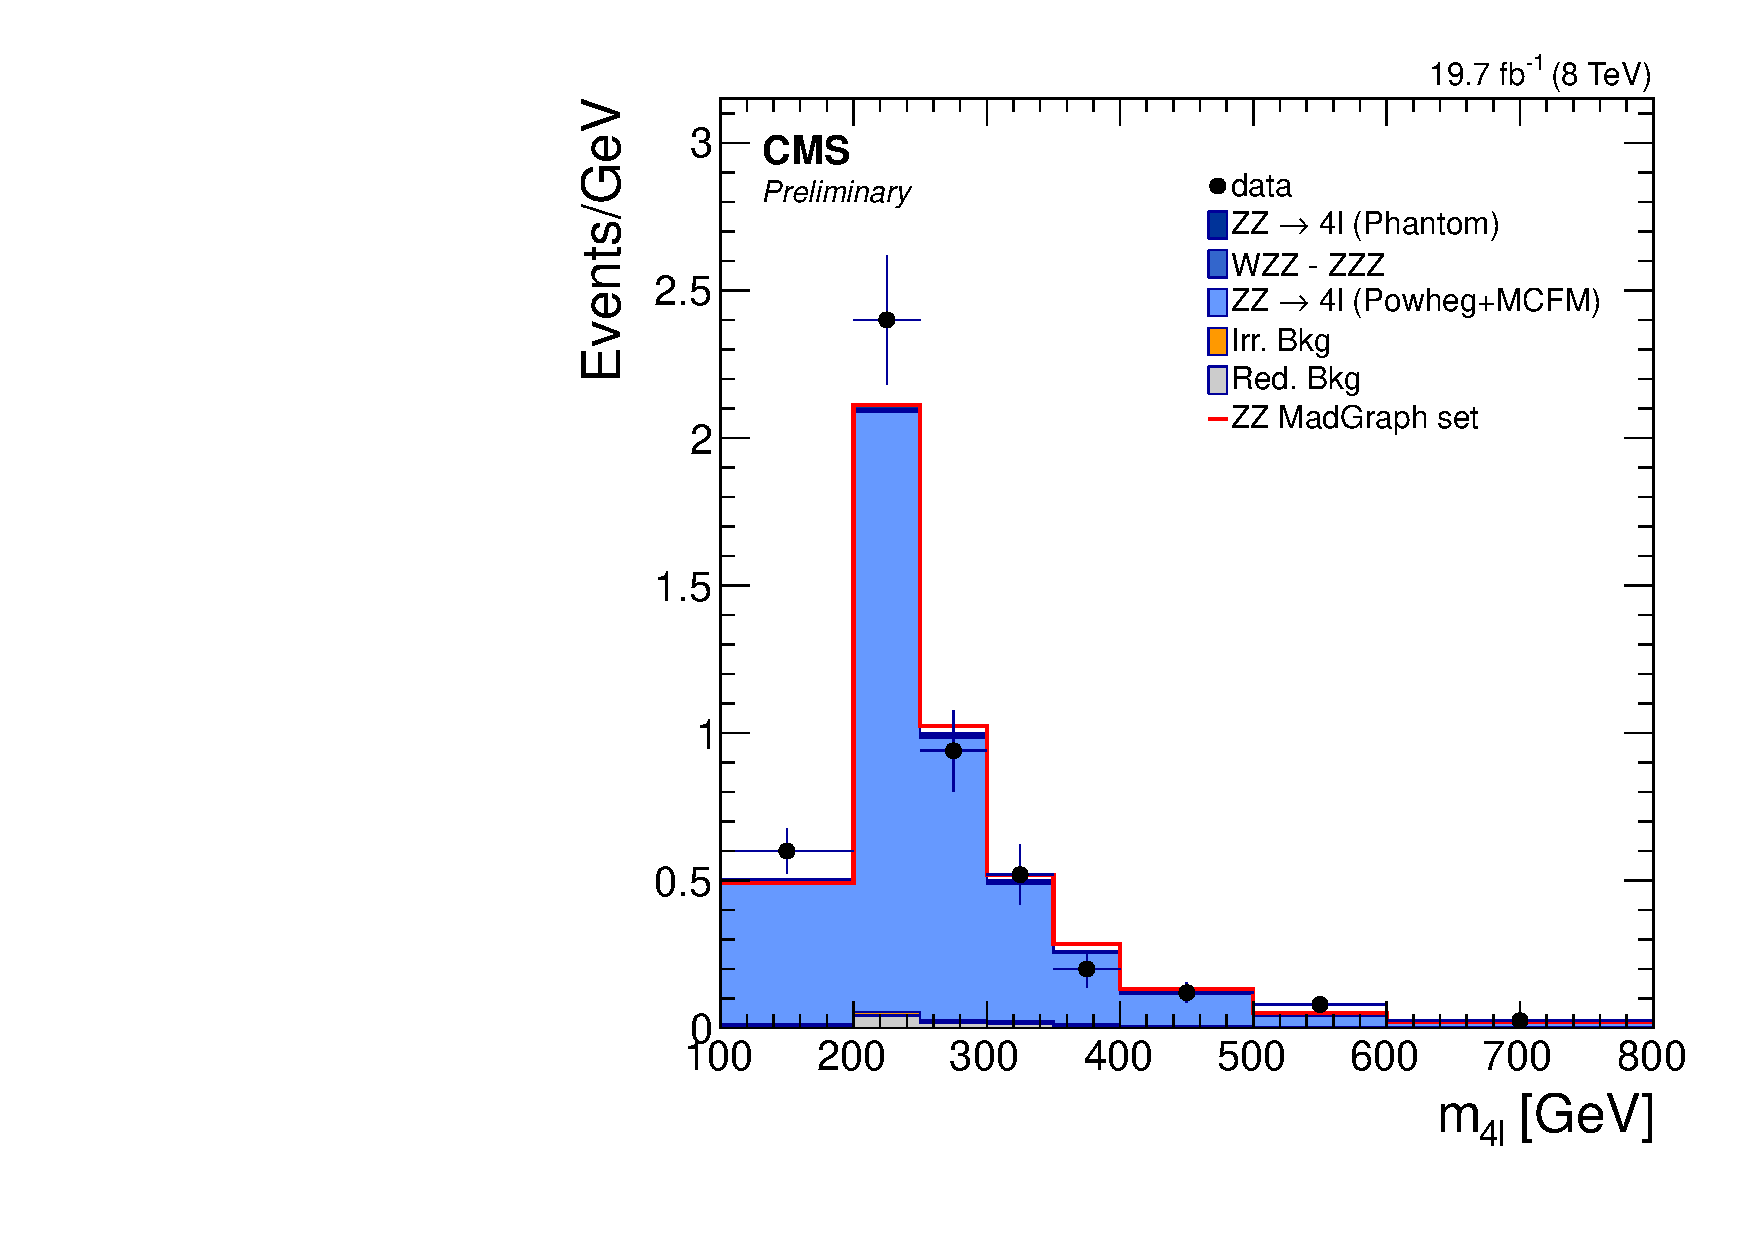
\includegraphics[width=\cmsFigWidth]{Figures/Mass_pow} 
    \caption{Different contributions to the distribution of the reconstructed four-lepton mass. Points represent the data, the stacked filled histogram represents the predictions for $ZZ$ signal and background contributions using \texttt{Powheg} samples to describe $q\bar{q}(qg)\to ZZ\to 4\ell$ processes (while for the stacked histogram outlined in red the \texttt{MadGraph} simulation is used).}
    \label{fig:sig_recoMass}
  \end{center}
\end{figure}
 
\begin{figure}[hbtp]
  \begin{center}
    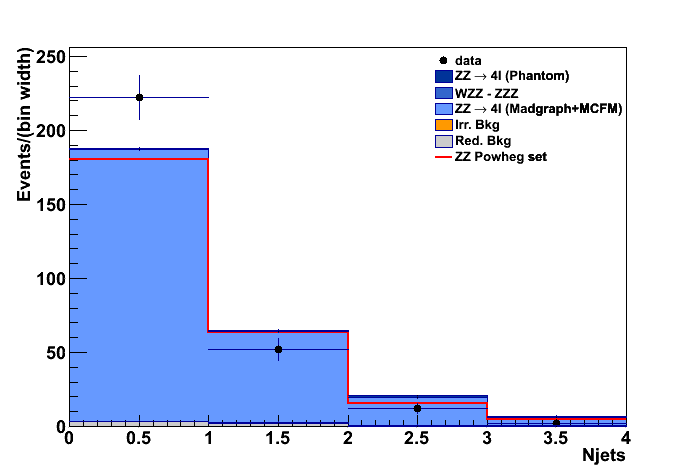
\includegraphics[width=\cmsFigWidth]{Figures/Jets_mad}
    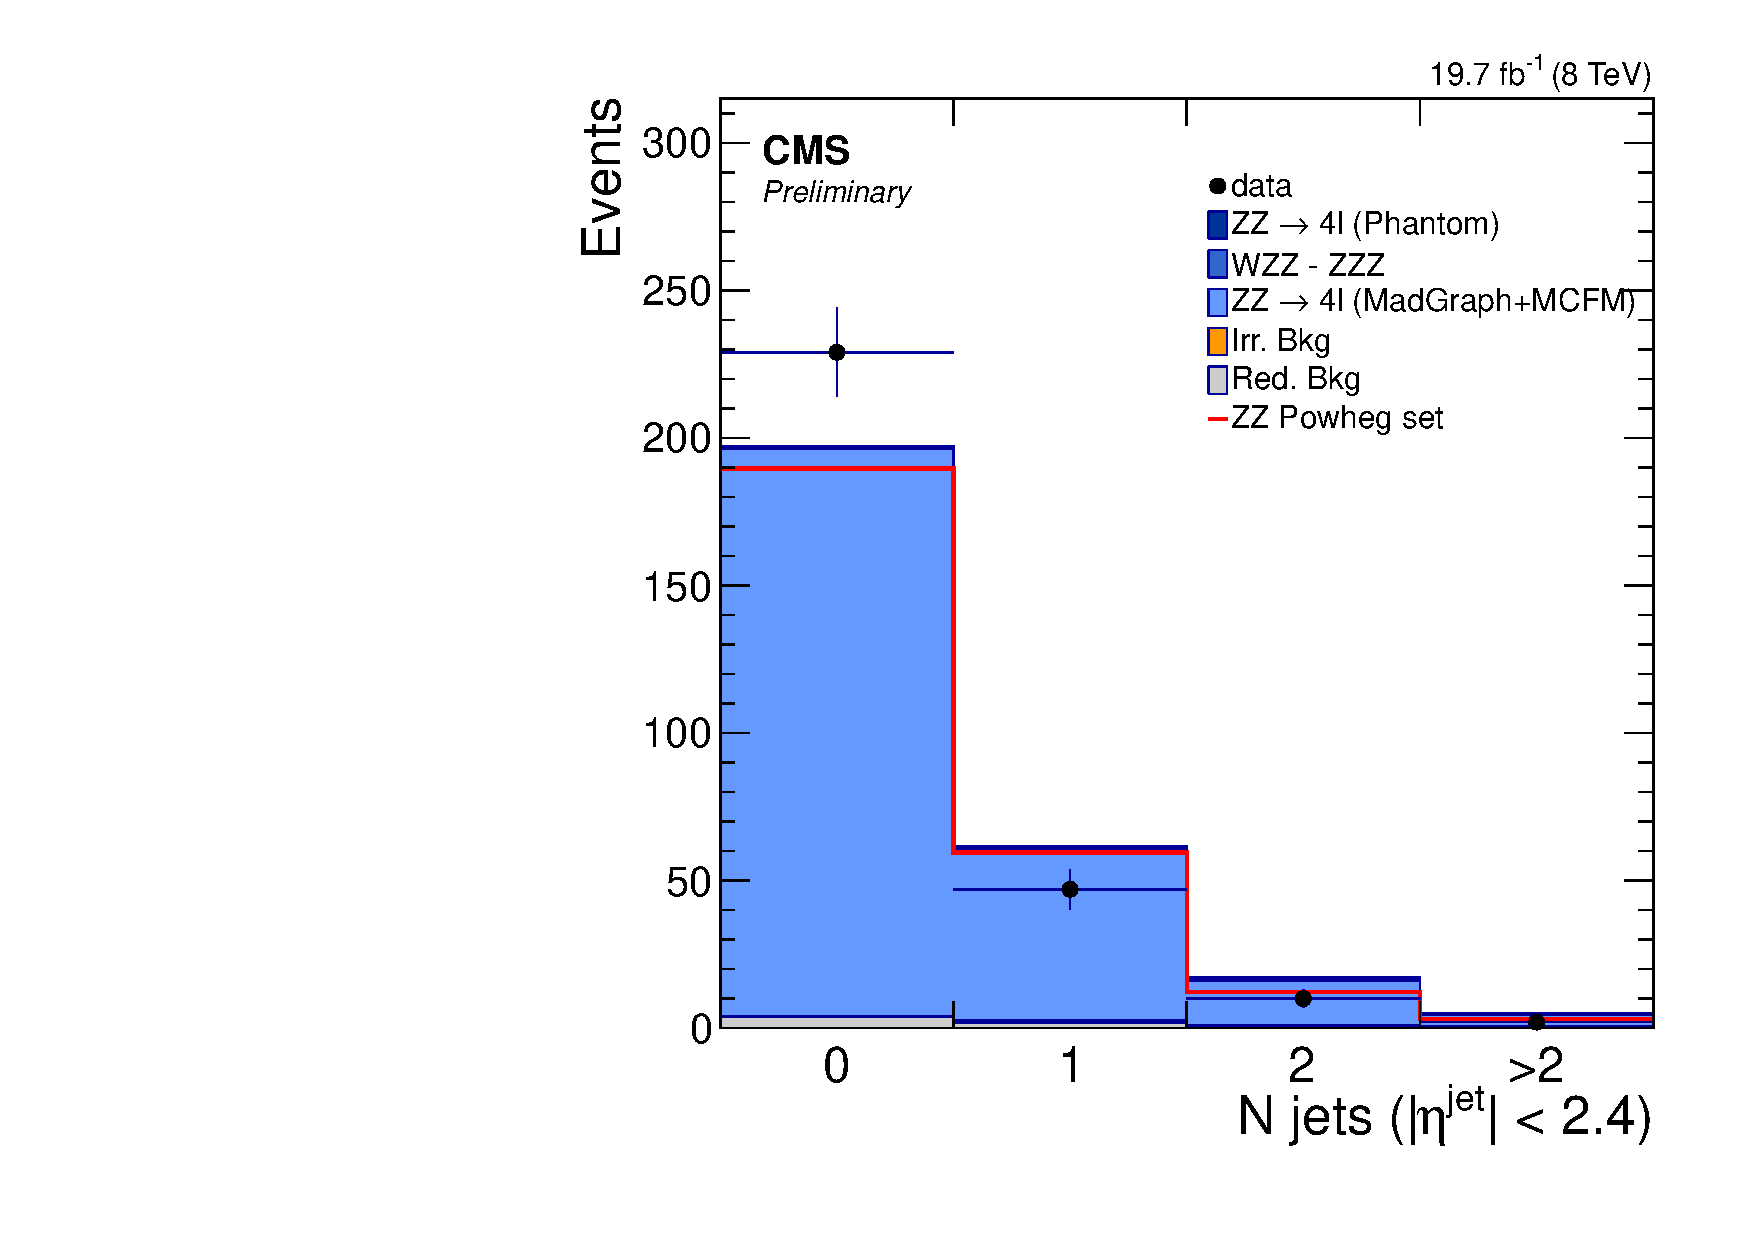
\includegraphics[width=\cmsFigWidth]{Figures/CentralJets_mad}
    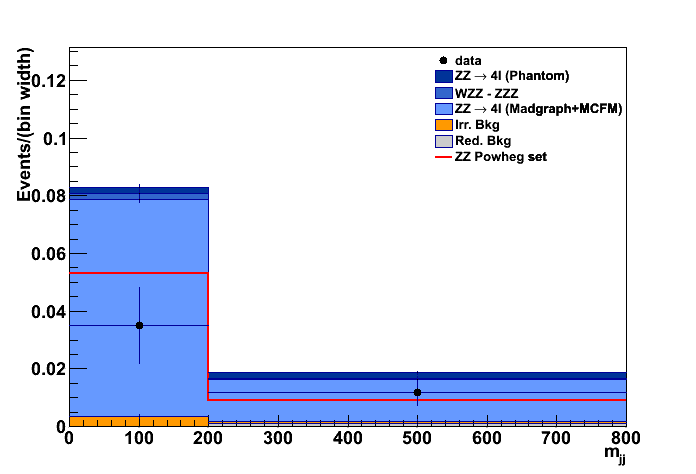
\includegraphics[width=\cmsFigWidth]{Figures/Mjj_mad}
    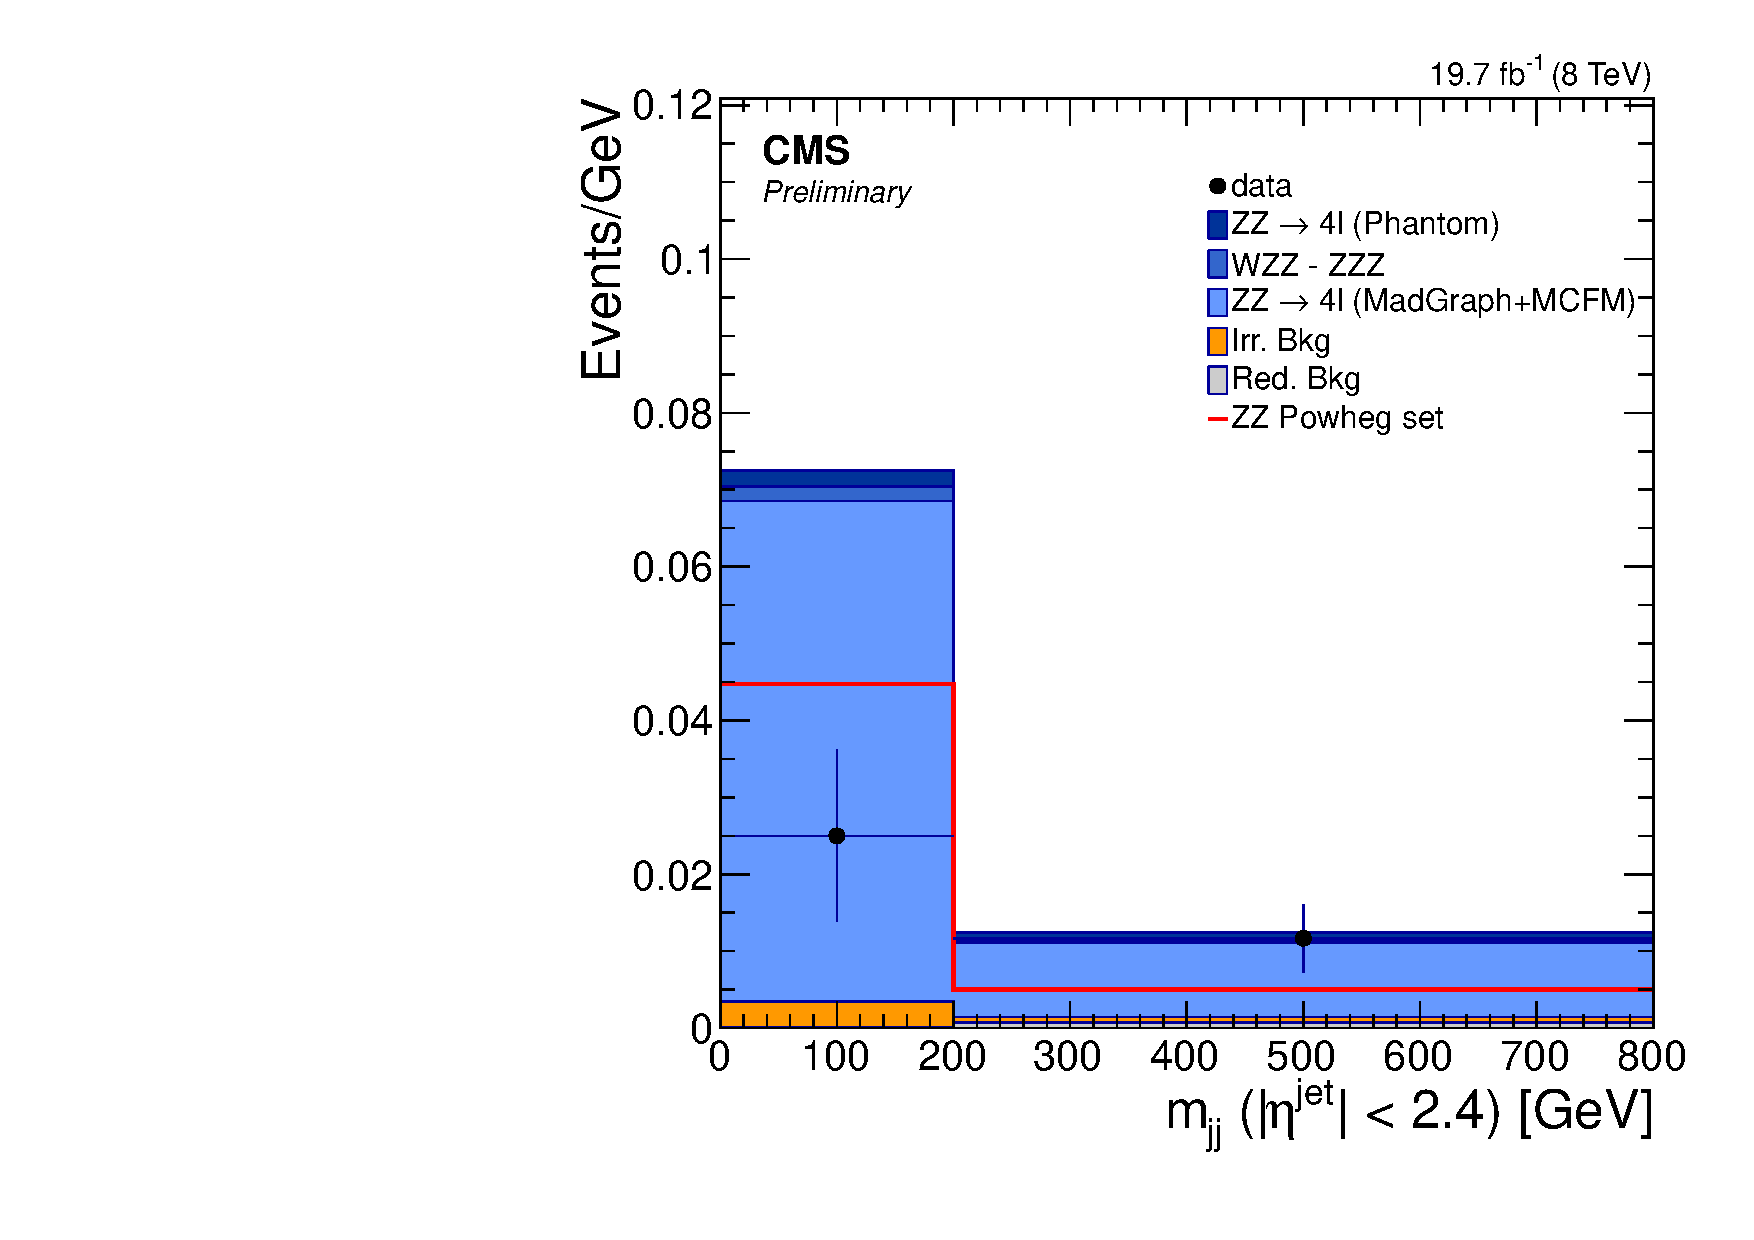
\includegraphics[width=\cmsFigWidth]{Figures/CentralMjj_mad} 
    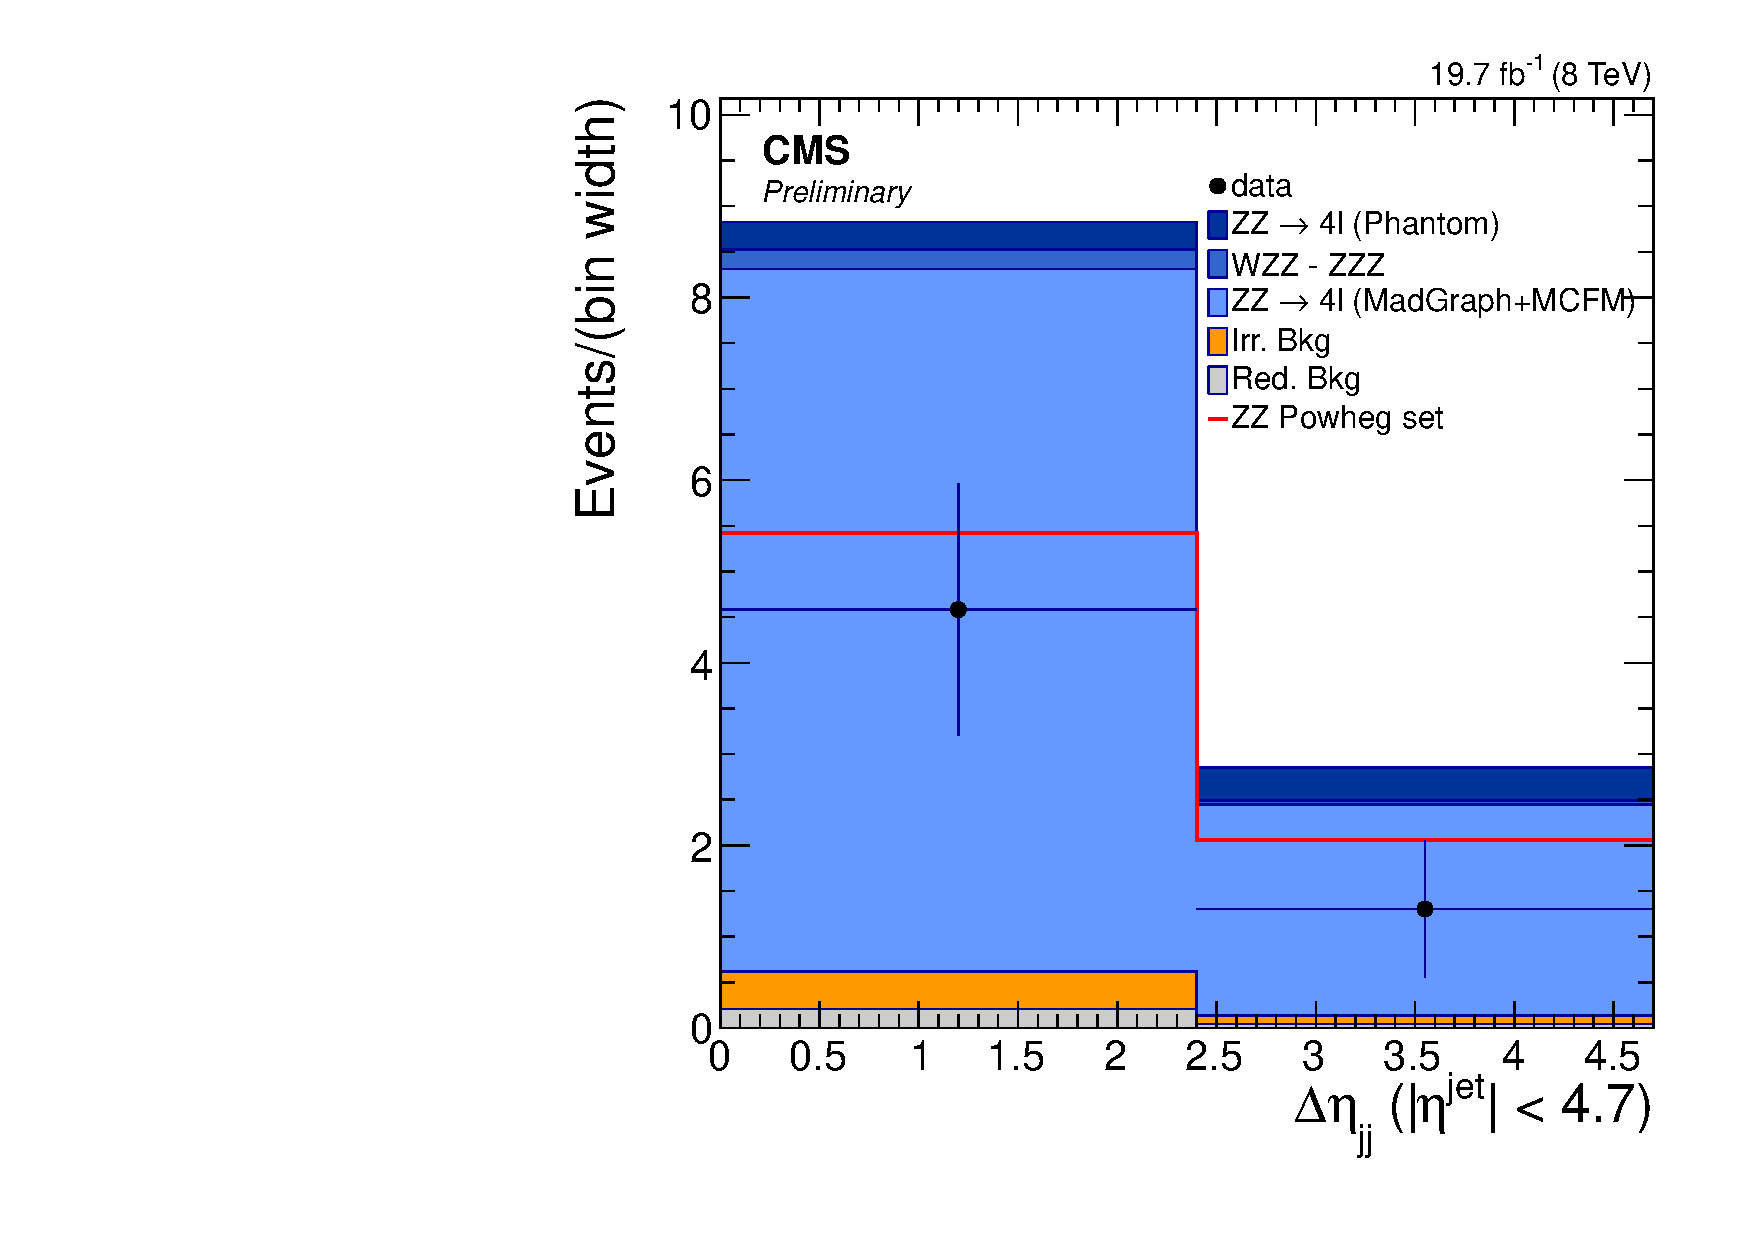
\includegraphics[width=\cmsFigWidth]{Figures/Deta_mad}  
    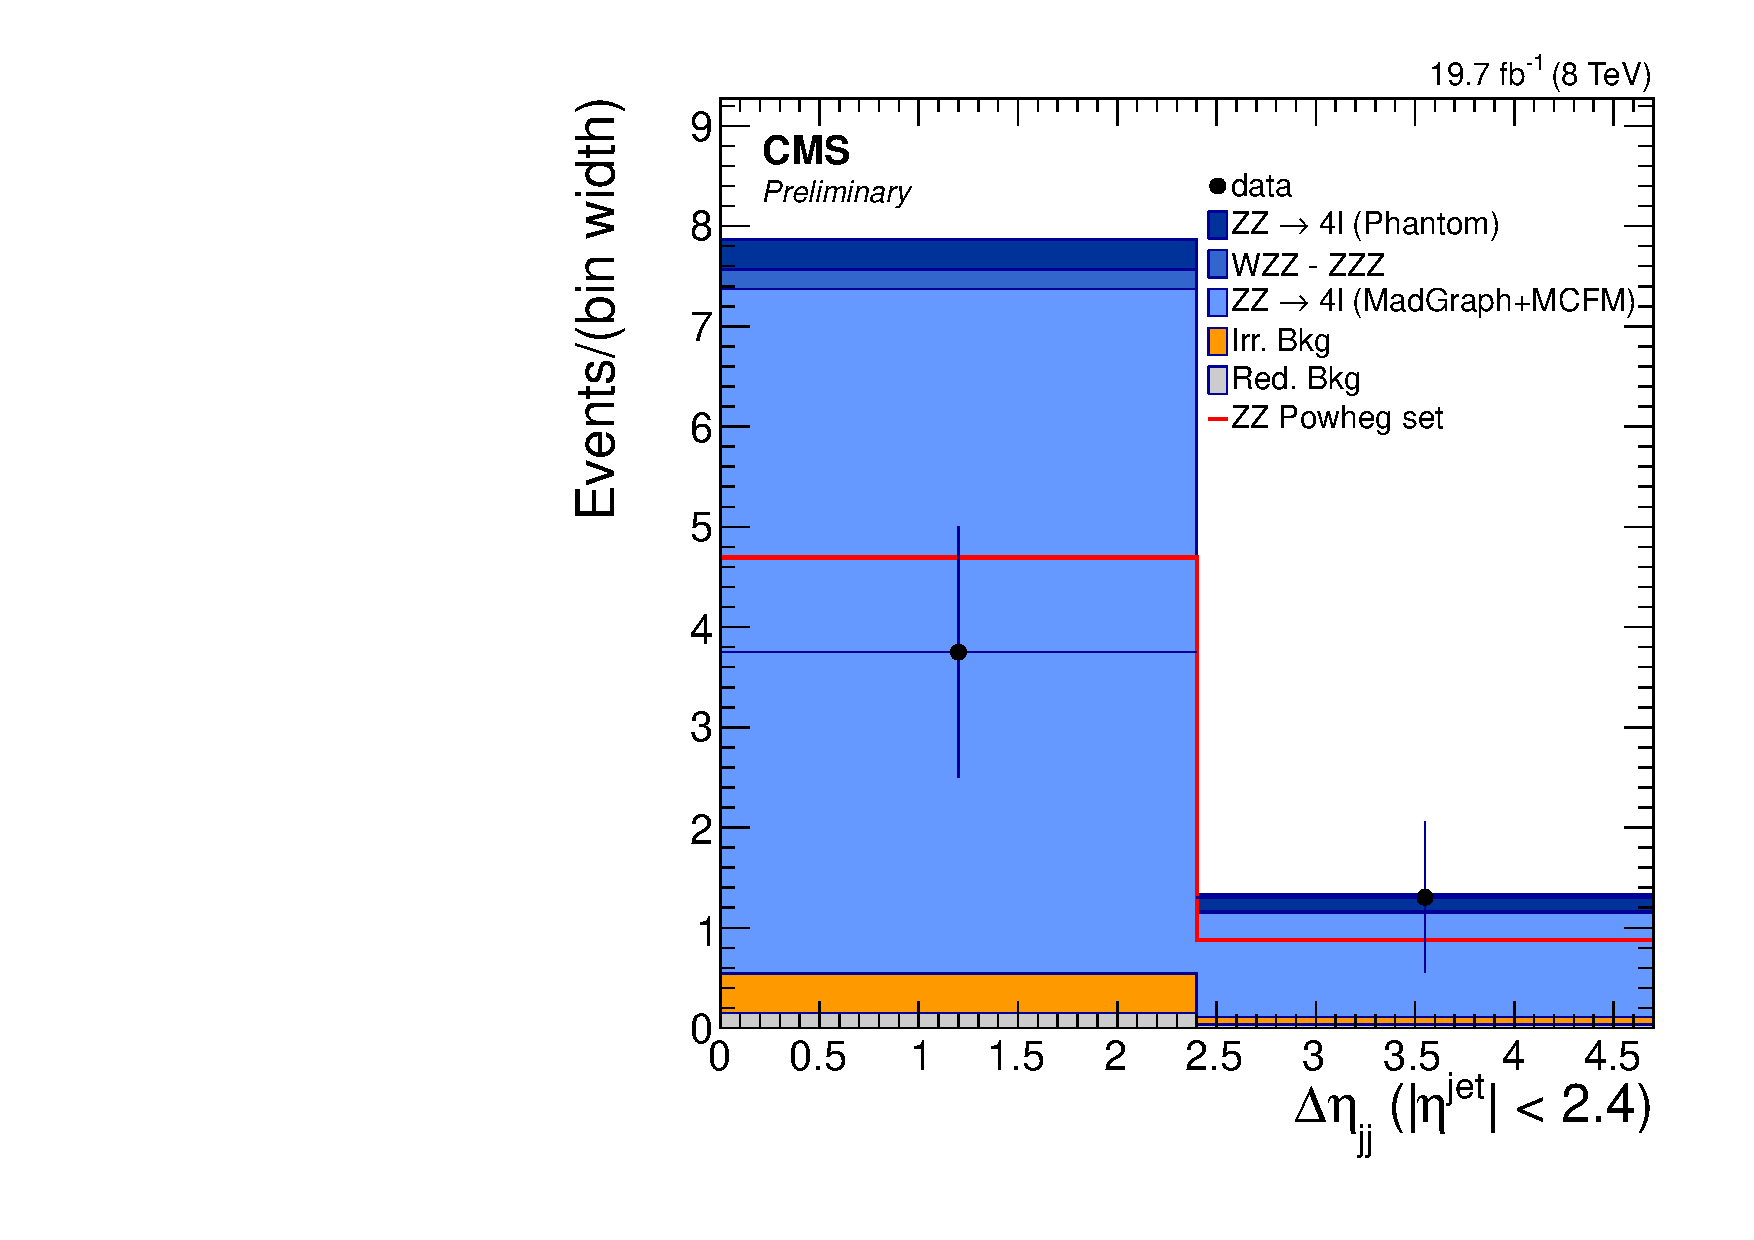
\includegraphics[width=\cmsFigWidth]{Figures/CentralDeta_mad}  
    \caption{Different contributions to the distribution of the reconstructed number of jets produced in the event (top), the invariant mass of the two most energetic jets (center) and the pseudorapidity interval between them (bottom), with $\eta^{jet} < 4.7$ on the left and $\eta^{jet} < 2.4$ on the right. Points represent the data, the stacked filled histogram represents the predictions for $ZZ$ signal and background contributions using \texttt{MadGraph} samples to describe $q\bar{q}(qg)\to ZZ\to 4\ell$ processes (while for the stacked histogram outlined in red the \texttt{Powheg} simulation is used).}
    \label{fig:sig_recoJJ}
  \end{center}
\end{figure}

\begin{figure}[hbtp]
  \begin{center} 
    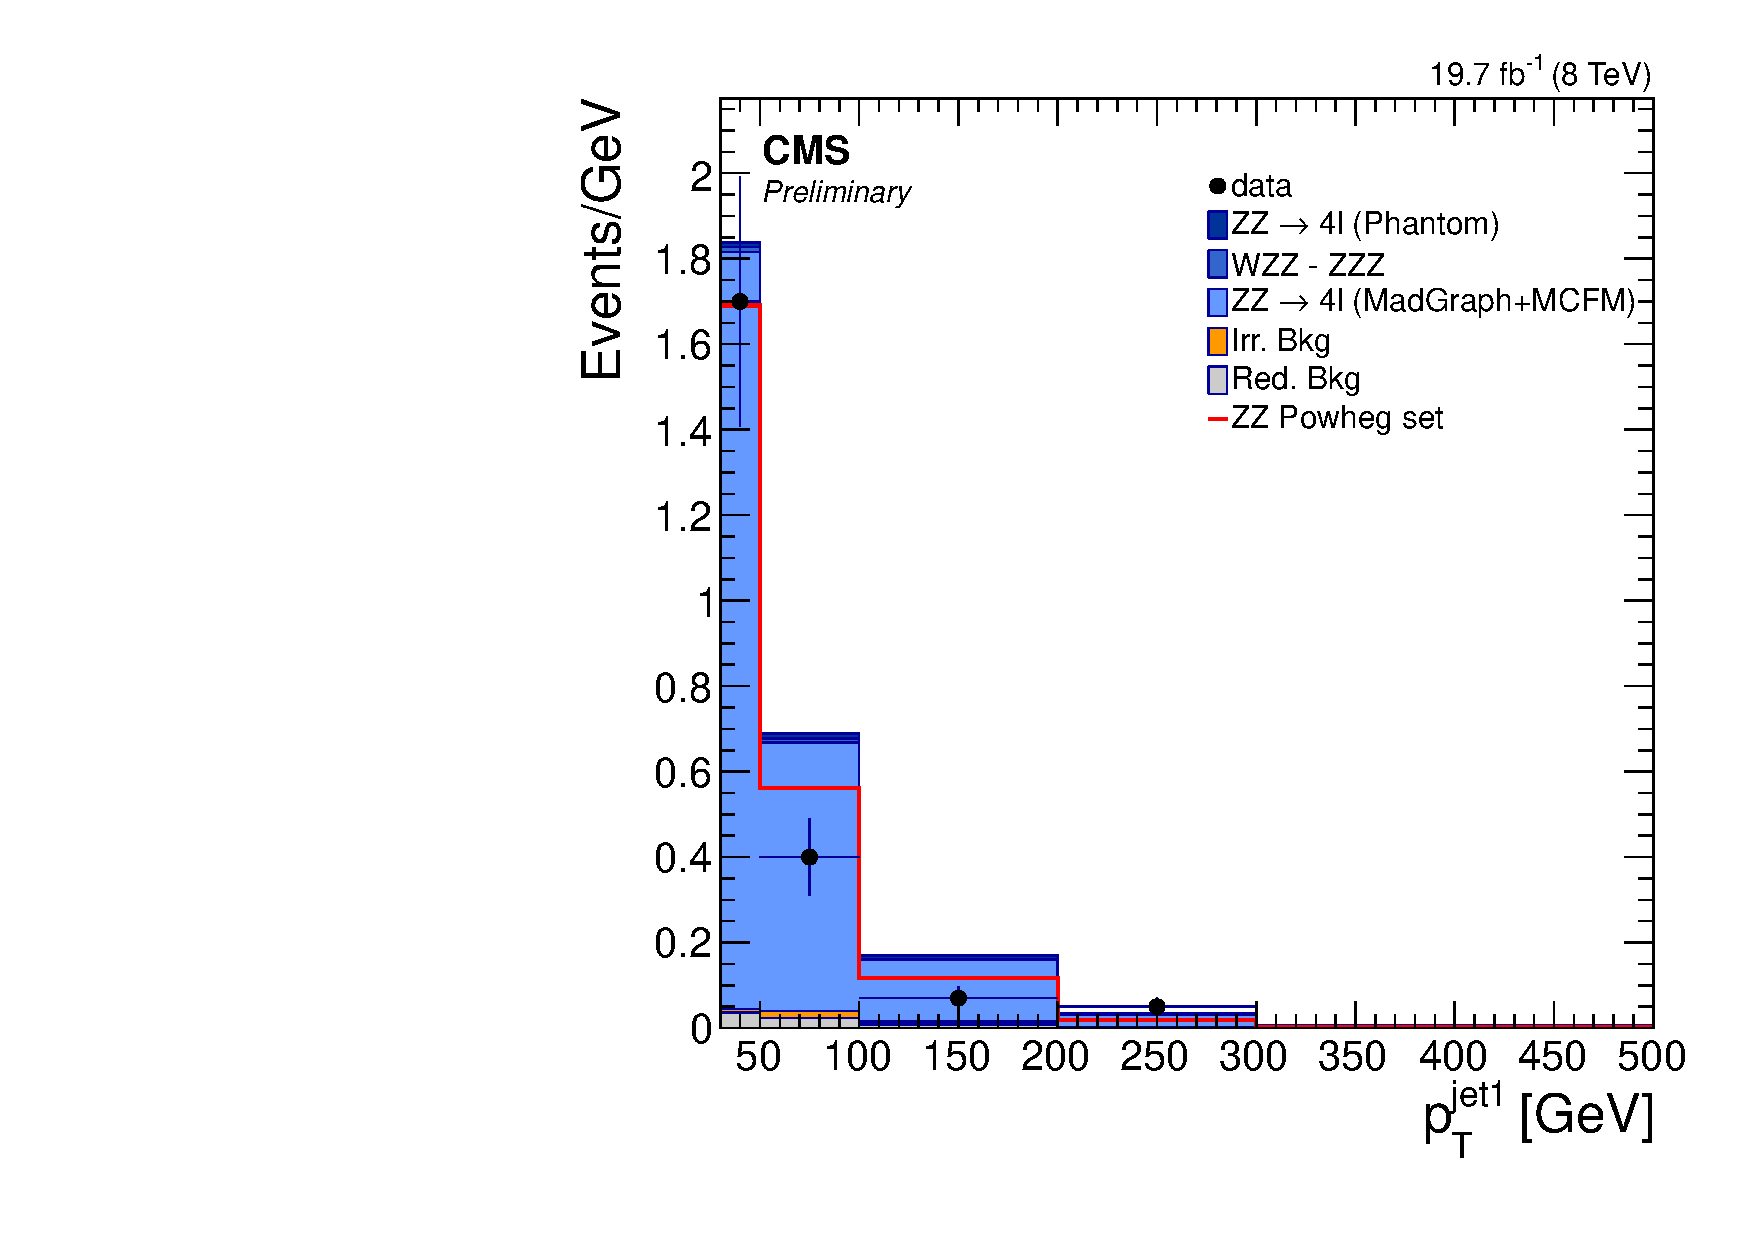
\includegraphics[width=\cmsFigWidth]{Figures/PtJet1_mad}
    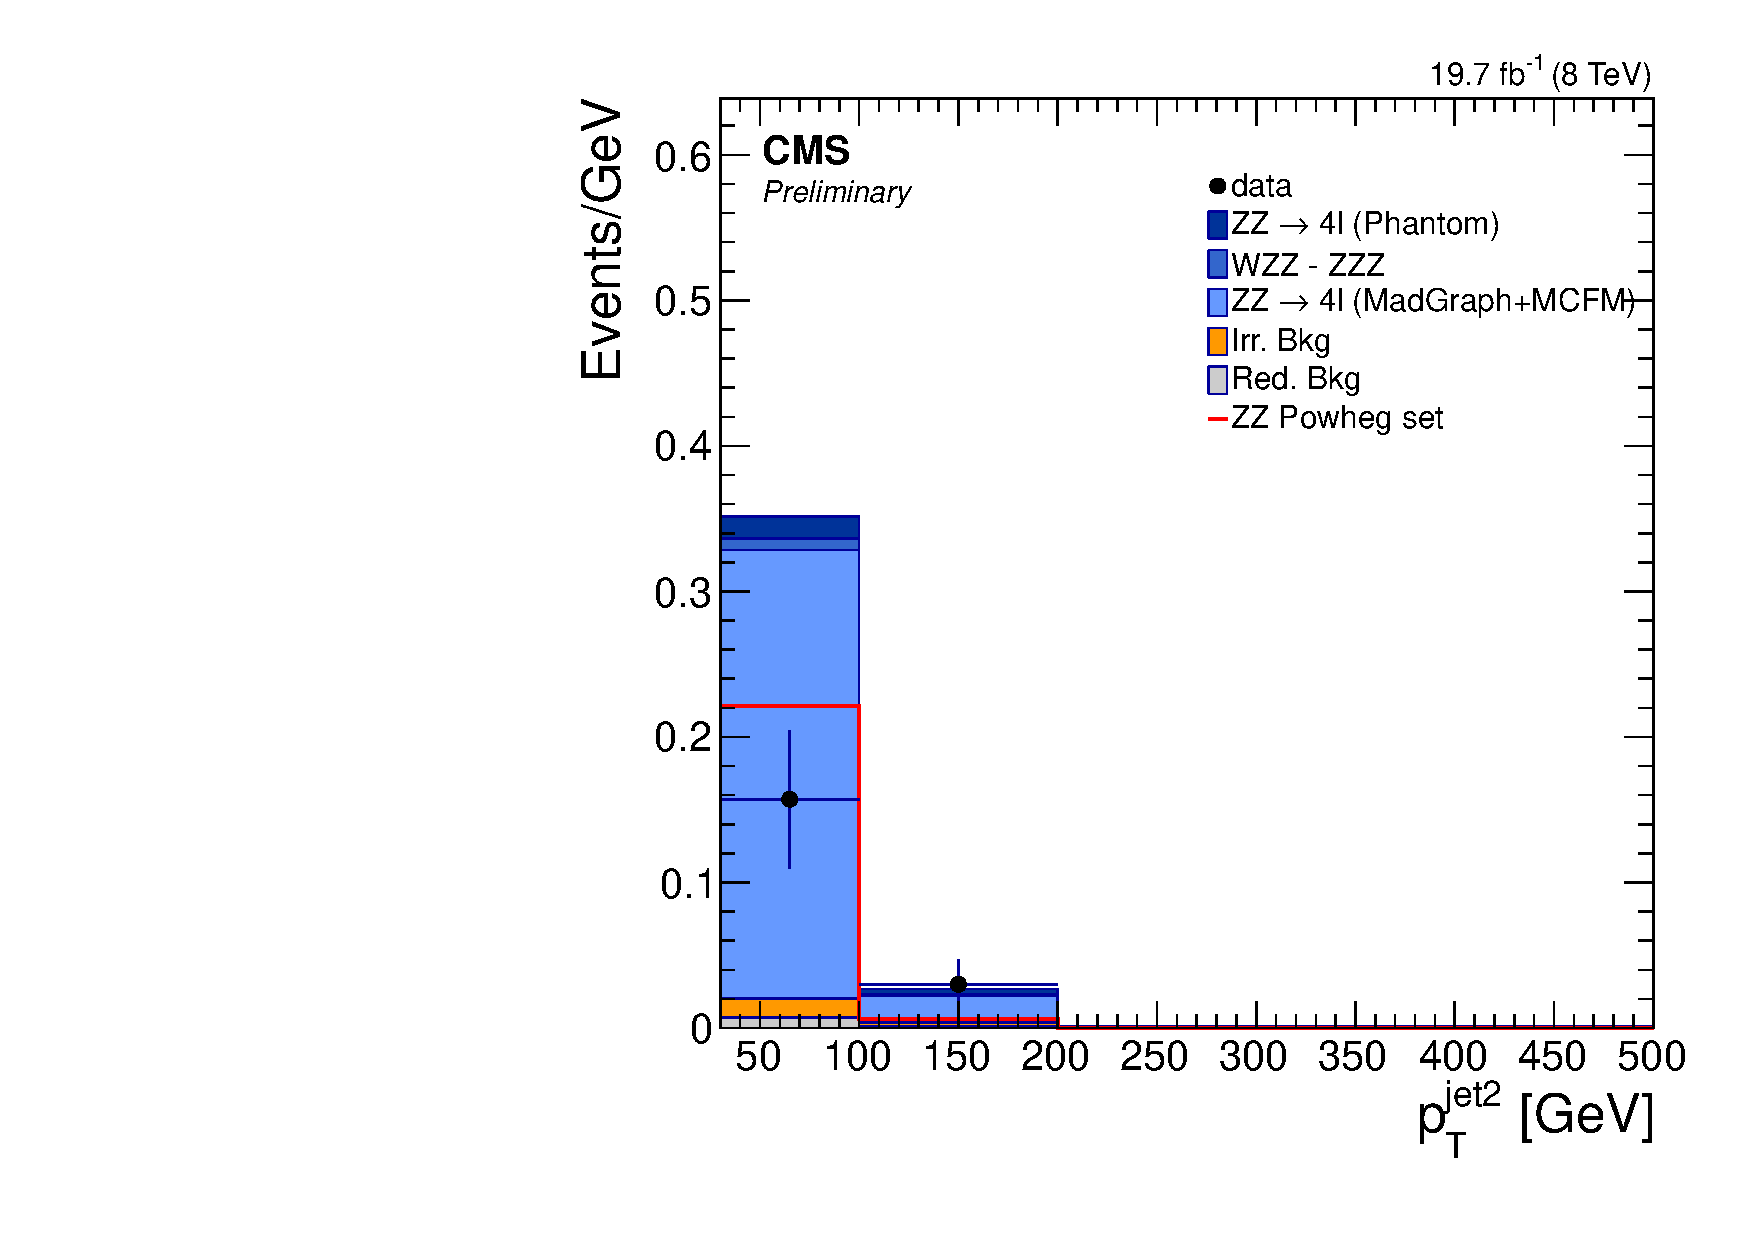
\includegraphics[width=\cmsFigWidth]{Figures/PtJet2_mad} 
    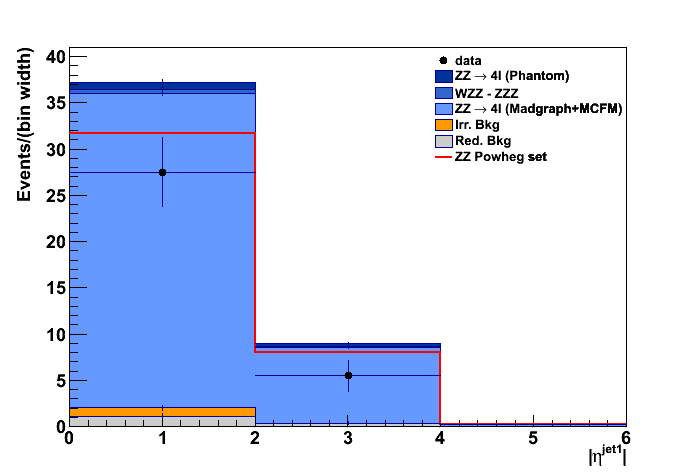
\includegraphics[width=\cmsFigWidth]{Figures/EtaJet1_mad}
    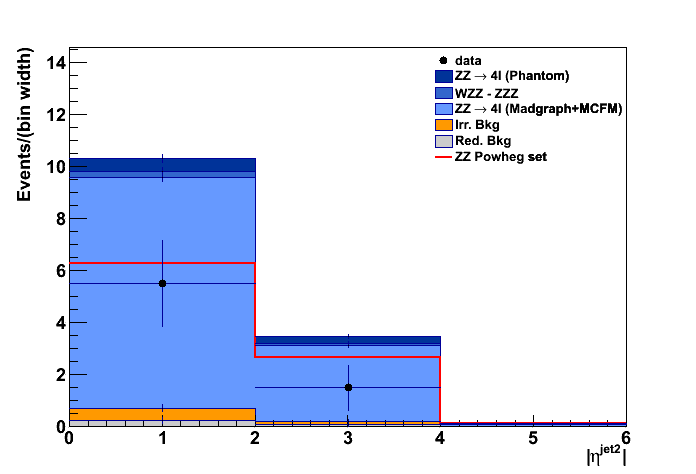
\includegraphics[width=\cmsFigWidth]{Figures/EtaJet2_mad}
    \caption{Different contributions to the distribution of the reconstructed transverse momentum (top) and pseudorapidity (bottom) of the leading (left) and  sub-leading jet (right). Points represent the data, the stacked filled histogram represents the predictions for $ZZ$ signal and background contributions using \texttt{MadGraph} samples to describe $q\bar{q}(qg)\to ZZ\to 4\ell$ processes (while for the stacked histogram outlined in red the \texttt{Powheg} simulation is used).}
    \label{fig:sig_recoPt}
  \end{center}
\end{figure}


\begin{figure}[hbtp]
  \begin{center}
   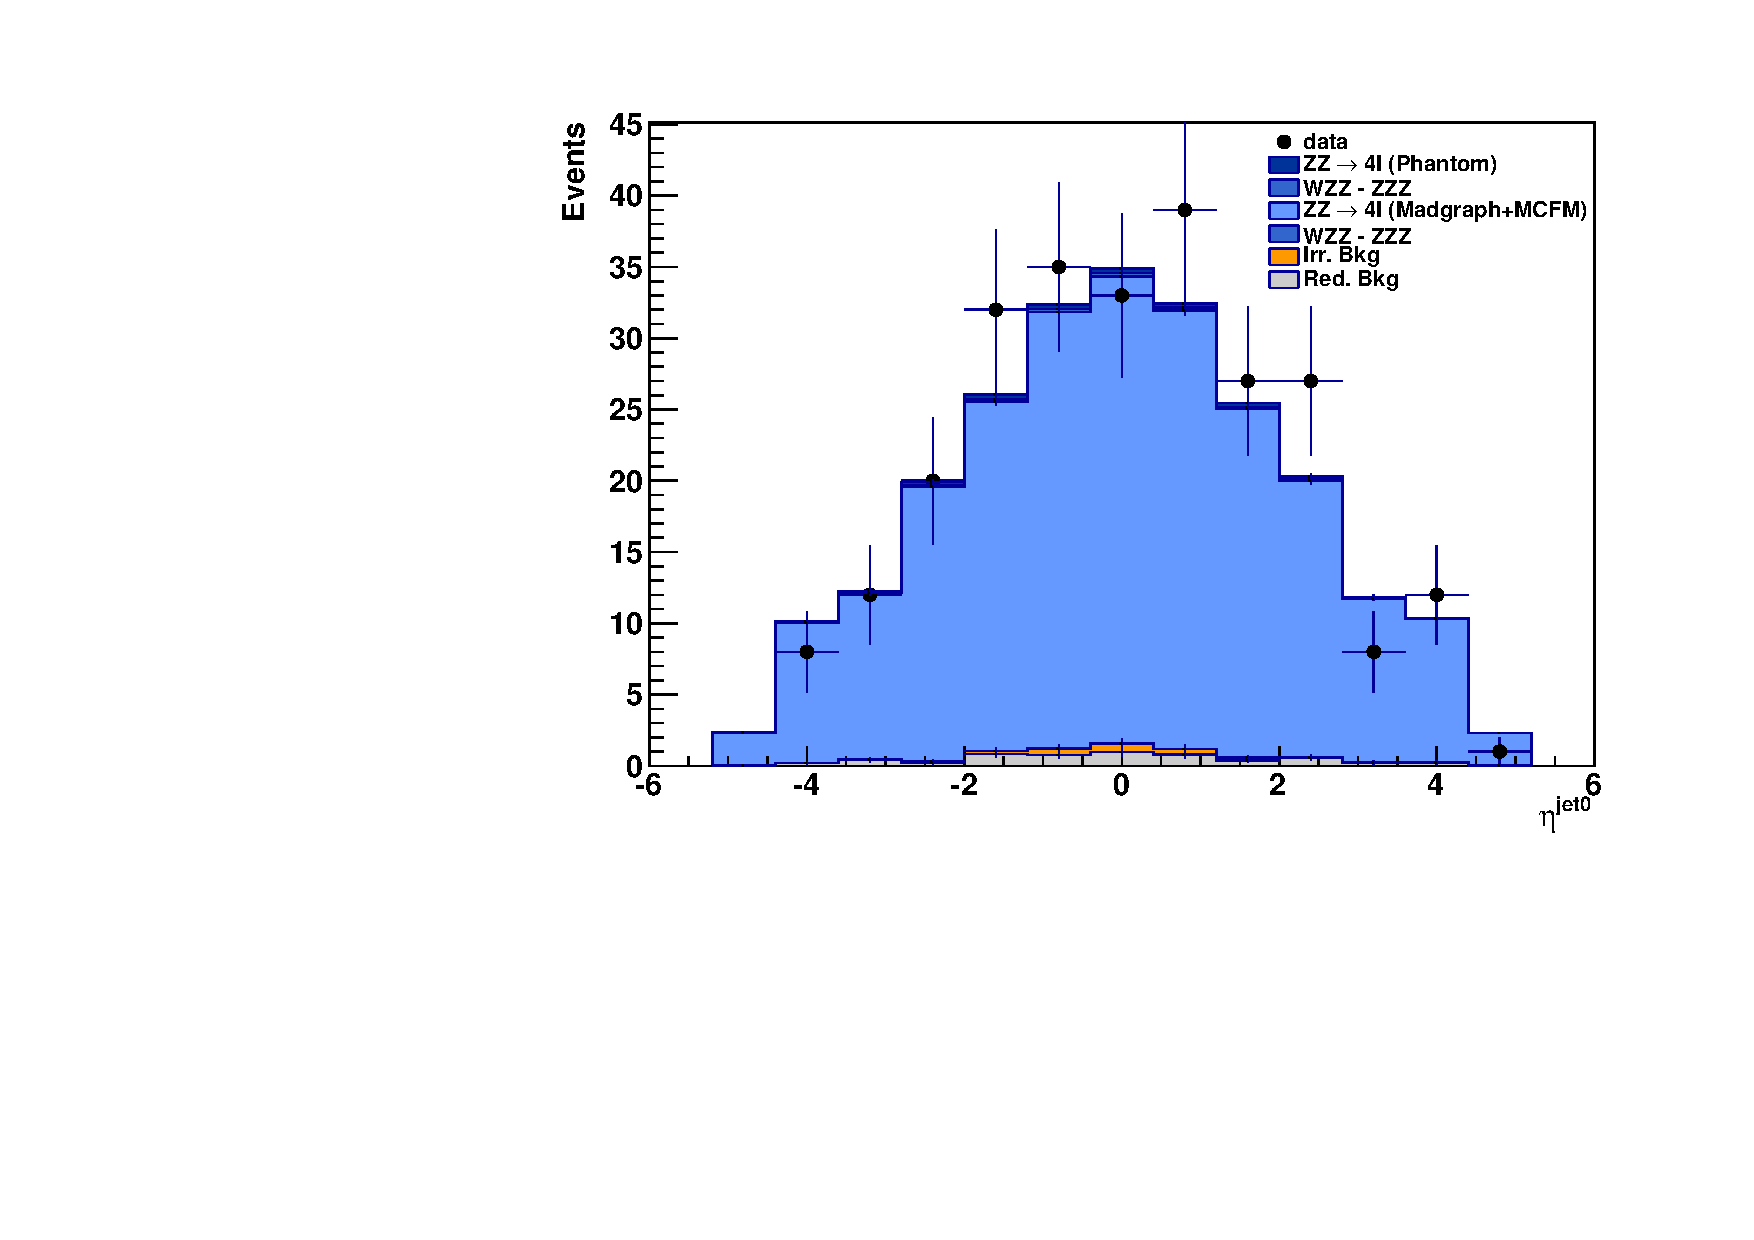
\includegraphics[width=0.8\cmsFigWidth]{Figures/Eta0_mad}    
   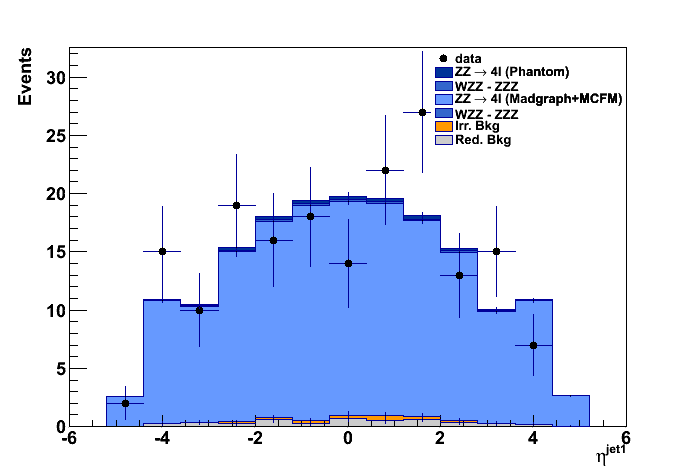
\includegraphics[width=0.8\cmsFigWidth]{Figures/Eta1_mad}
   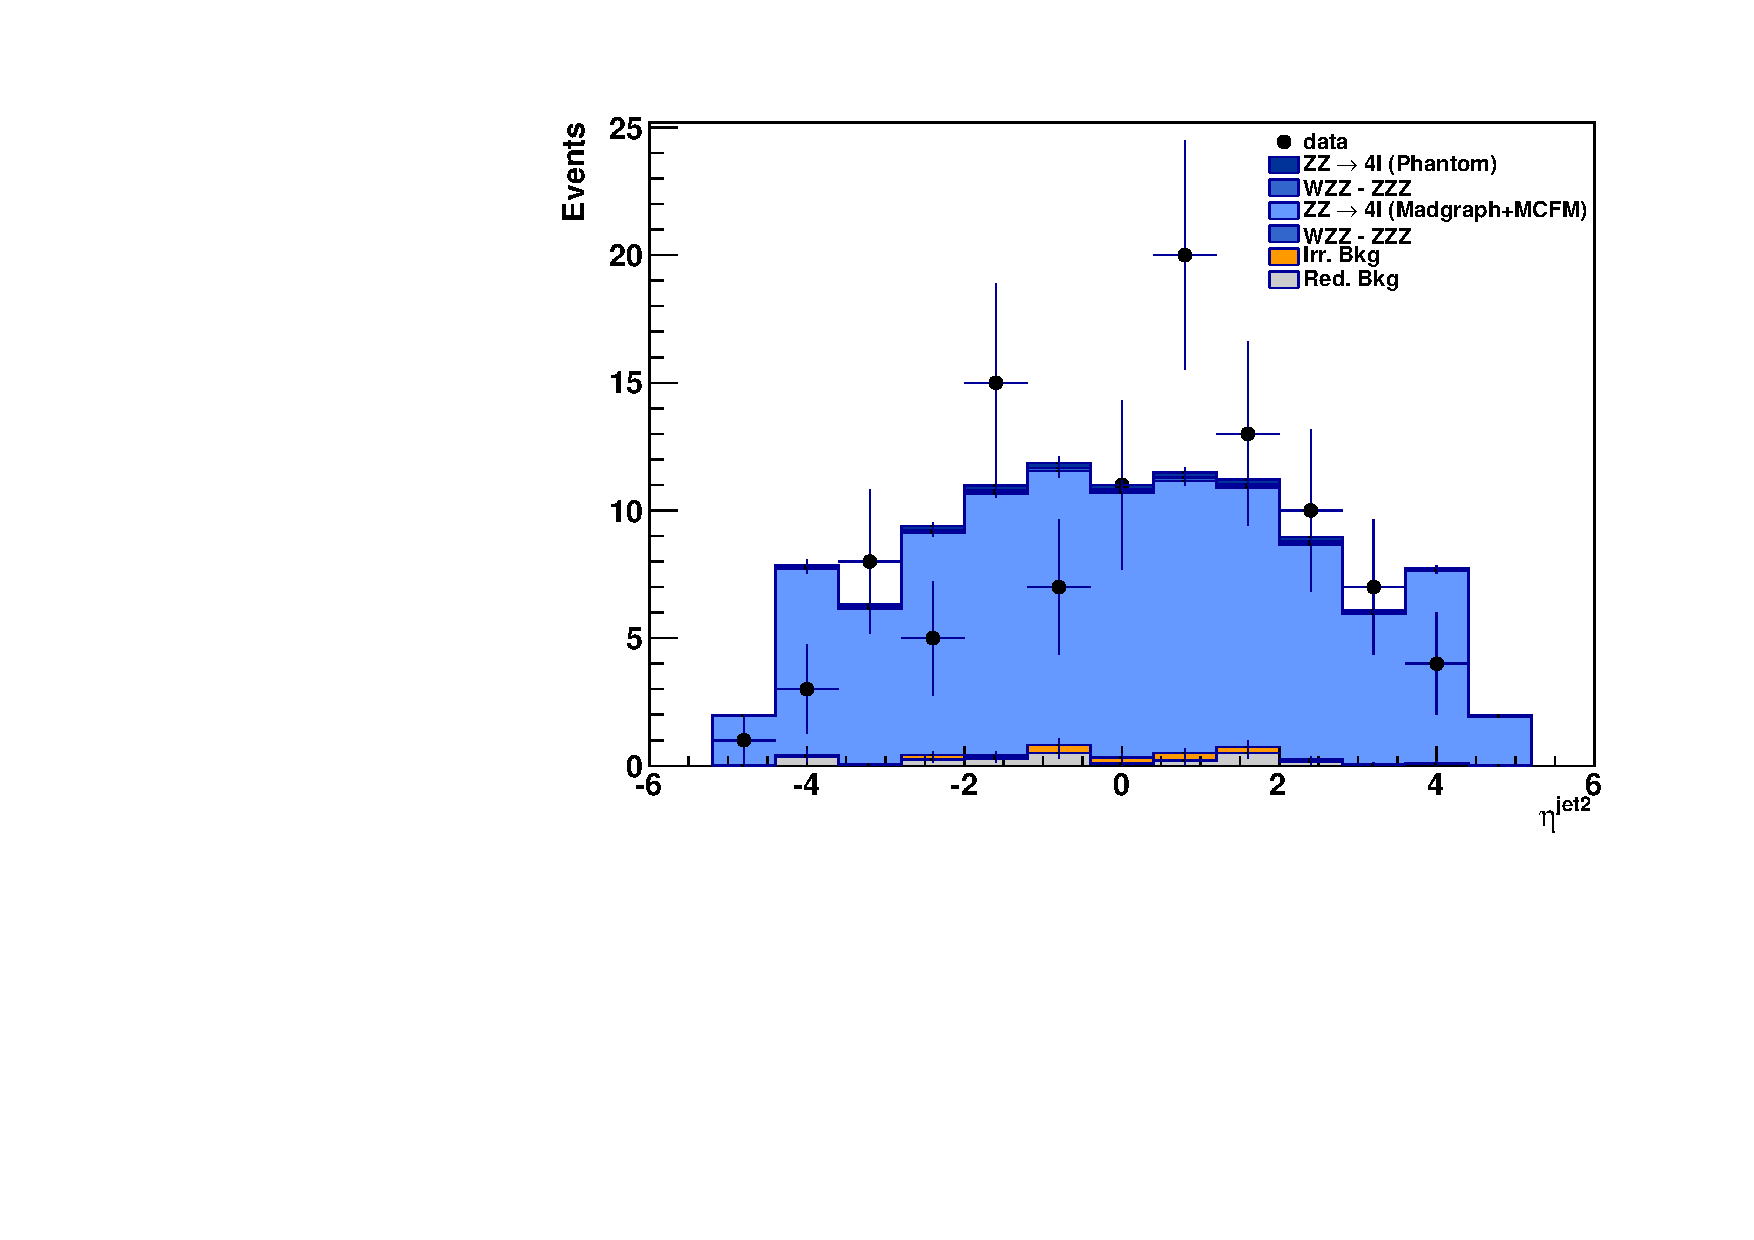
\includegraphics[width=0.8\cmsFigWidth]{Figures/Eta2_mad}
   \caption{Different contributions to the $\eta$-distribution of the most energetic (\cmsLeft), second most energetic (center) and third most energetic (\cmsRight) jet in the event, considering $p_T^{jet}> 10~\mathrm{GeV}$}
   \label{fig:eta_jets}
  \end{center}
\end{figure}
\begin{figure}[hbtp]
  \begin{center}
   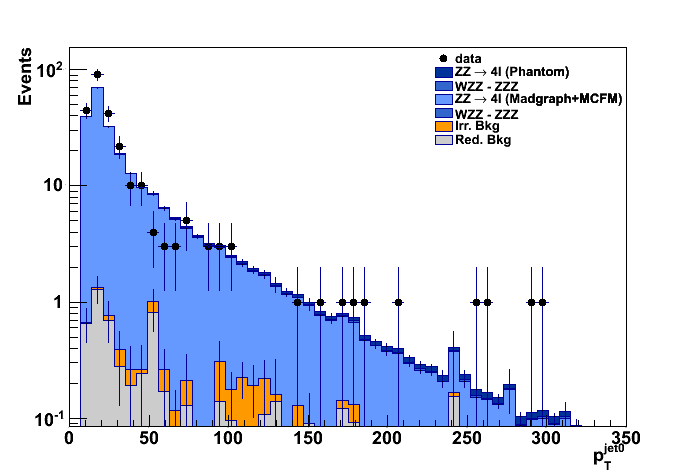
\includegraphics[width=0.8\cmsFigWidth]{Figures/Pt0_mad_log}    
   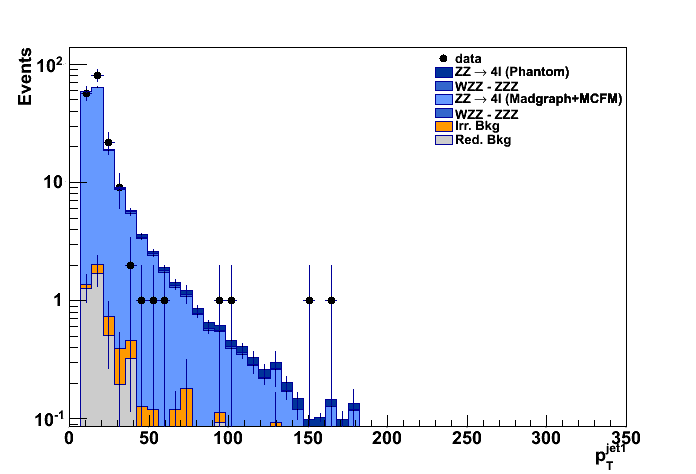
\includegraphics[width=0.8\cmsFigWidth]{Figures/Pt1_mad_log}
   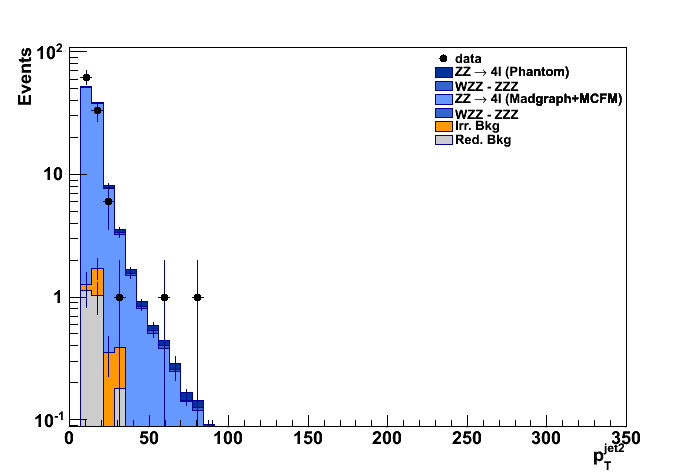
\includegraphics[width=0.8\cmsFigWidth]{Figures/Pt2_mad_log}
   \caption{Different contributions to the $p_{T}$-distribution of the most energetic (\cmsLeft), second most energetic (center) and third most energetic (\cmsRight) jet in the event, considering  $p_T^{jet}> 10~\mathrm{GeV}$.}
   \label{fig:pt_jets}
  \end{center}
\end{figure}
Table~\ref{tab:xs} lists the total cross-section obtained from each individual decay channel as well as the
total cross-section based on the combination of all channels. The measured cross-section agrees
with the theoretical value of $7.5\pm 0.5$ pb calculated with \texttt{MCFM 6.6}. In this calculation, the
contribution from $q\bar{q} \to ZZ$ is obtained at NLO, while the smaller contribution (approximately
6\%) from $ gg \to ZZ$ is obtained at LO.

\begin{table*}[htbH]
\begin{center}
\topcaption{The signal yield is obtained by subtracting from the observed yield the expected background events. Statistical uncertainties are reported.
\label{tab:sig_yields}}
\begin{tabular}{lcccc}
\hline Final state & Observed data& Irreducible background & Reducible background & Final yield\\
\hline $ZZ\to 4\mu $ & $ 80 \pm 8.9 $ & $ 0.52 \pm 0.10 $ & $ 0.92 \pm 0.61 $ & $ 78.6 \pm 8.9$ \\ 
$ZZ\to 4e $ & $56 \pm 7.5 $ & $ 0.21 \pm 0.06 $ & $ 1.93 \pm 0.72 $ & $ 54.0 \pm 7.5 $\\
$ZZ\to 2e2\mu$ & $ 152 \pm 12 $ & $ 1.16 \pm 0.15 $ & $ 3.3 \pm 1.1 $ & $ 148 \pm 12 $\\
\hline
\textbf{$ZZ\to 4\ell$} & $ 288 \pm 17 $ & $1.89 \pm 0.19 $ & $ 6.2 \pm 1.4 $ & $ 281 \pm17 $ \\ 
\hline 
\end{tabular}
\end{center}
\end{table*}

%\begin{table*}[htbH]
%\begin{center}
%\topcaption{The total $ZZ$ production cross-section as measured in each decay channel and for the
%combination of all channels.
%\label{tab:xs}}
%\begin{tabular}{lc}
%\hline Final state & Total cross-section [pb]\\
%\hline $ZZ\to 4\mu $ & $7.5\pm 0.9$ (stat.) $\pm 0.3$ (syst.)\\
%$ZZ\to 4e $ &  $7.4\pm 1.0$ (stat.) $\pm 0.3$ (syst.)\\
%$ZZ\to 2e2\mu$ & $8.3\pm 0.7$ (stat.) $\pm 0.4$ (syst.)\\
%\hline
%\textbf{$ZZ\to 4\ell$} &  $7.6\pm 0.5$ (stat.) $\pm 0.3$ (syst.)\\
%\hline \\
%\end{tabular}
%\end{center}
%\end{table*}
\begin{table*}[htbH]
\begin{center}
\caption{The total $ZZ$ production cross-section as measured in each decay channel and for the
combination of all channels in the fiducial region $60< m_{Z_{1}}, m_{Z_{}} < 120~\mathrm{GeV}$.}
\label{tab:xs}
%\scalebox{1.5\columnwidth}{!}{
%\doublespacing{
\begin{tabular}{lc}
\hline Process & Total cross-section [pb]\\
\hline $pp\to ZZ(4\mu) $ & $7.46\pm 0.86~\mathrm{(stat.)}^{+0.45}_{- 0.47}~\mathrm{(syst.)}$\\
$pp\to ZZ(4e) $ &  $7.32\pm 1.02~\mathrm{(stat.)}^{+0.59}_{- 0.62}~\mathrm{(syst.)}$\\
$pp\to ZZ(2e2\mu)$ & $8.22\pm 0.70~\mathrm{(stat.)}^{+0.59}_{- 0.61}~\mathrm{(syst.)}$\\
\hline
\textbf{$pp\to ZZ(4\ell)$} & $7.76 \pm 0.48~\mathrm{(stat.)}^{+0.47}_{- 0.47}~\mathrm{(syst.)}$ \\
\hline \\
\end{tabular}%}
\end{center}
\end{table*}
The fiducial region in which the cross-section is extracted, defined requiring two $Z$ bosons with mass between 60 and 120 GeV, is much wider with respect to the region in which events are really measured, limited by the active volume of the detector, as shown by the low values of $A\cdot \epsilon$. In order to obtain a measurement closer to what is effectively reconstructed by the detector, a \emph{tight fiducial region} is defined as follows:
\begin{itemize}
\item $60 < m_{Z_1},m_{Z_2} < 120~\mathrm{GeV}$;
%\item $m_{4\ell} > 100~\mathrm{GeV}$;
\item at least one lepton with $p_T > 20~\mathrm{GeV}$ and another one with $p_T > 10~\mathrm{GeV}$;
\item electrons must have $p_T^e > 7~\mathrm{GeV}$ and $|\eta^e|<2.5$;
\item muons must have $p_T^{\mu} > 5~\mathrm{GeV}$ and $|\eta^{\mu}|<2.4.$
\end{itemize}
The last three requirements correspond to the $\eta$ and $p_T$-acceptance of the detector and are the same selection criteria demanded when leptons are built, while the first requirement corresponds to the definition of the wider region applied for the previous inclusive measurement. The formula used in this case is
$$\sigma_{ZZ} = \frac{N_{data}-N_{bkg}}{\mathcal{L}\cdot A \cdot \epsilon},$$
where the branching-ratio factor is removed in order to obtain the cross-section of the $pp\to ZZ\to 4\ell$ process, and the new values of $ A \cdot \epsilon$ are reported in Table~\ref{tab:Aeps_tight}. The cross-section measurements obtained in this tight region are listed in Table~\ref{tab:tightxs}.
\begin{table*}[htbH]
\begin{center}
\topcaption{$A\cdot \epsilon$ for the three final states used in the $pp\to ZZ \to 4\ell$ cross-section measurement in the tight fiducial region.
The values reported are a product of the detector geometrical acceptance and
the object reconstruction and event identification efficiency. \label{tab:Aeps_tight}}
\begin{tabular}{cc}
\hline Final State & $A\cdot\epsilon$\\
\hline $4\mu$ & 84 \%  \\
$4e$ & 55\%\\
$2e2\mu$ & 69\%\\
\hline
\end{tabular}
\end{center}
\end{table*}
\begin{table*}[htbH]
\begin{center}
\topcaption{The total $ZZ$ production cross-section as measured in each decay channel and for the
combination of all channels in the tight fiducial region.
\label{tab:tightxs}}
\begin{tabular}{lc}
\hline Final state & Total cross-section [fb]\\
\hline $ZZ\to 4\mu $ & $4.74\pm 0.54$ (stat.) $^{+0.17}_{-0.18}$ (syst.)\\
$ZZ\to 4e $ &  $4.99\pm 0.69$ (stat.) $^{+0.32}_{-0.35}$ (syst.)\\
$ZZ\to 2e2\mu$ & $10.77\pm 0.90$ (stat.) $^{+0.55}_{-0.59}$ (syst.)\\
\hline
\textbf{$ZZ\to 4\ell$} &  $20.50\pm 1.26$ (stat.) $^{+0.82}_{-0.85}$ (syst.)\\
\hline \\
\end{tabular}
\end{center}
\end{table*}

\begin{figure}[hbtp]
  \begin{center}
    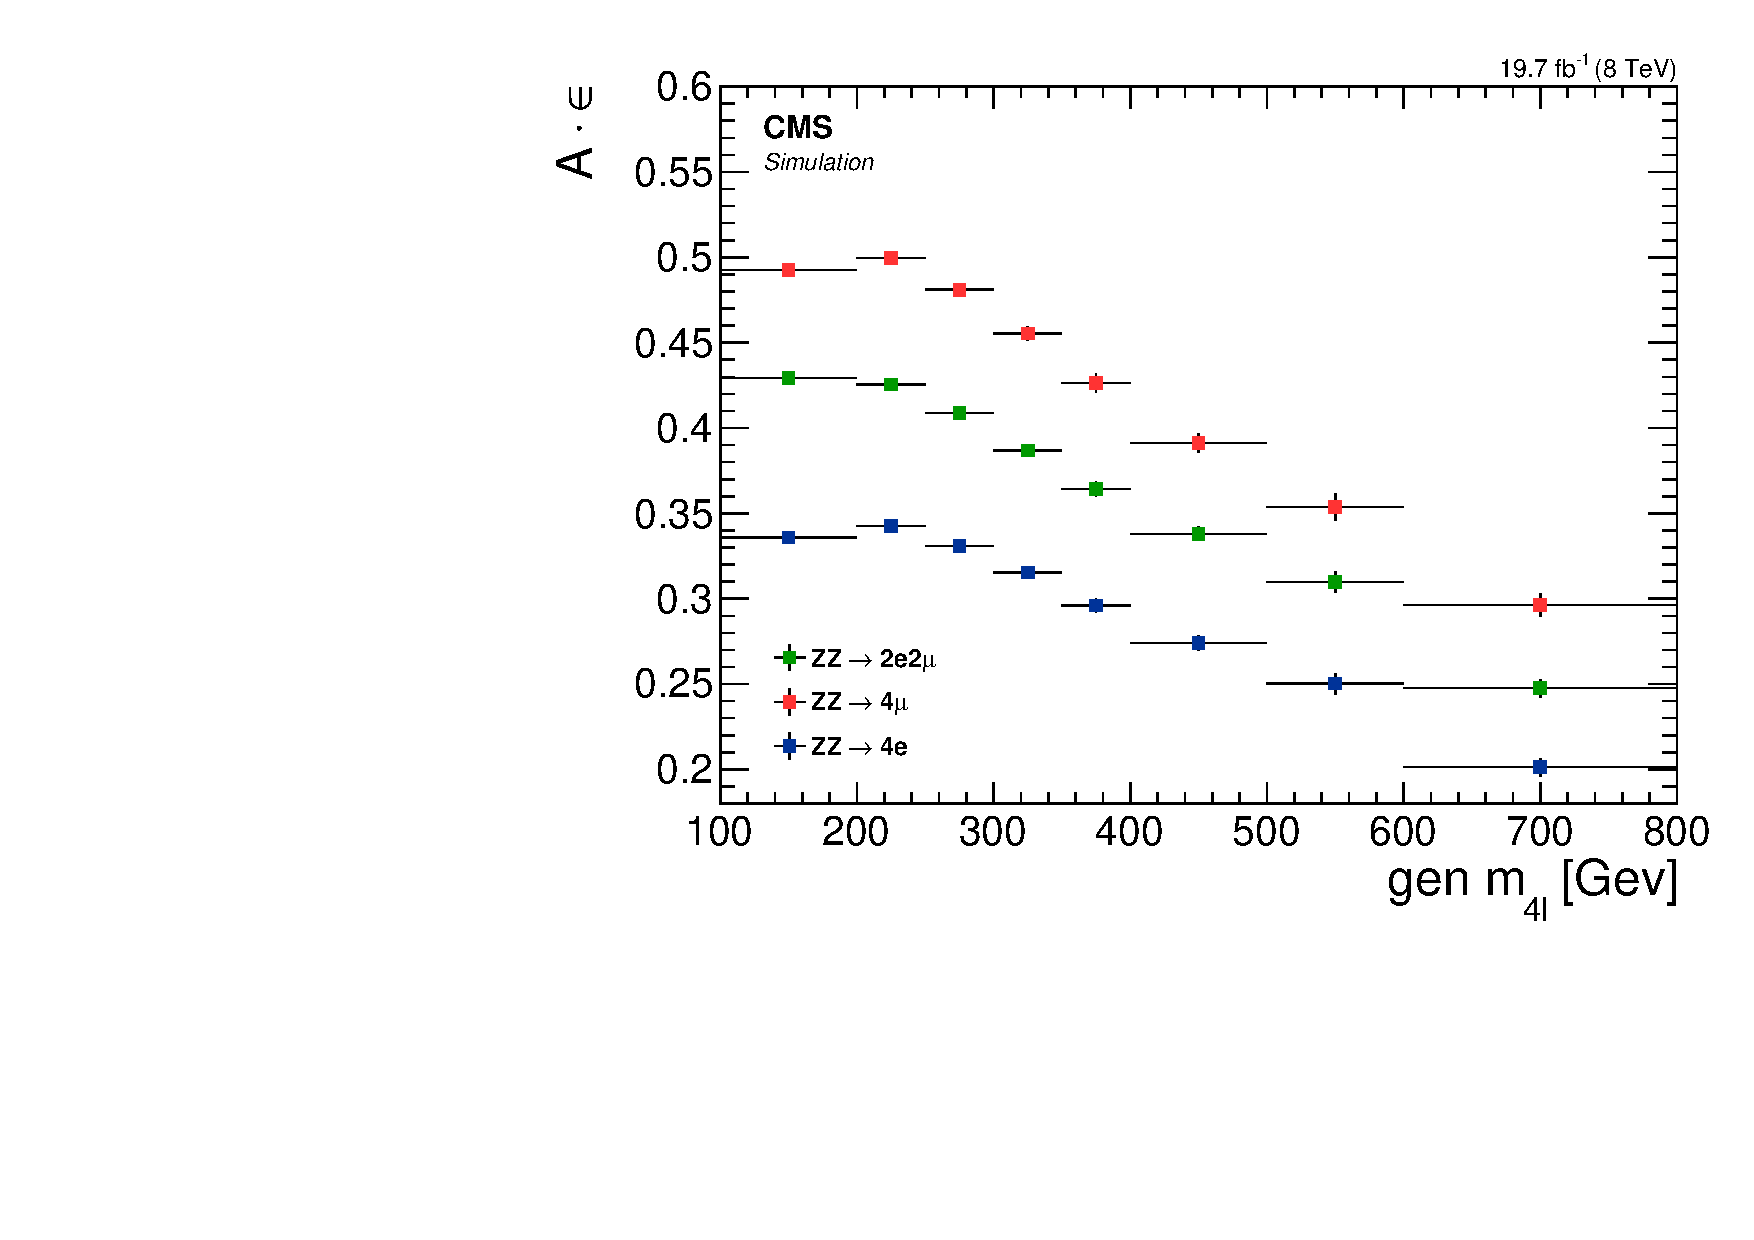
\includegraphics[width=\cmsFigWidth]{Figures/DiffAcceptance_Mass_Pow}
    
\includegraphics[width=\cmsFigWidth]{Figures/DiffAcceptance_Jets_Mad}
    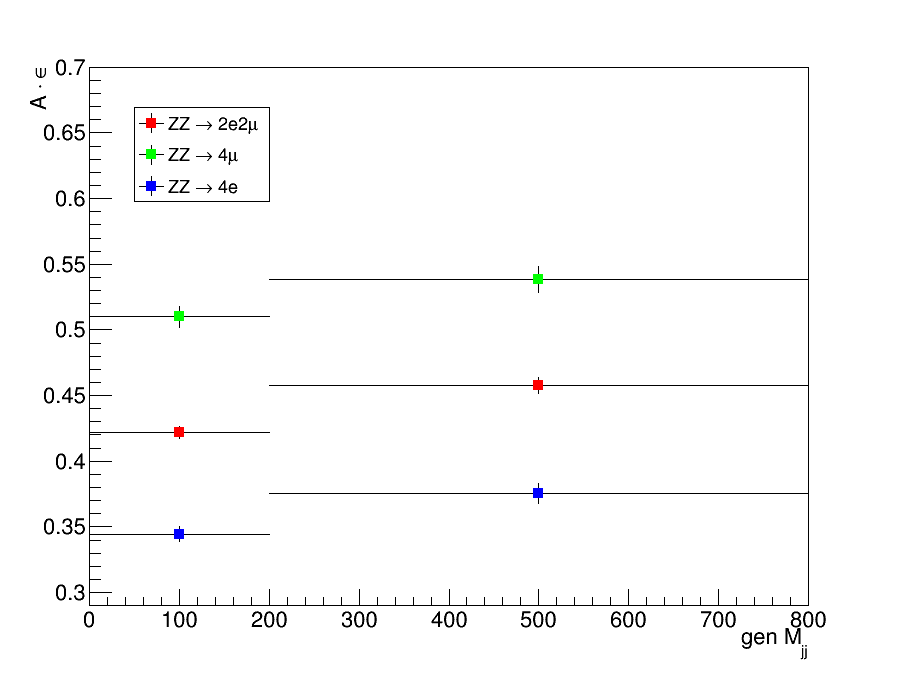
\includegraphics[width=\cmsFigWidth]{Figures/DiffAcceptance_Mjj_Mad}
    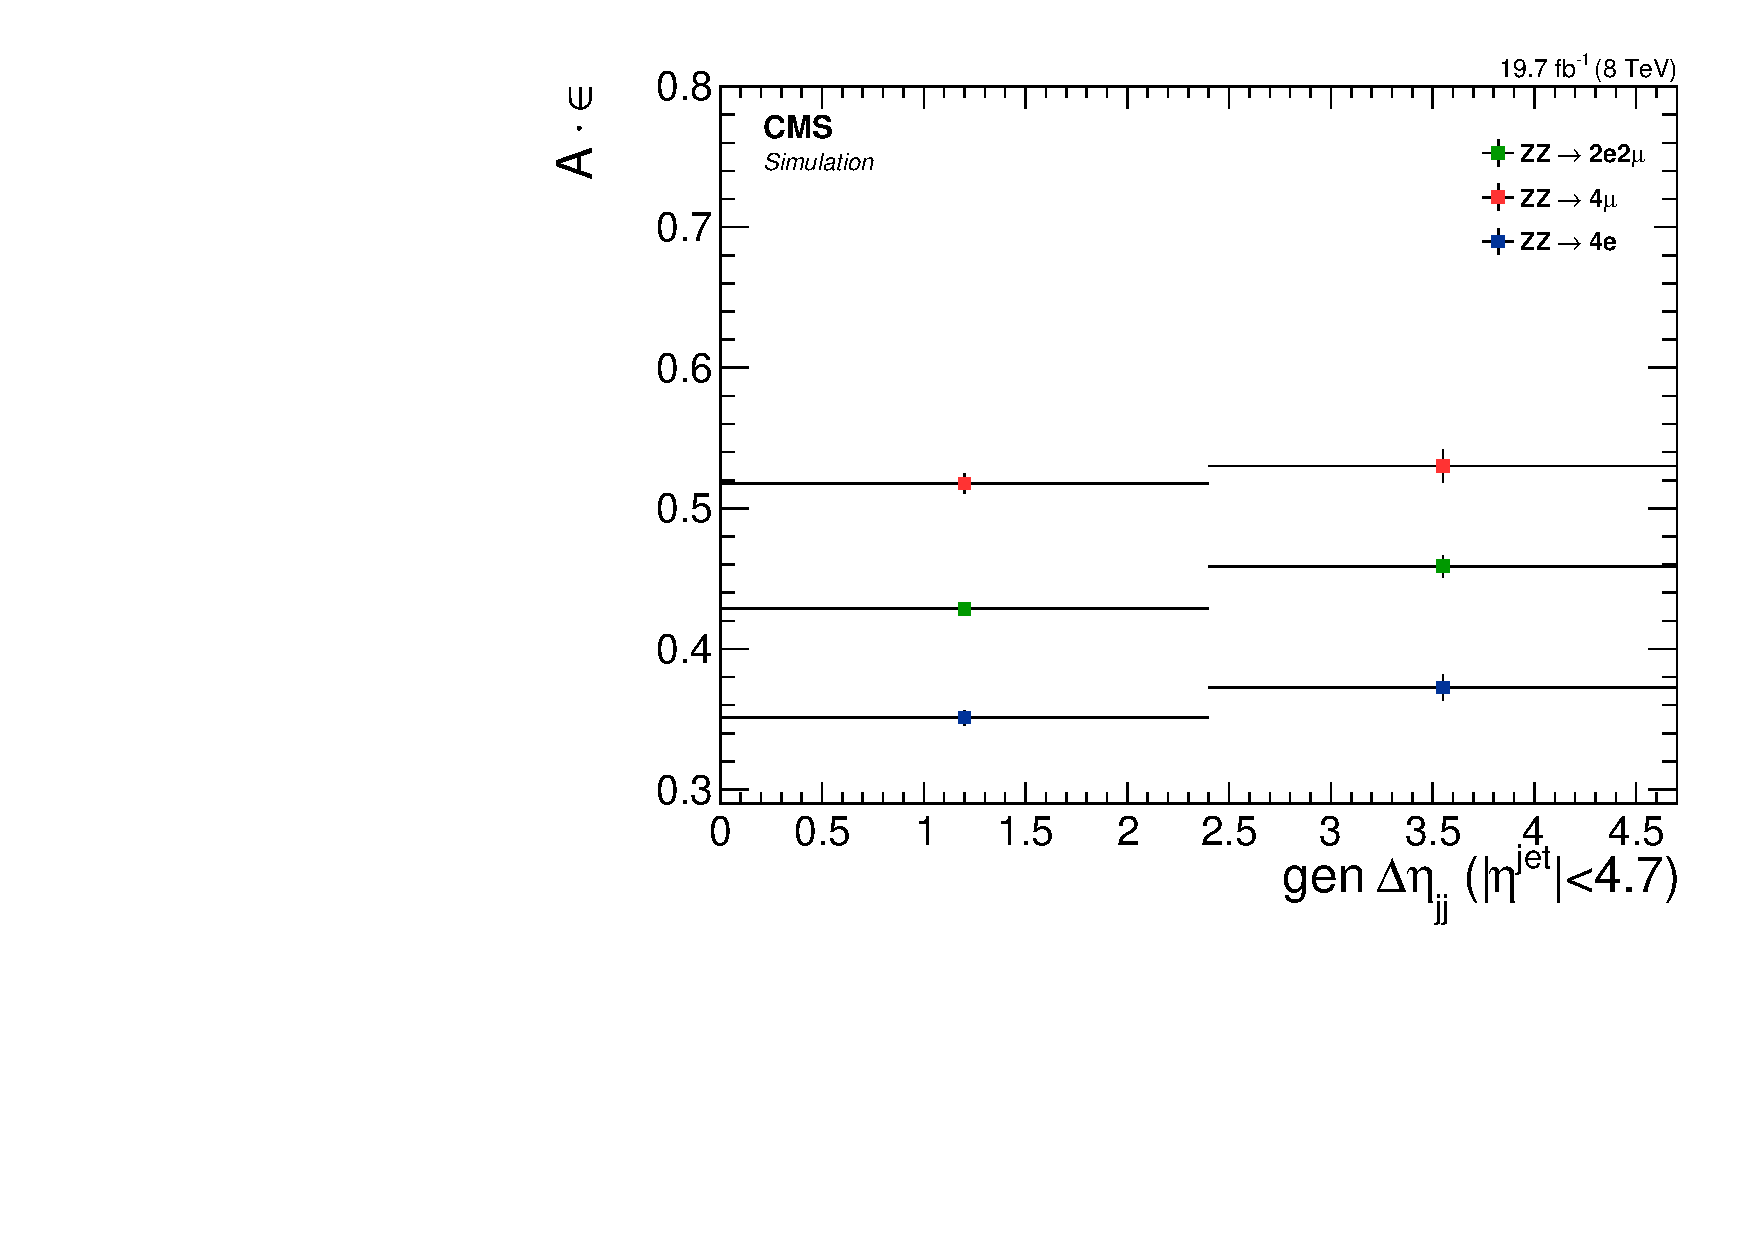
\includegraphics[width=\cmsFigWidth]{Figures/DiffAcceptance_Deta_Mad}
    %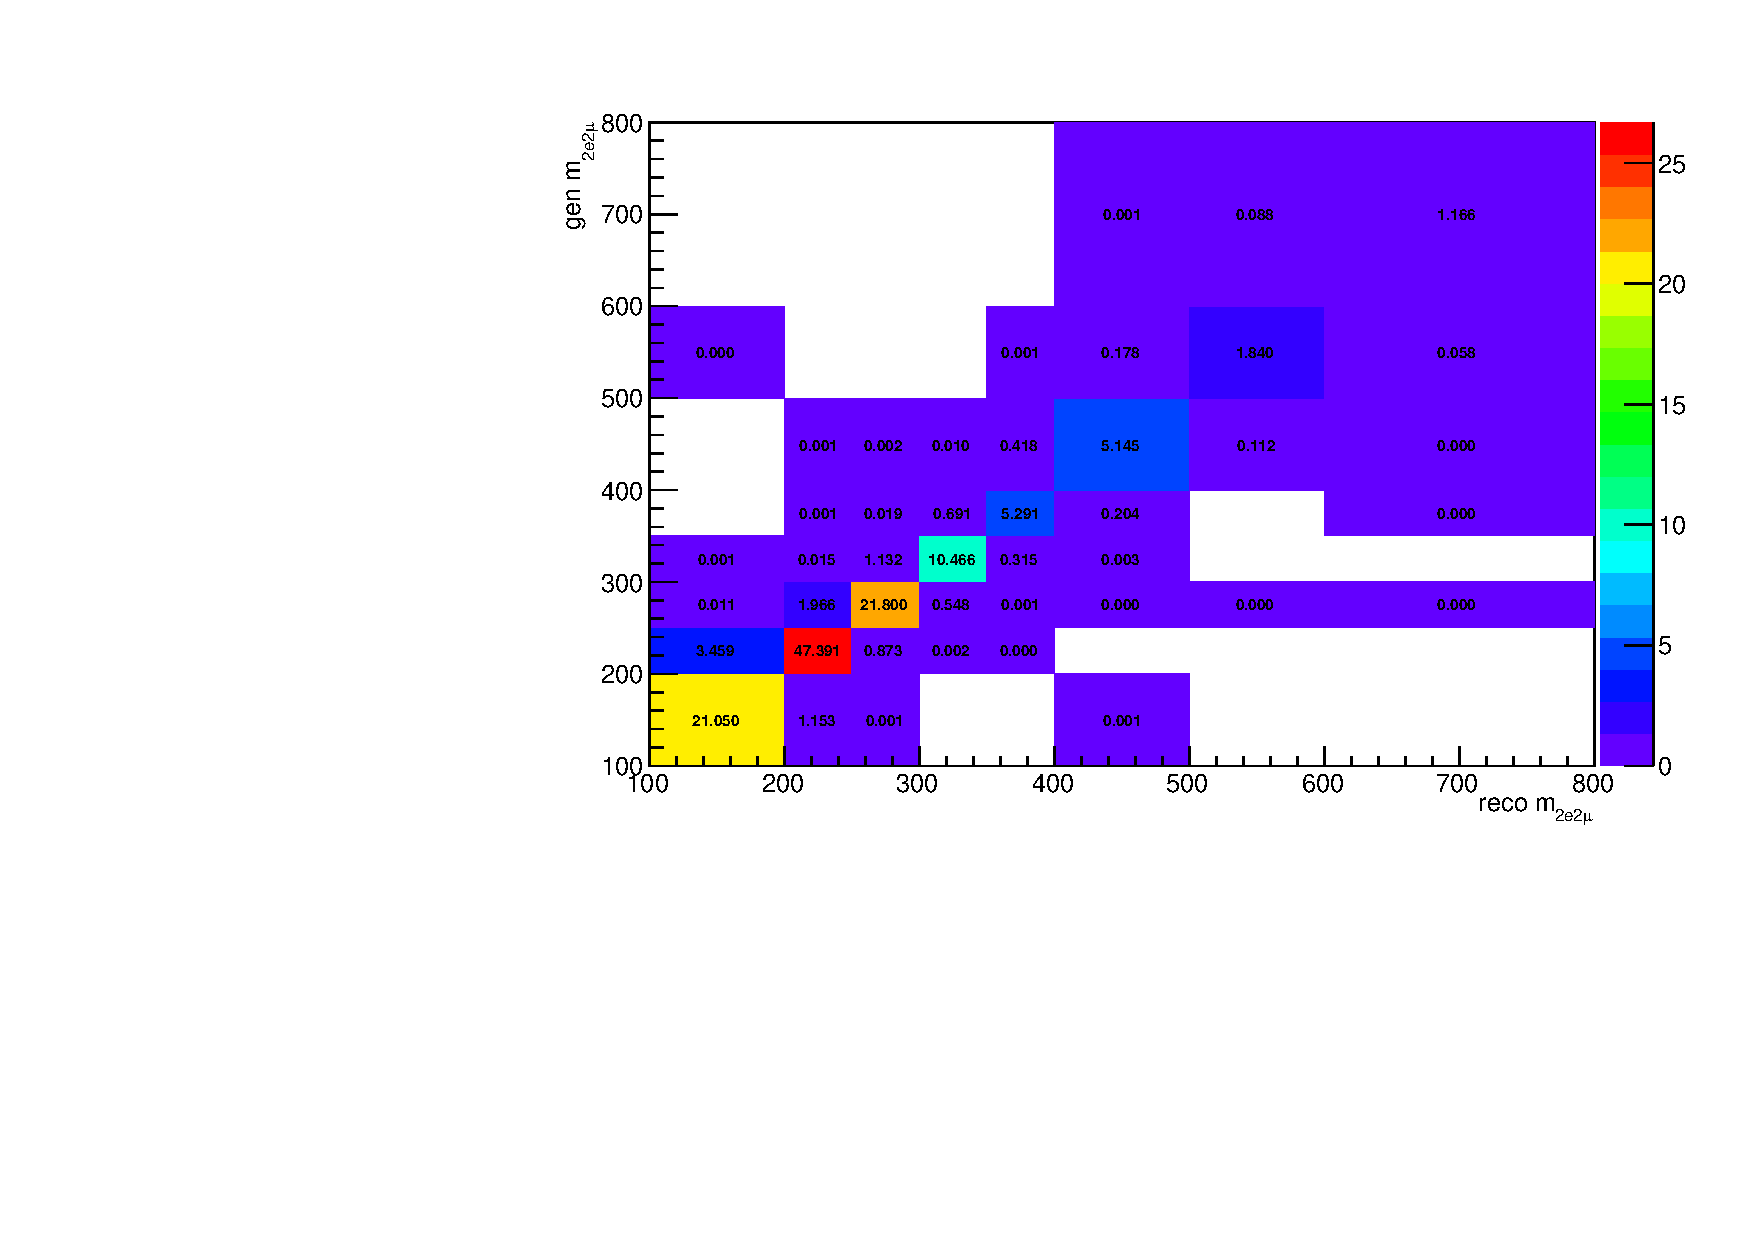
\includegraphics[width=\cmsFigWidth]{Figures/ResMat_qqggJJ_Mass_ZZTo2e2m_st_01_Pow}     
 %   to generate (a) and (b) labels under the figures, you can use subfloat, but this is not recommended: takes too much space
 %   \subfloat[]{
\includegraphics[width=0.2\textwidth]{CMS-bw-logo}}\subfloat[]{
\includegraphics[width=0.2\textwidth]{CMScol}}
    \caption{Acceptance ($A \cdot \epsilon$) computed in the wider fiducial region as a function of $m_{ZZ}$  (top left), $N\ jets$  (top right), $m_{jj}$ (bottom left) and $\Delta\eta_{jj}$
distributions, according to the final state: 
      $4\mu$ (green), $4e$ (blue), $2e2\mu$  (red). Distributions are obtained using the  \texttt{Powheg} set of samples for  $m_{ZZ}$ and 
     the  \texttt{MadGraph} set of samples for the other variables.} 
    \label{fig:A_diff}
  \end{center}
\end{figure}
\begin{figure}[hbtp]
  \begin{center}
    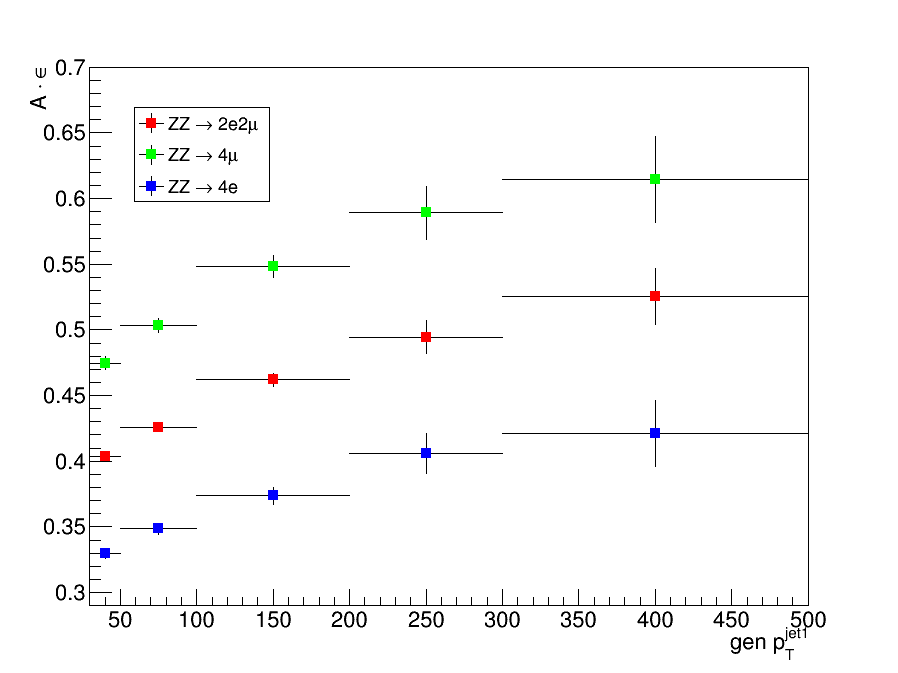
\includegraphics[width=\cmsFigWidth]{Figures/DiffAcceptance_PtJet1_Mad}
    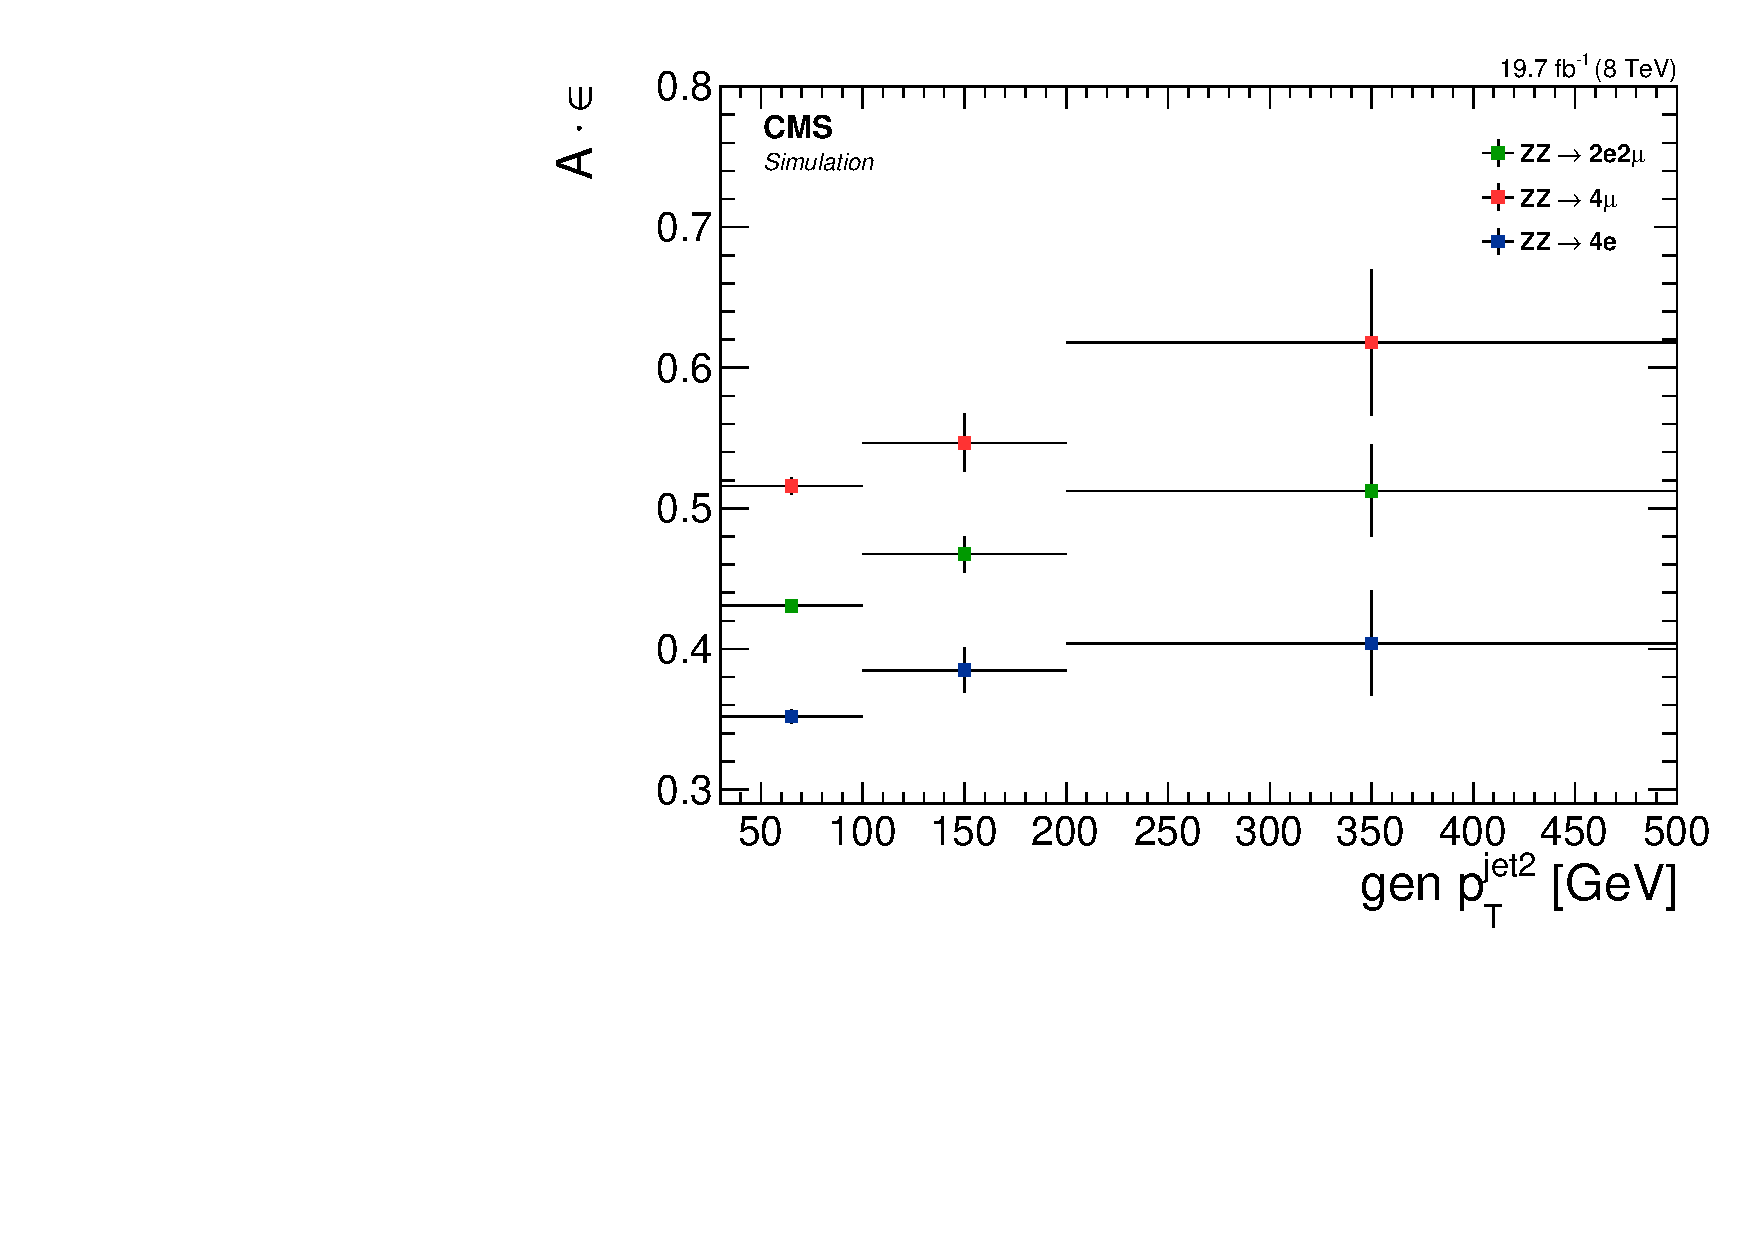
\includegraphics[width=\cmsFigWidth]{Figures/DiffAcceptance_PtJet2_Mad}
    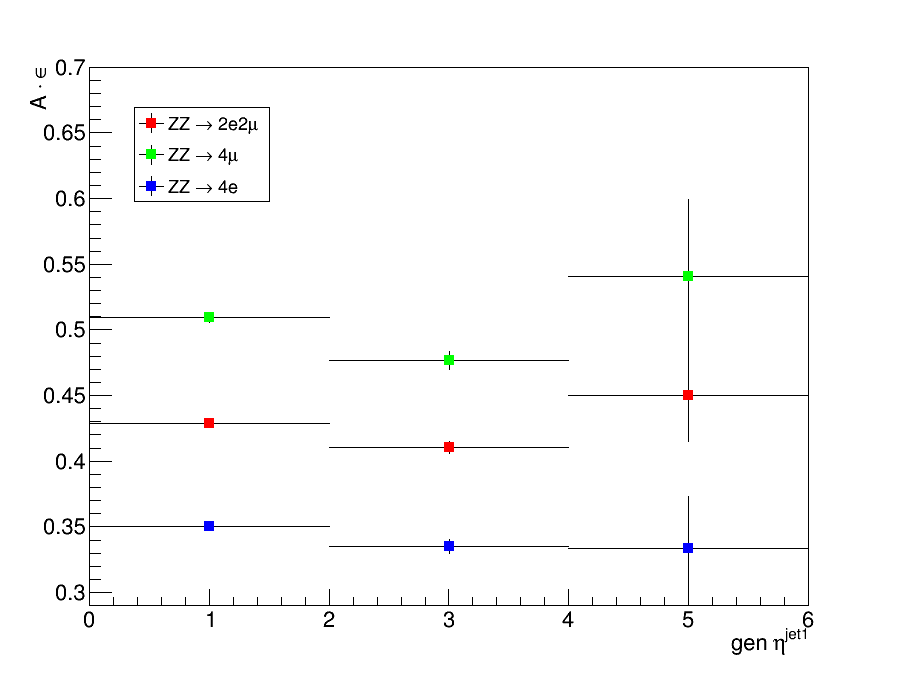
\includegraphics[width=\cmsFigWidth]{Figures/DiffAcceptance_EtaJet1_Mad}
    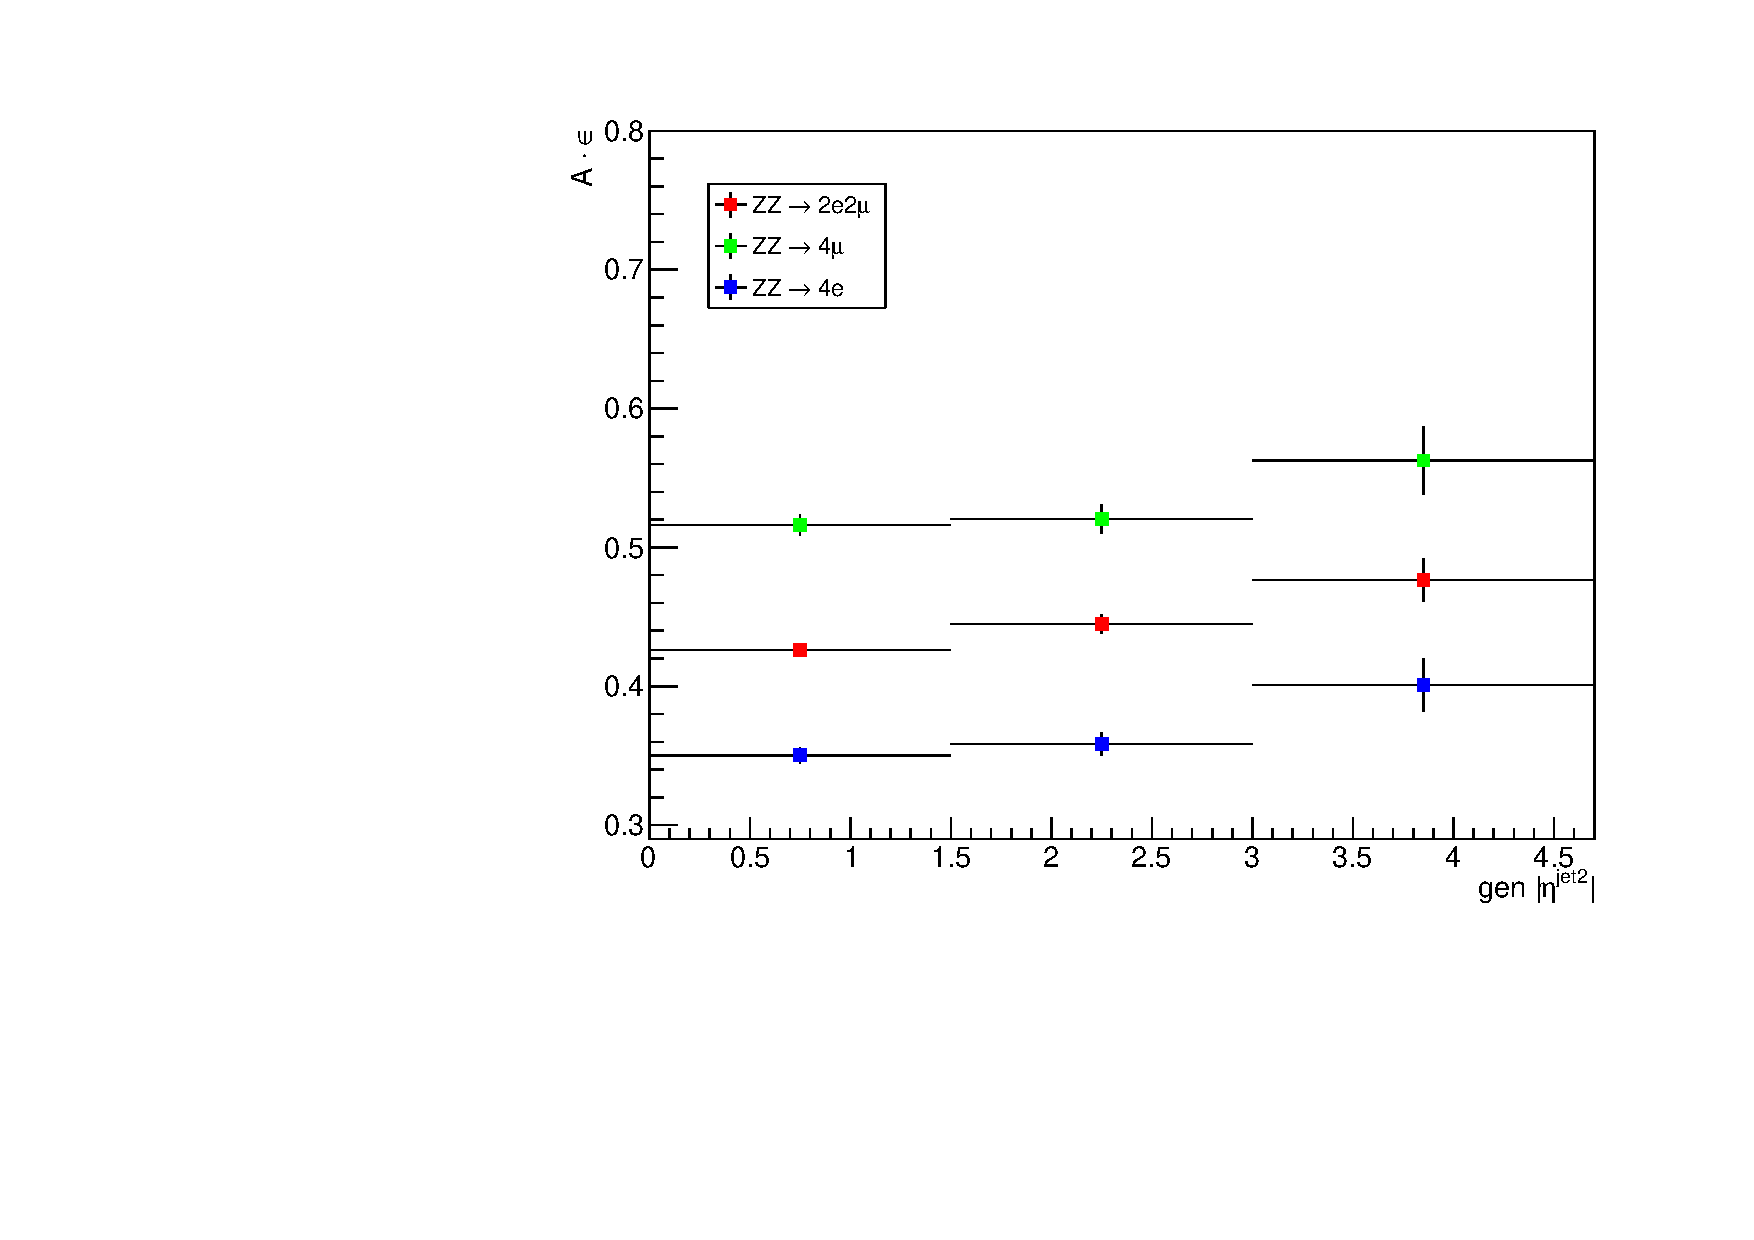
\includegraphics[width=\cmsFigWidth]{Figures/DiffAcceptance_EtaJet2_Mad}
    %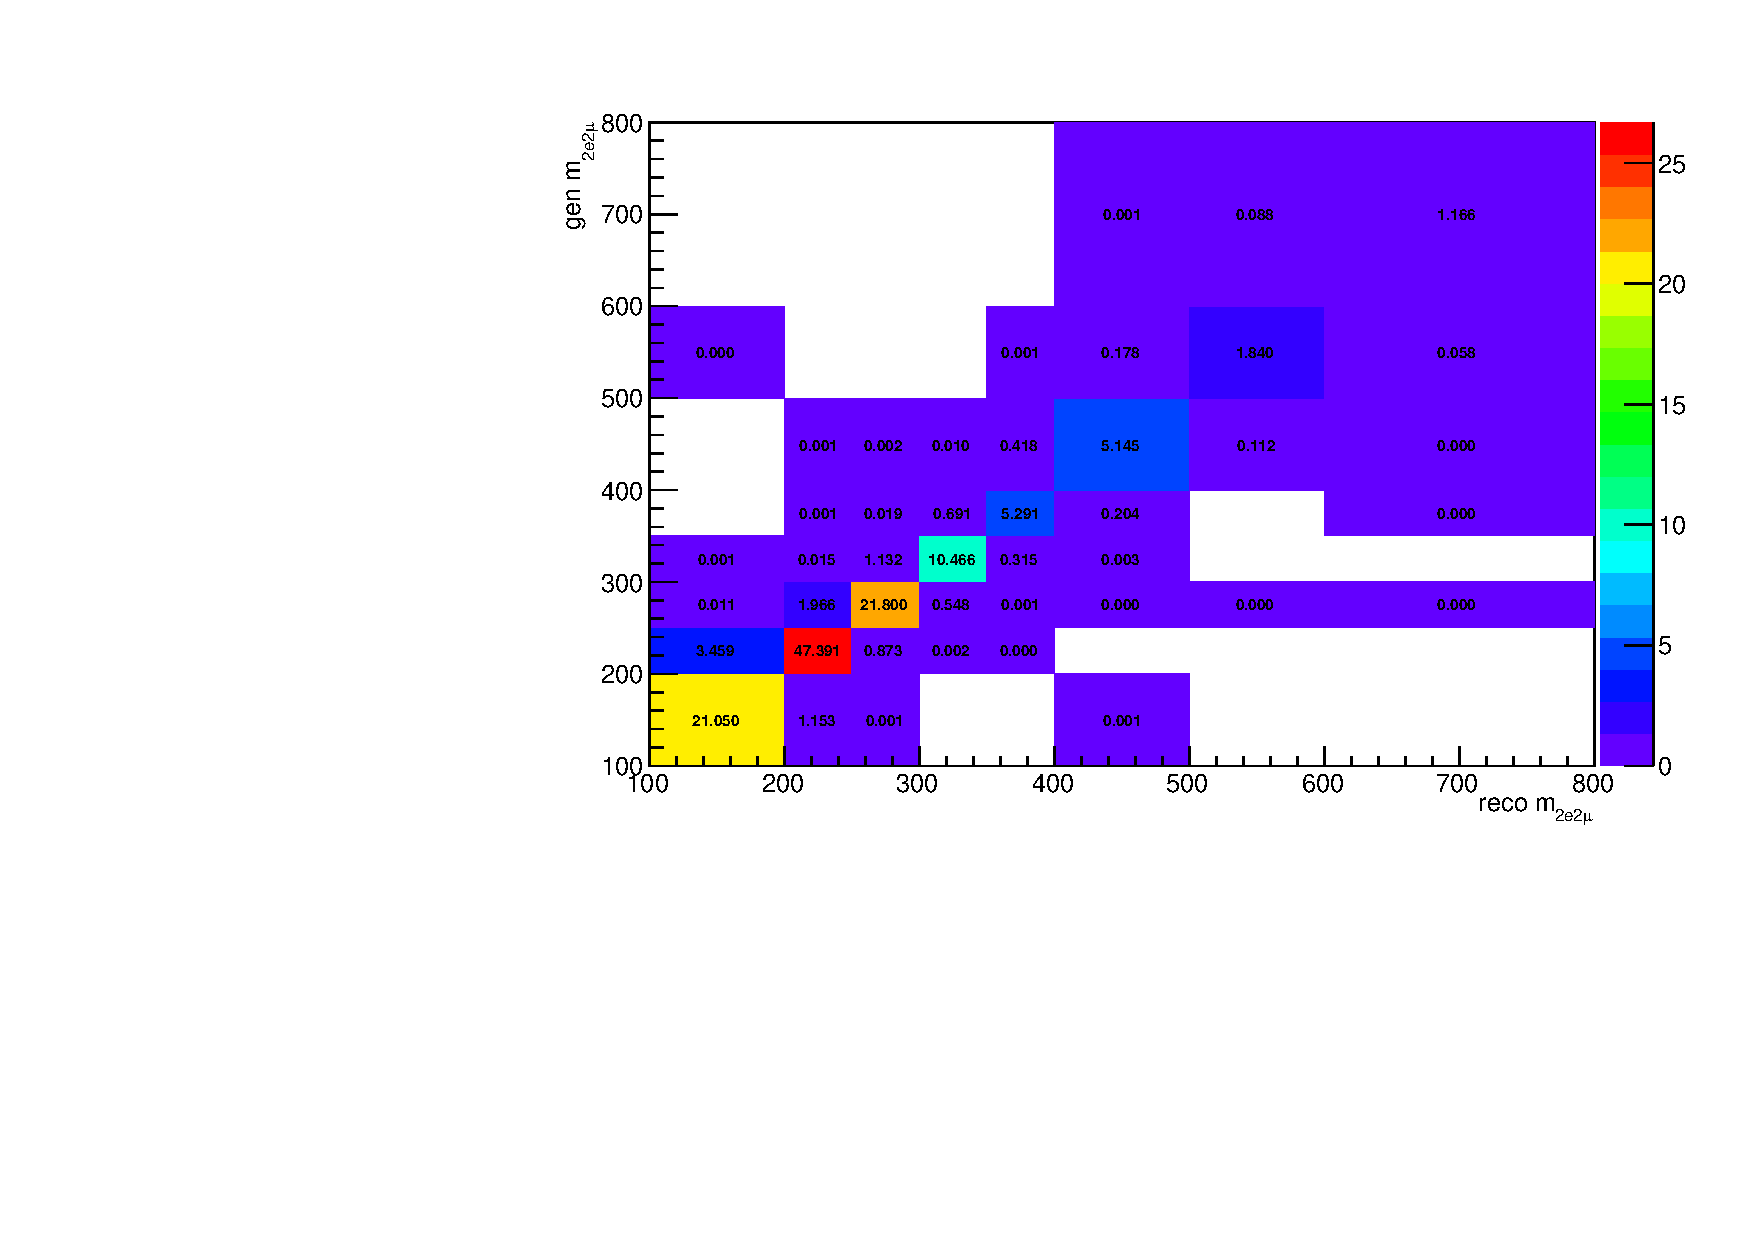
\includegraphics[width=\cmsFigWidth]{Figures/ResMat_qqggJJ_Mass_ZZTo2e2m_st_01_Pow}     
 %   to generate (a) and (b) labels under the figures, you can use subfloat, but this is not recommended: takes too much space
 %   \subfloat[]{
\includegraphics[width=0.2\textwidth]{CMS-bw-logo}}\subfloat[]{
\includegraphics[width=0.2\textwidth]{CMScol}}
    \caption{Acceptance ($A \cdot \epsilon$) computed in the wider fiducial region as a function of $p_T^{jet1}$  (top left), $p_T^{jet2}$  (top right), $\eta^{jet1}$ (bottom left) and $\eta^{jet2}$
distributions, according to the final state: 
      $4\mu$ (green), $4e$ (blue), $2e2\mu$  (red). Distributions are obtained using the  \texttt{Powheg} set of samples for  $m_{ZZ}$ and 
     the  \texttt{MadGraph} set of samples for the other variables.} 
    \label{fig:A_diff_jet}
  \end{center}
\end{figure}

\subsection{The differential ZZ cross-section measurements}
The study of vector boson pair production is important both as check of the SM and in search for new physics. 
Non-resonant $ZZ$ events are the dominant background in the $H \to ZZ \to 4\ell$ analysis and a good knowledge of 
these processes is  very useful for the study of the associated production of a $Z$ boson with the Higgs, especially at 13 TeV.
However, a lot of information
can still be extracted from data at 8 TeV, in particular as regards the associate production of a Z boson pair with jets. 
In addiction to the invariant mass of the four lepton system, the differential $ZZ$ cross-section is determined as
a function of the number of jets produced in the event, the invariant mass of the two most energetic jets ($m_{jj}$), the 
$\Delta\eta$ between them ($\Delta\eta_{jj}$), their transverse momentum and pseudorapidity (leading jet $p_{T}(\eta)^{jet1}$ and sub-leading jet $p_{T}(\eta)^{jet2}$). Both jets with  $\eta^{jet}<4.7$ and central jets with $\eta^{jet}<2.4$ are considered.\\
\\
The cross-section in each bin of each observable is determined from the event yields subtracting
the backgrounds. Each distribution is then corrected for event selection efficiencies
and for detector resolution effects in order to be compared with predictions from event generators.
The correction procedure is based on unfolding techniques, as implemented in the
\texttt{RooUnfold} toolkit~\cite{RooUnfold}, which provides both singular value decomposition (SVD)~\cite{SVD} and
the d'Agostini~\cite{DAgostini} methods. Both algorithms use a response matrix that correlates the observable
with and without detector effects. Regularization parameters can be tuned to obtain results that are robust against 
numerical instabilities and statistical fluctuations. The differential cross-section is then derived by dividing the
corrected number of events by the integrated luminosity, the branching ratio and the bin width.\\
\\
For each measured distribution, a response matrix is evaluated using two different sets of generators: the first one is composed of signal samples generated with \texttt{MadGraph} ($qq/qg/gg \to ZZ$), \texttt{MCFM} ($gg \to ZZ$) and \texttt{Phantom} ($qq \to ZZ+2jets$). The second one has the \texttt{Powheg} sample ($qq \to ZZ$) instead of
the \texttt{MadGraph} one. The \texttt{MadGraph} set is the reference set for the jet-related variables,
while the  \texttt{Powheg} one is used for check and comparison purposes. For the $m_{ZZ}$ distribution the role of the two sets of samples is switched.\\
As reported above, the signal definition of the generated events requires $60 < m_{Z_1}, m_{Z_2} < 120$  GeV. 
%  and $m_{ZZ} >$ 100 GeV. 
In order to minimize the model uncertainties due to unnecessary extrapolations of the measurement outside experimentally well-described phase space regions, cross-section distributions are also extracted in the tighter fiducial region, corresponding to the visible phase space defined by the kinematic and geometrical acceptance of leptons.\\ 
The same selection as in the inclusive cross-section measurement is applied to the reconstructed events.\\ 
Response matrices built using the reference set of samples and obtained in the tight fiducial region are 
reported in Figures~\ref{fig:Mass_matrices}-%,~\ref{fig:Jets_matrices},~\ref{fig:CentralJets_matrices},~\ref{fig:Mjj_matrices},~\ref{fig:Mjj_matrices},~\ref{fig:Deta_matrices},~\ref{fig:CentralDeta_matrices},~\ref{fig:PtJet1_matrices} and
\ref{fig:PtJet2_matrices} for each variable.\\
\begin{figure}[hbtp]
  \begin{center}
    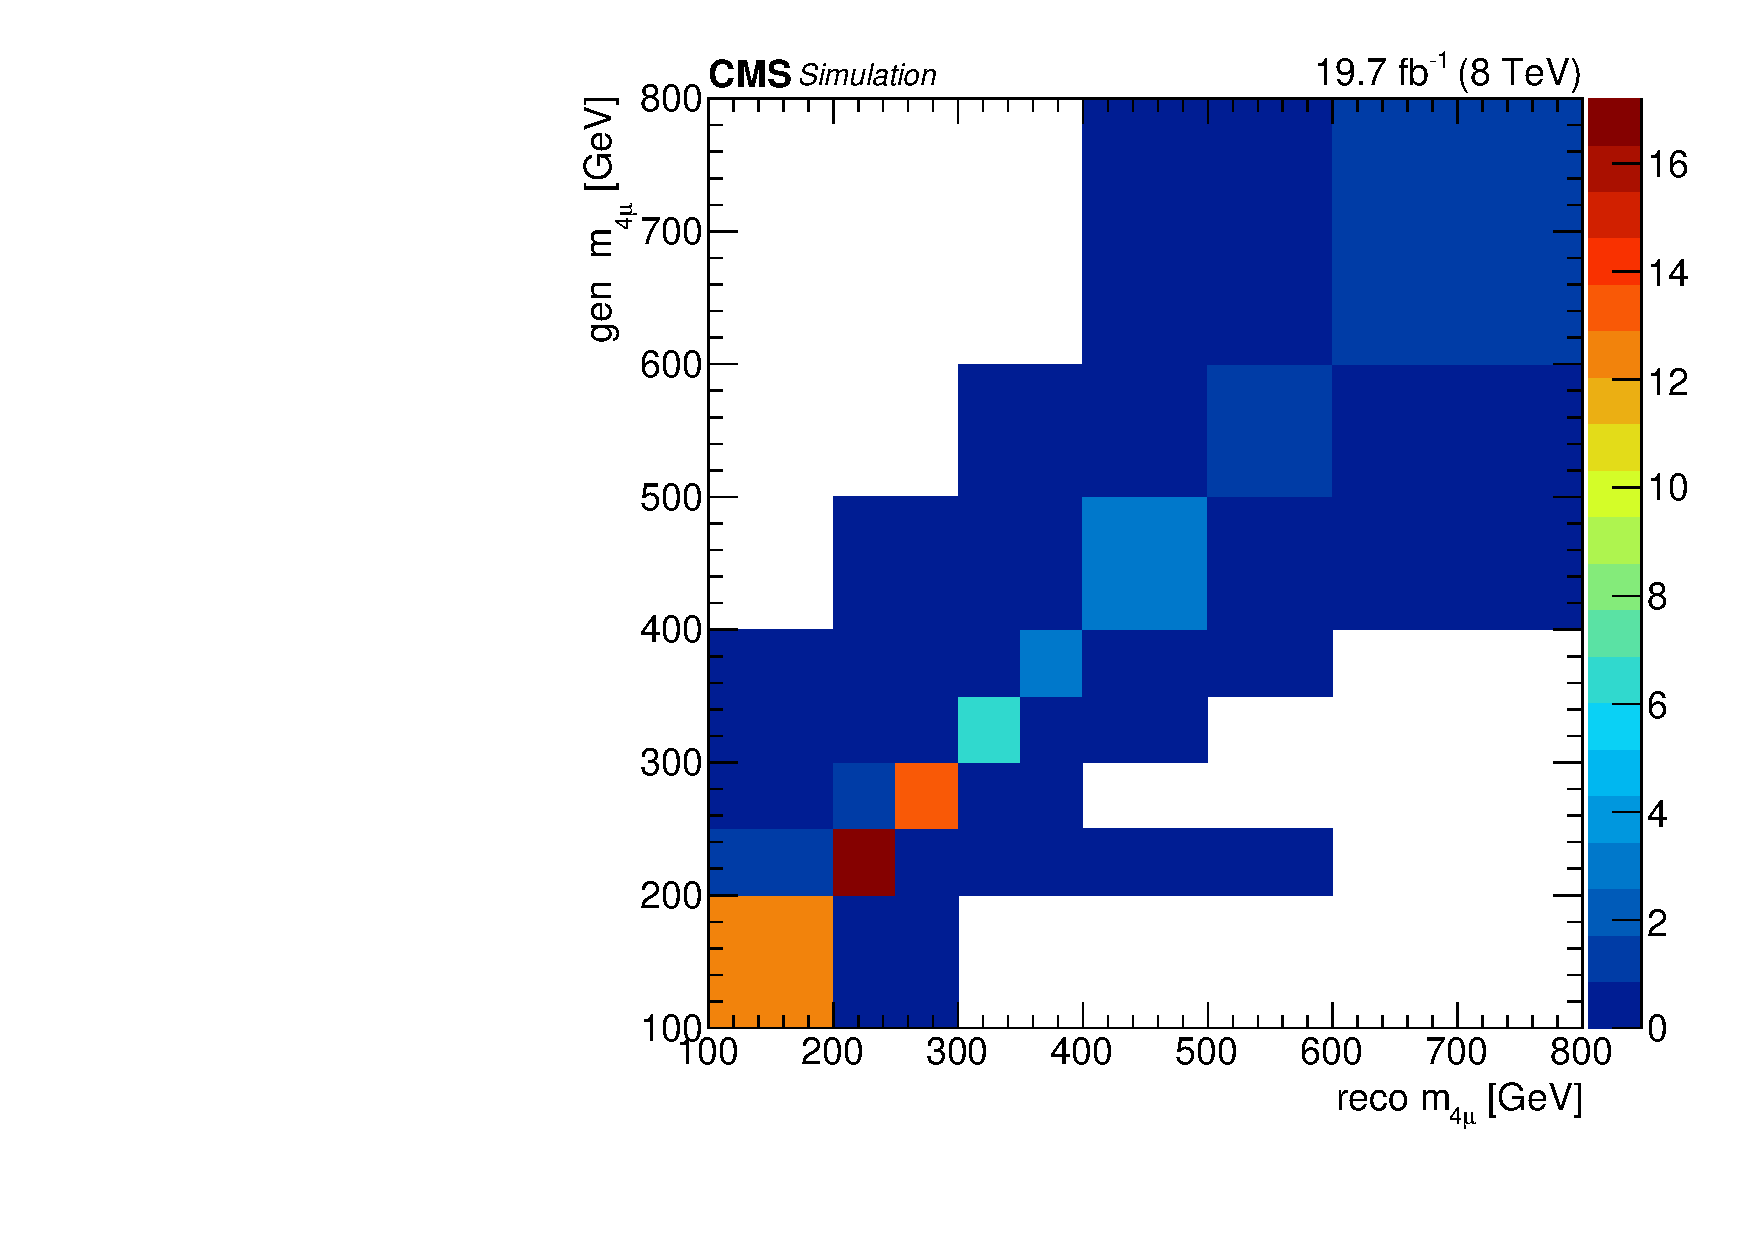
\includegraphics[width=\cmsFigWidth]{Figures/ResMat_qqggJJ_Mass_ZZTo4m_st_01_fr_Pow}
    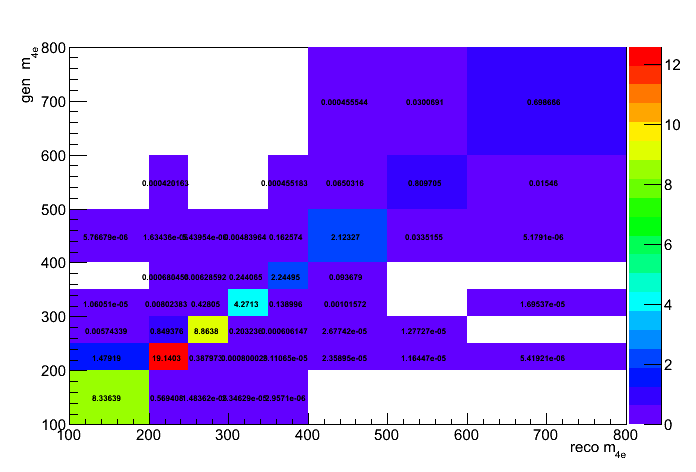
\includegraphics[width=\cmsFigWidth]{Figures/ResMat_qqggJJ_Mass_ZZTo4e_st_01_fr_Pow}
    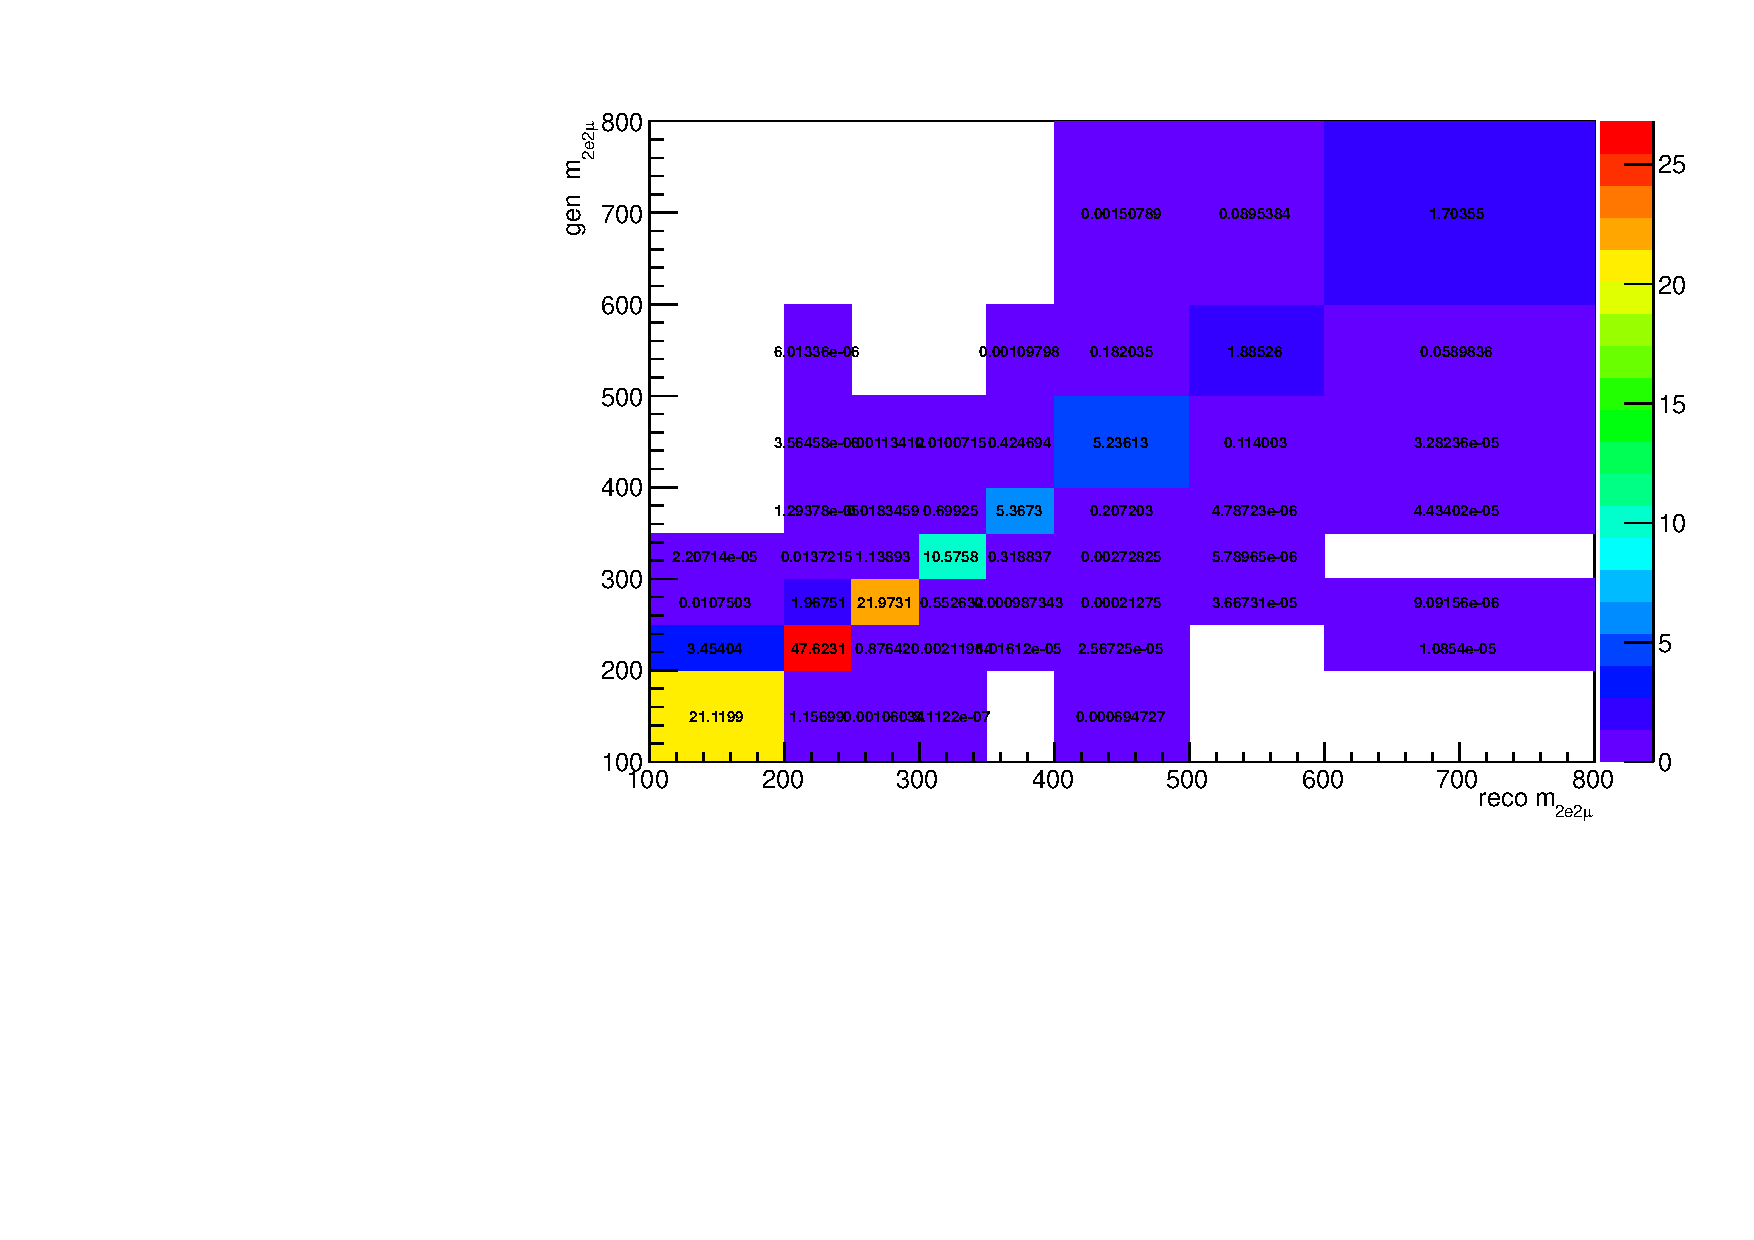
\includegraphics[width=\cmsFigWidth]{Figures/ResMat_qqggJJ_Mass_ZZTo2e2m_st_01_fr_Pow}     
 %   to generate (a) and (b) labels under the figures, you can use subfloat, but this is not recommended: takes too much space
 %   \subfloat[]{
\includegraphics[width=0.2\textwidth]{CMS-bw-logo}}\subfloat[]{
\includegraphics[width=0.2\textwidth]{CMScol}}
    \caption{Response matrices for the $m_{ZZ}$ distribution, according to the final state:  $4\mu$ (top left), $4e$ (top right), $2e2\mu$  (bottom). Matrices are obtained using the  \texttt{Powheg} set of samples. The tight fiducial region is considered.} 
    \label{fig:Mass_matrices}
  \end{center}
\end{figure}

\begin{figure}[hbtp]
  \begin{center}
    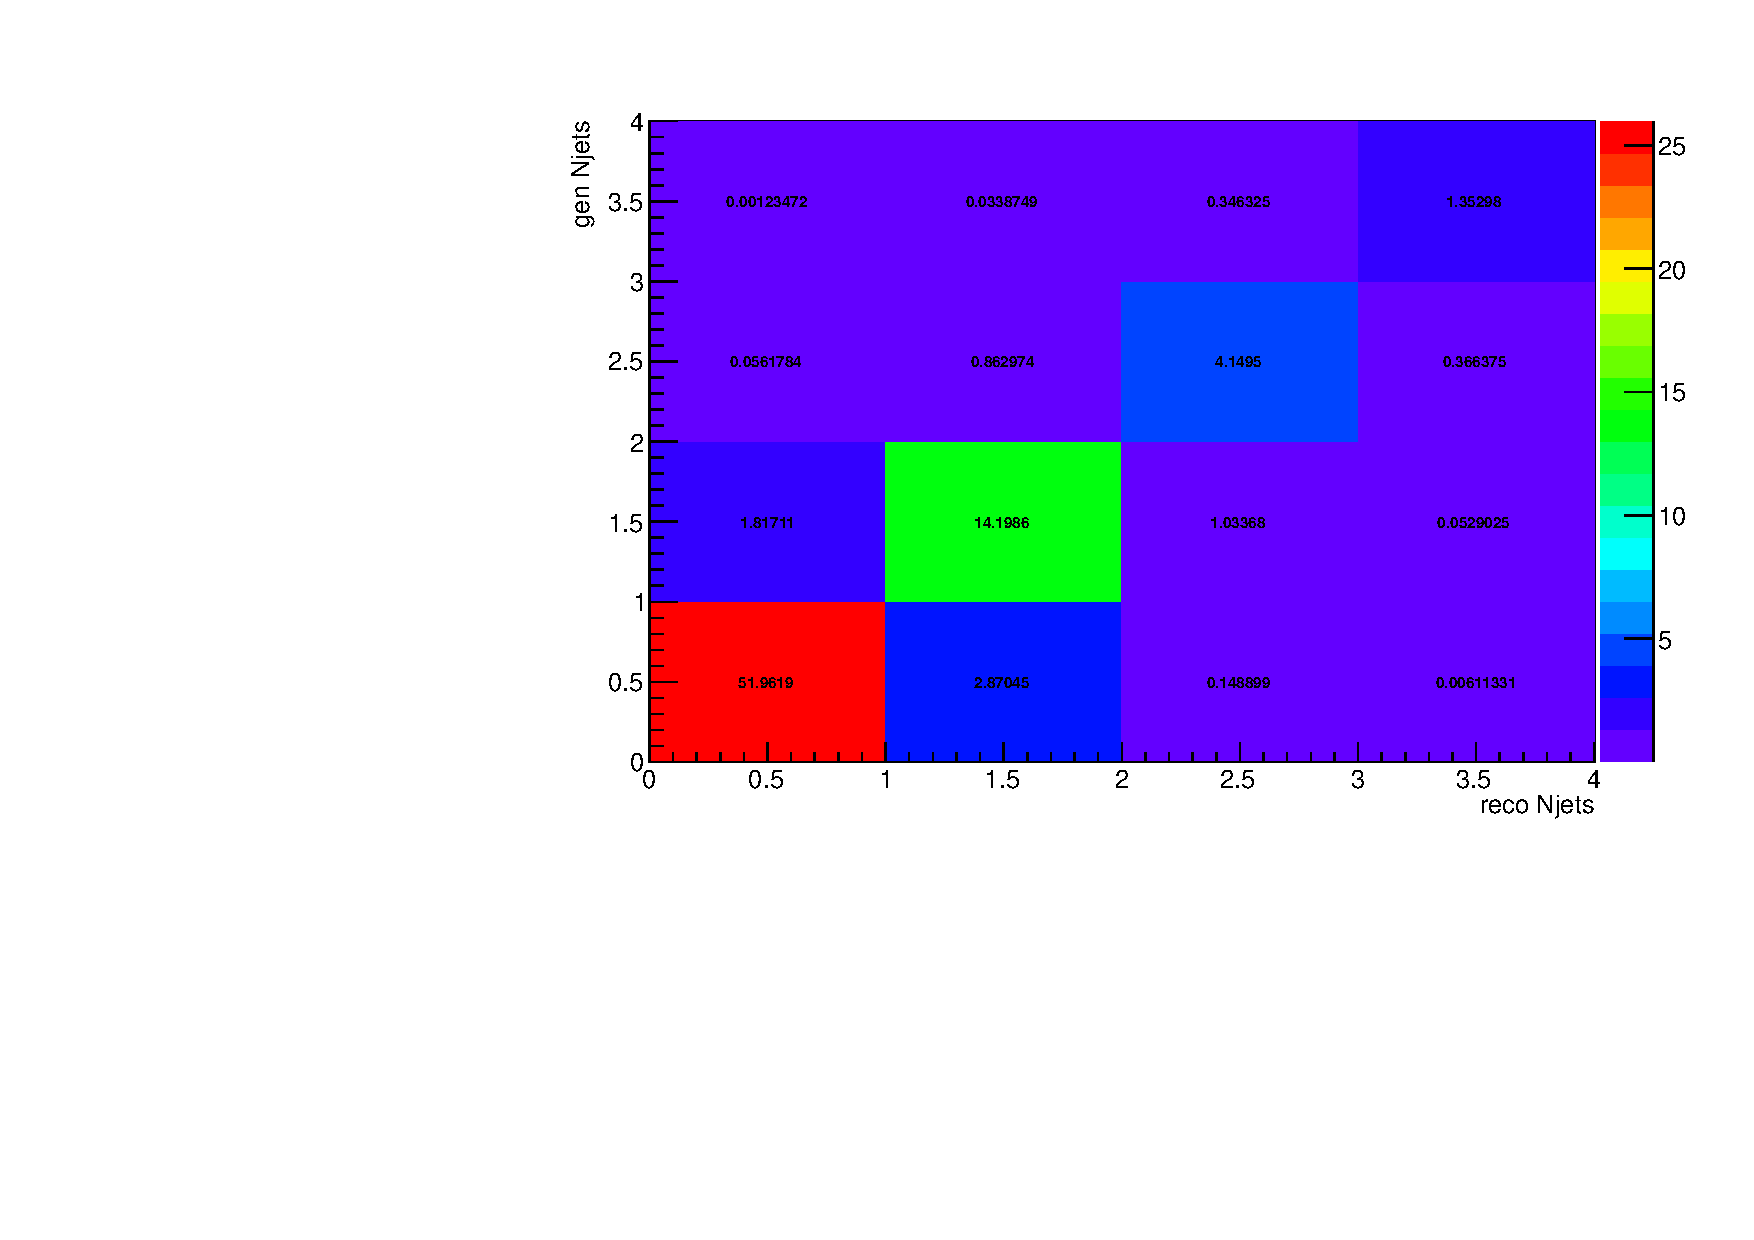
\includegraphics[width=\cmsFigWidth]{Figures/ResMat_qqggJJ_Jets_ZZTo4m_st_01_fr_Mad}
    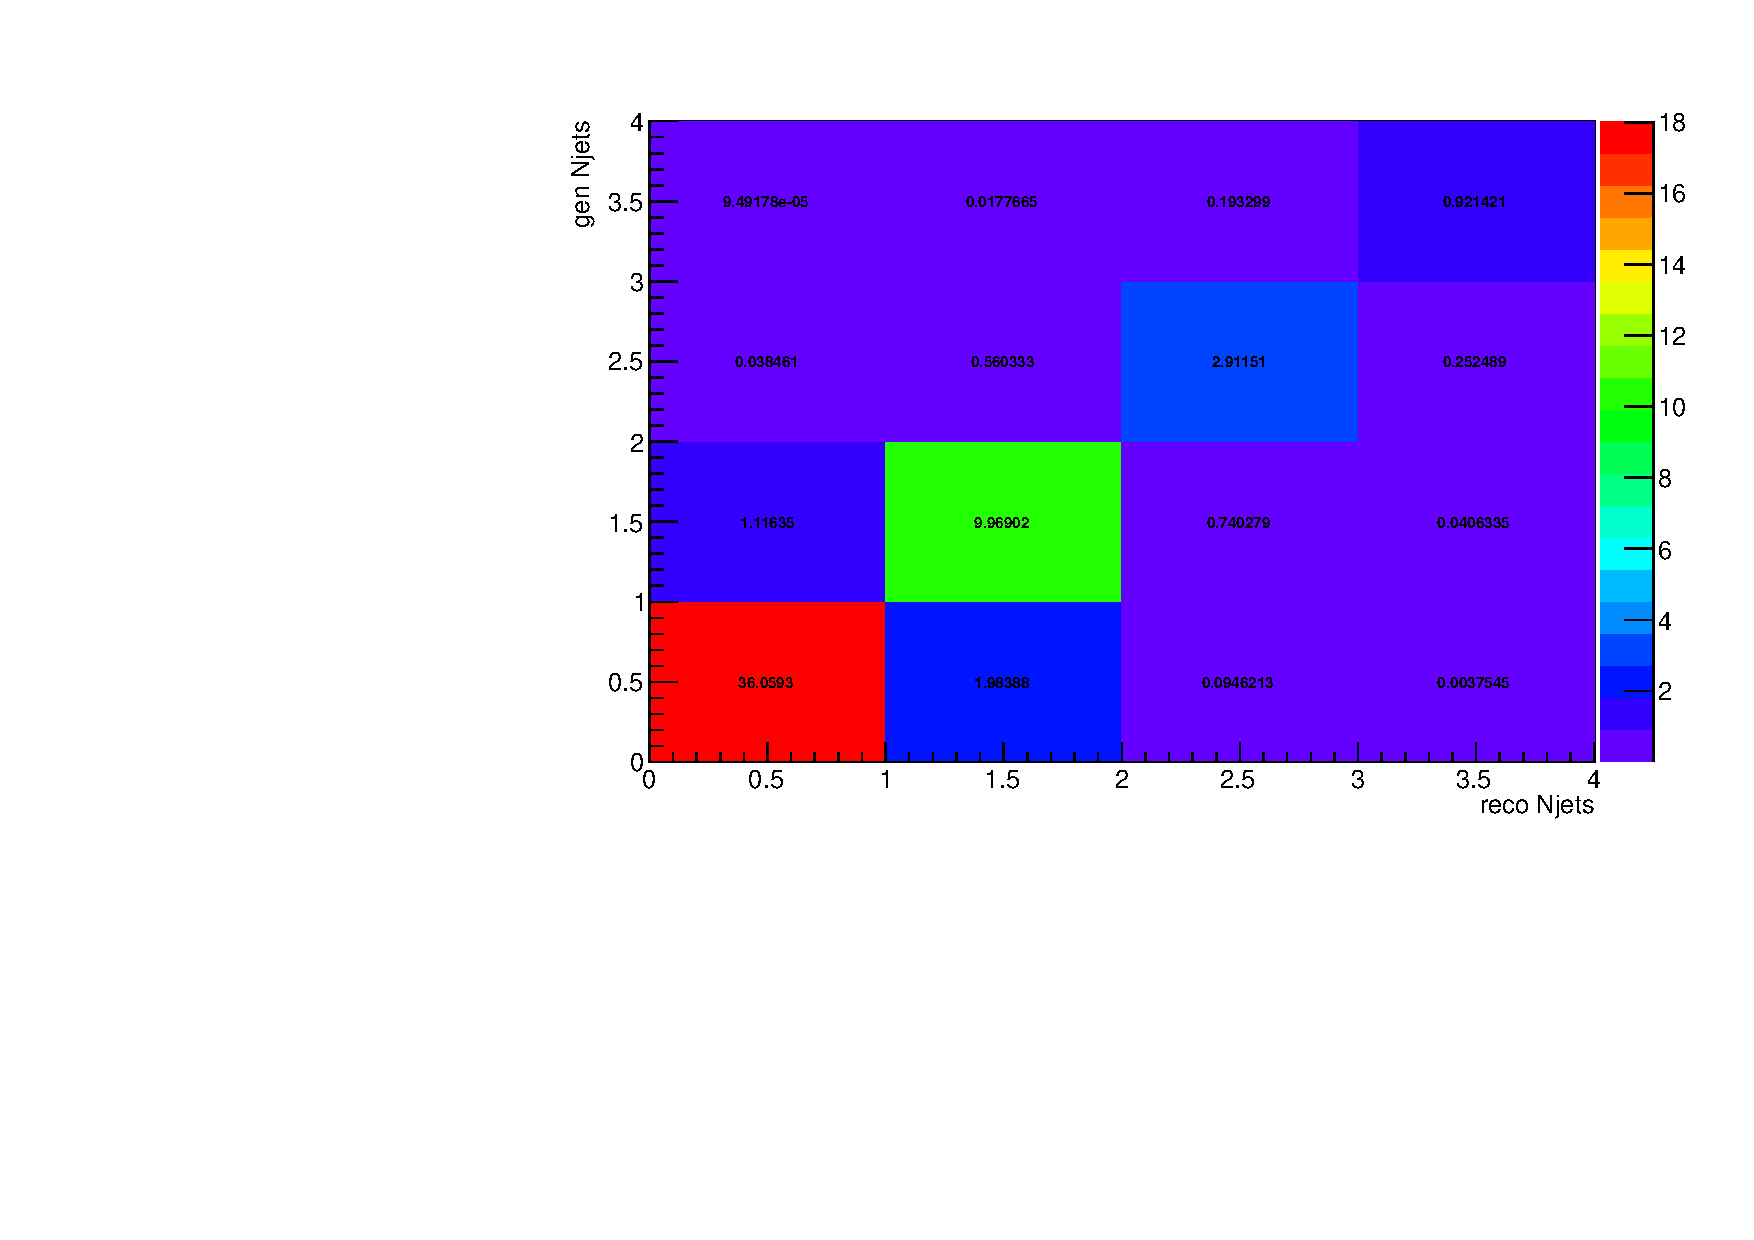
\includegraphics[width=\cmsFigWidth]{Figures/ResMat_qqggJJ_Jets_ZZTo4e_st_01_fr_Mad}
    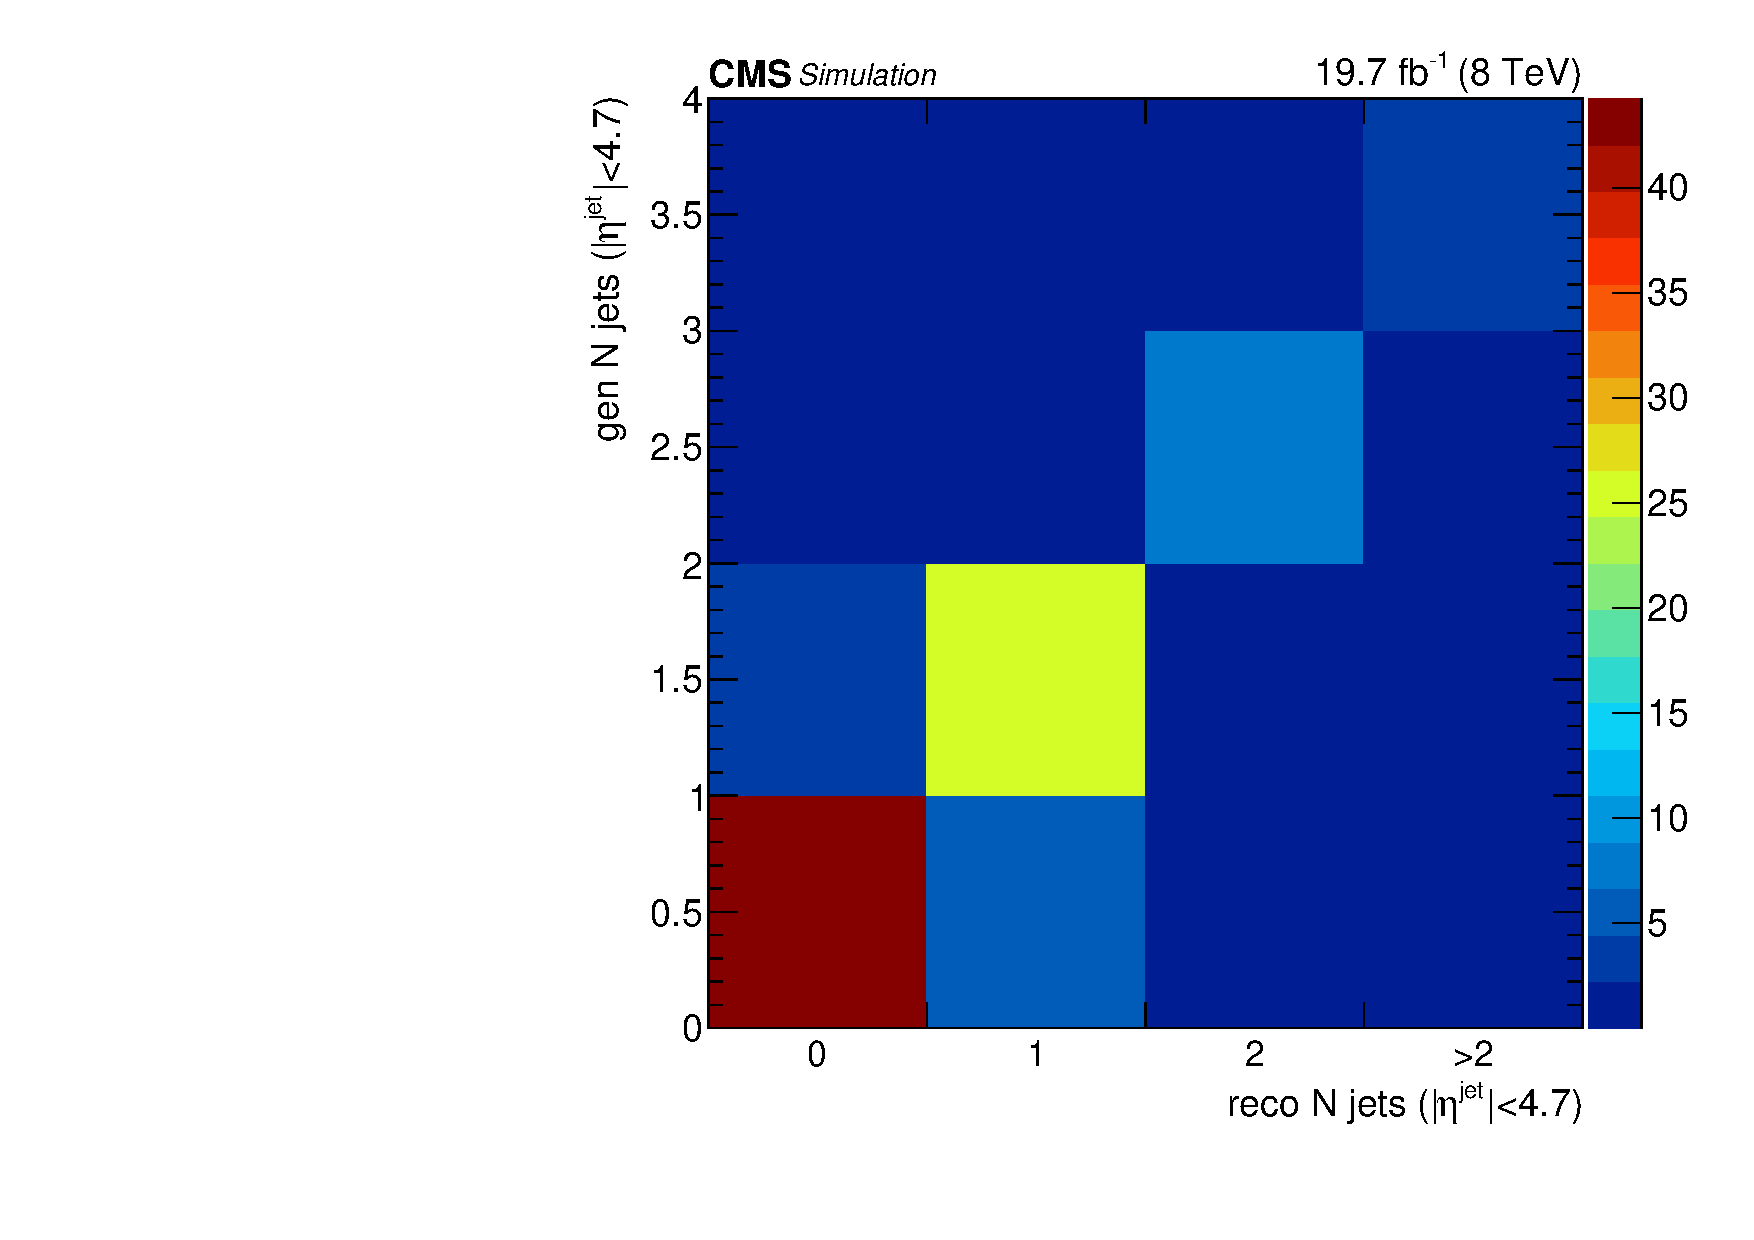
\includegraphics[width=\cmsFigWidth]{Figures/ResMat_qqggJJ_Jets_ZZTo2e2m_st_01_fr_Mad}     
 %   to generate (a) and (b) labels under the figures, you can use subfloat, but this is not recommended: takes too much space
 %   \subfloat[]{
\includegraphics[width=0.2\textwidth]{CMS-bw-logo}}\subfloat[]{
\includegraphics[width=0.2\textwidth]{CMScol}}
    \caption{Response matrices for the $N\ jets$ distribution, according to the final state:  $4\mu$ (top left), $4e$ (top right), $2e2\mu$  (bottom). Matrices are obtained using the  \texttt{MadGraph} set of samples. The tight fiducial region is considered.} 
    \label{fig:Jets_matrices}
  \end{center}
\end{figure}
\begin{figure}[hbtp]
  \begin{center}
    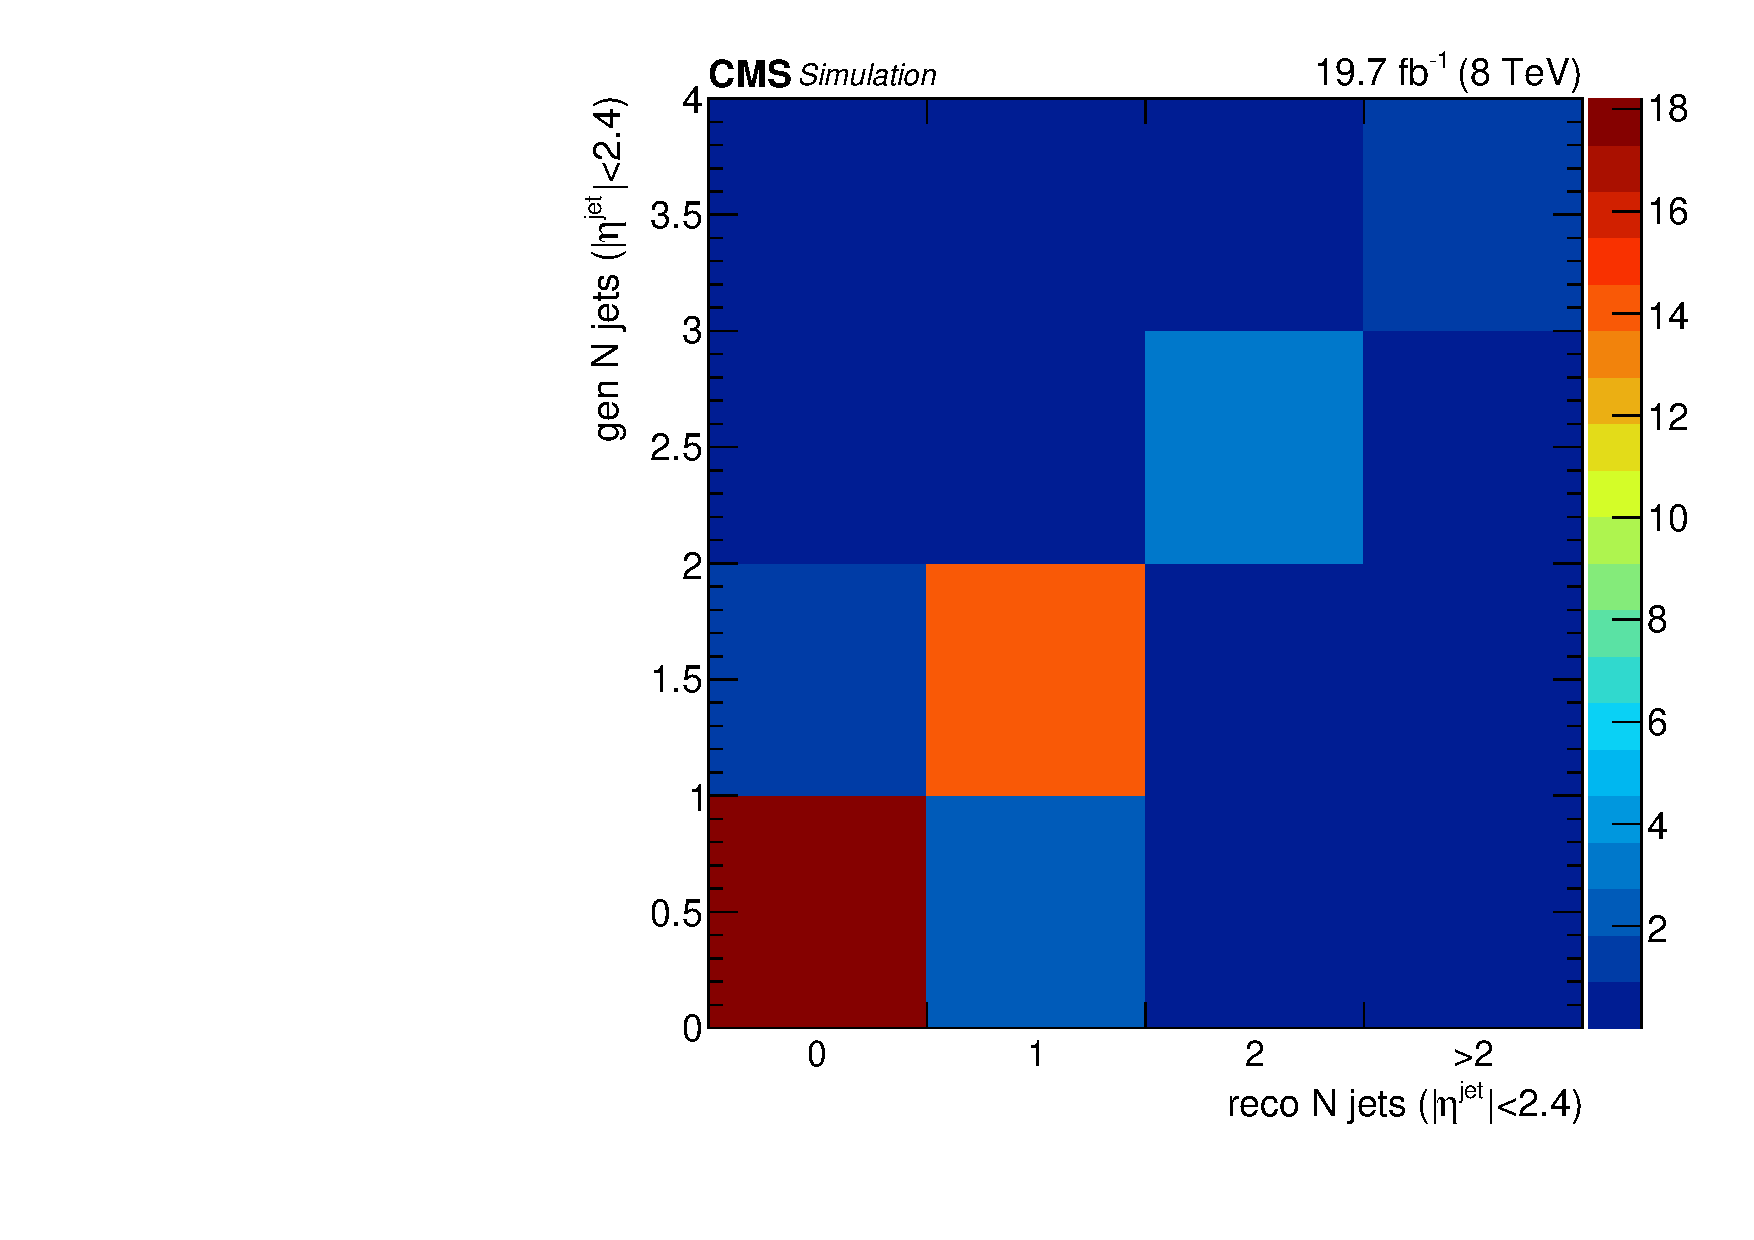
\includegraphics[width=\cmsFigWidth]{Figures/ResMat_qqggJJ_CentralJets_ZZTo4m_st_01_fr_Mad}
    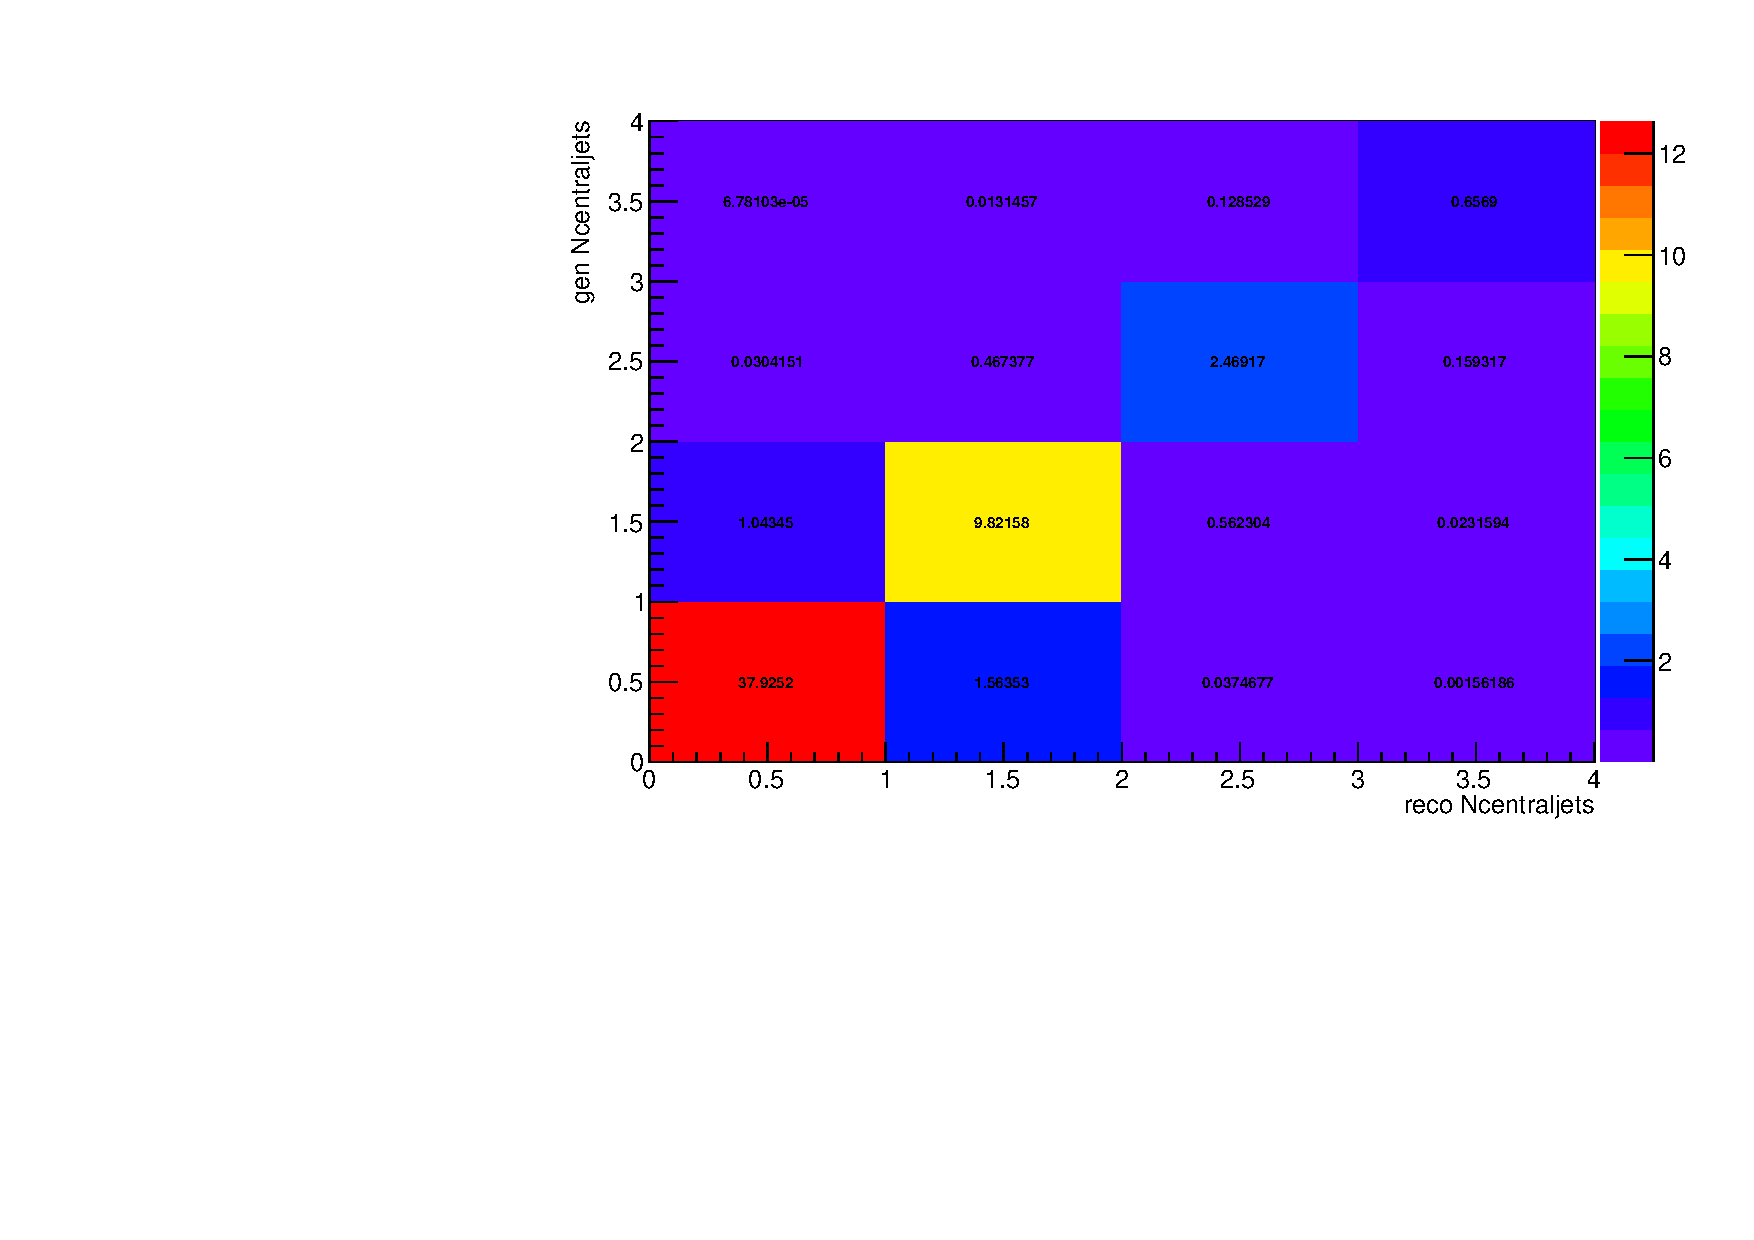
\includegraphics[width=\cmsFigWidth]{Figures/ResMat_qqggJJ_CentralJets_ZZTo4e_st_01_fr_Mad}
    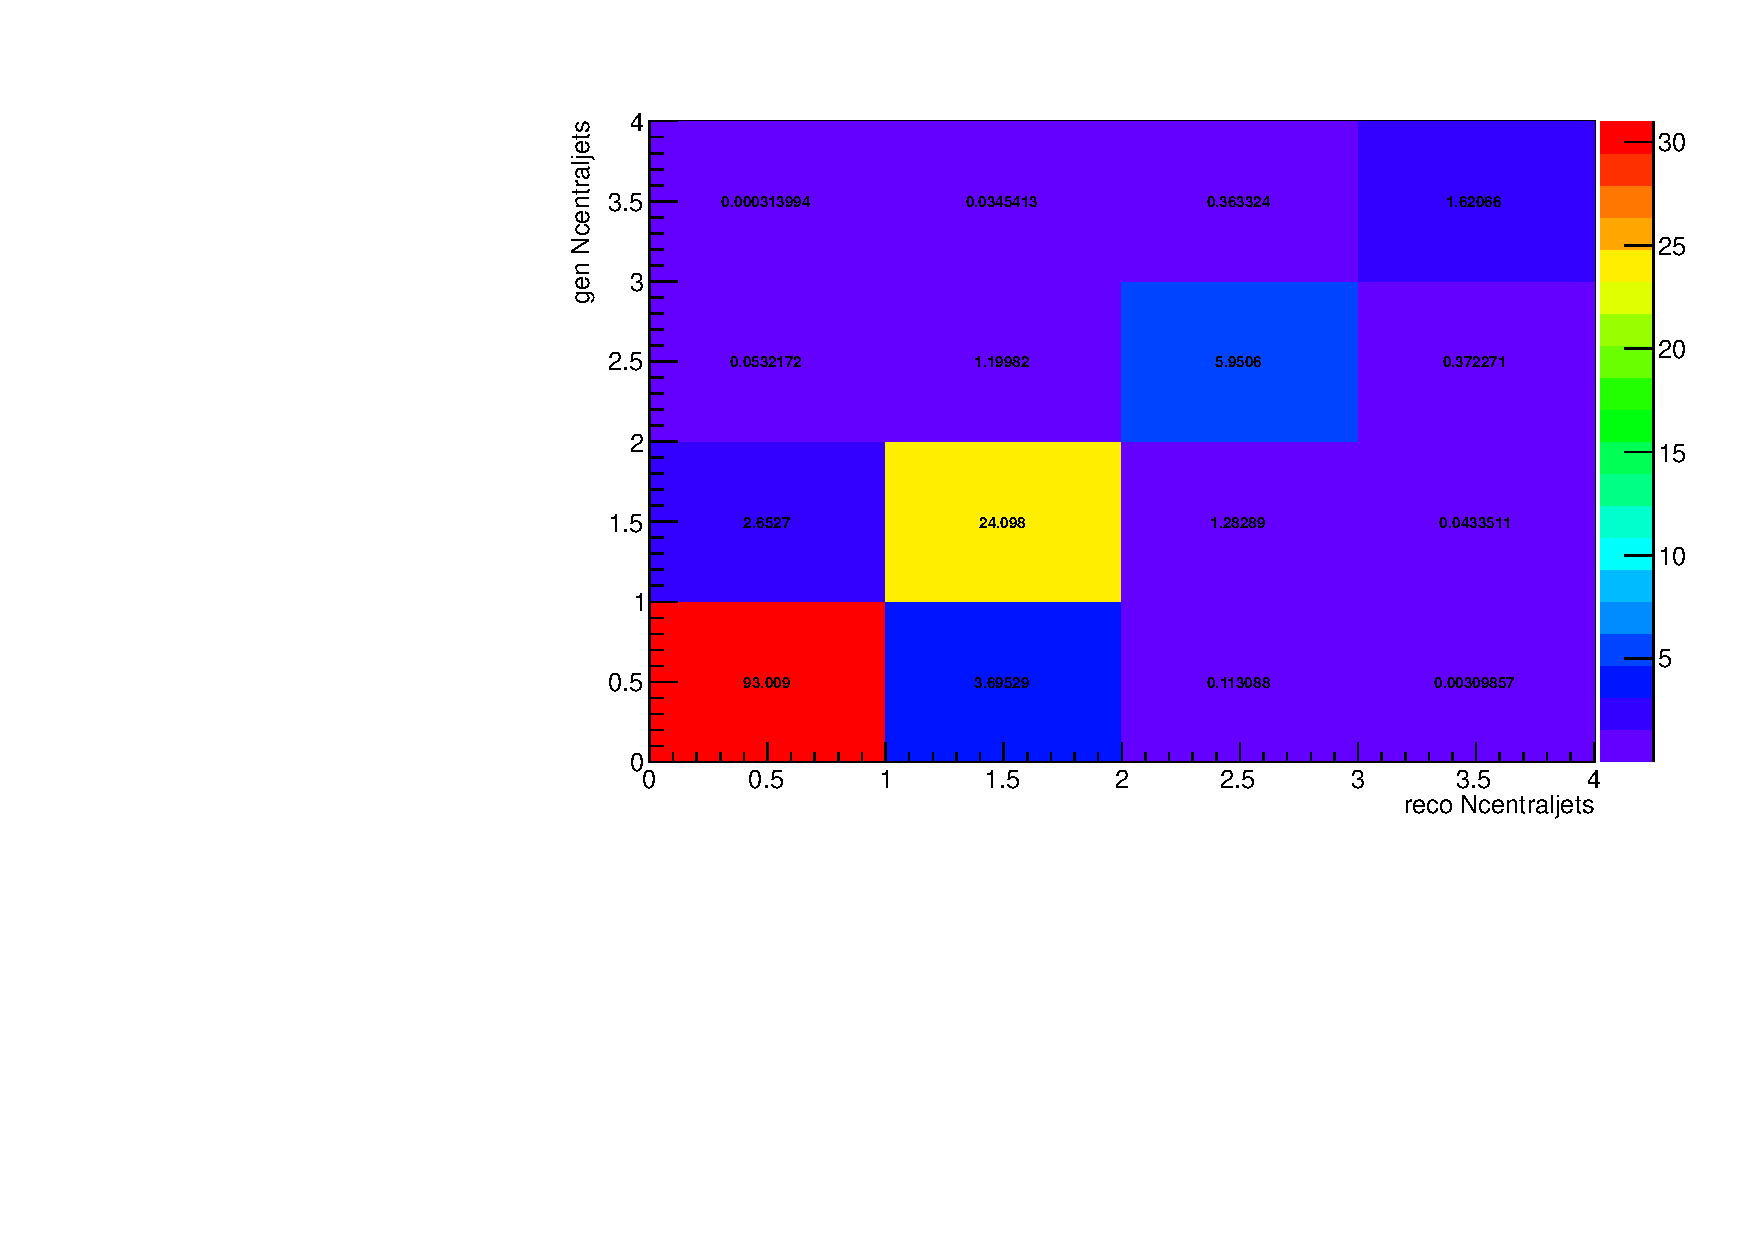
\includegraphics[width=\cmsFigWidth]{Figures/ResMat_qqggJJ_CentralJets_ZZTo2e2m_st_01_fr_Mad}     
 %   to generate (a) and (b) labels under the figures, you can use subfloat, but this is not recommended: takes too much space
 %   \subfloat[]{
\includegraphics[width=0.2\textwidth]{CMS-bw-logo}}\subfloat[]{
\includegraphics[width=0.2\textwidth]{CMScol}}
    \caption{Response matrices for the $N\ central\ jets$ distribution (with $\eta^{jet}<2.4$) , according to the final state:  $4\mu$ (top left), $4e$ (top right), $2e2\mu$  (bottom). Matrices are obtained using the  \texttt{MadGraph} set of samples. The tight fiducial region is considered.} 
    \label{fig:CentralJets_matrices}
  \end{center}
\end{figure}
\begin{figure}[hbtp]
  \begin{center}
    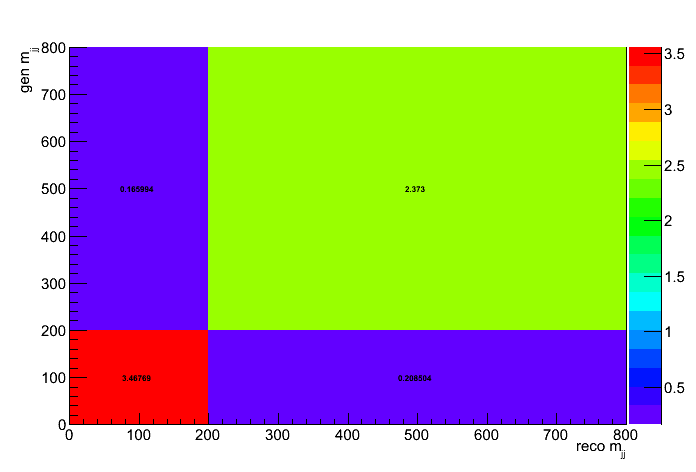
\includegraphics[width=\cmsFigWidth]{Figures/ResMat_qqggJJ_Mjj_ZZTo4m_st_01_fr_Mad}
    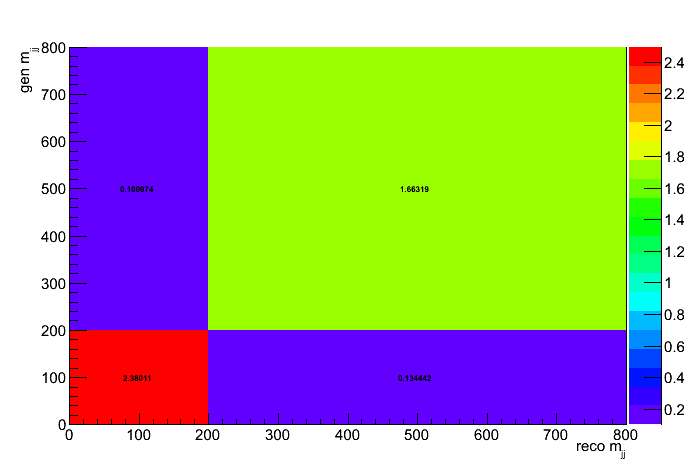
\includegraphics[width=\cmsFigWidth]{Figures/ResMat_qqggJJ_Mjj_ZZTo4e_st_01_fr_Mad}
    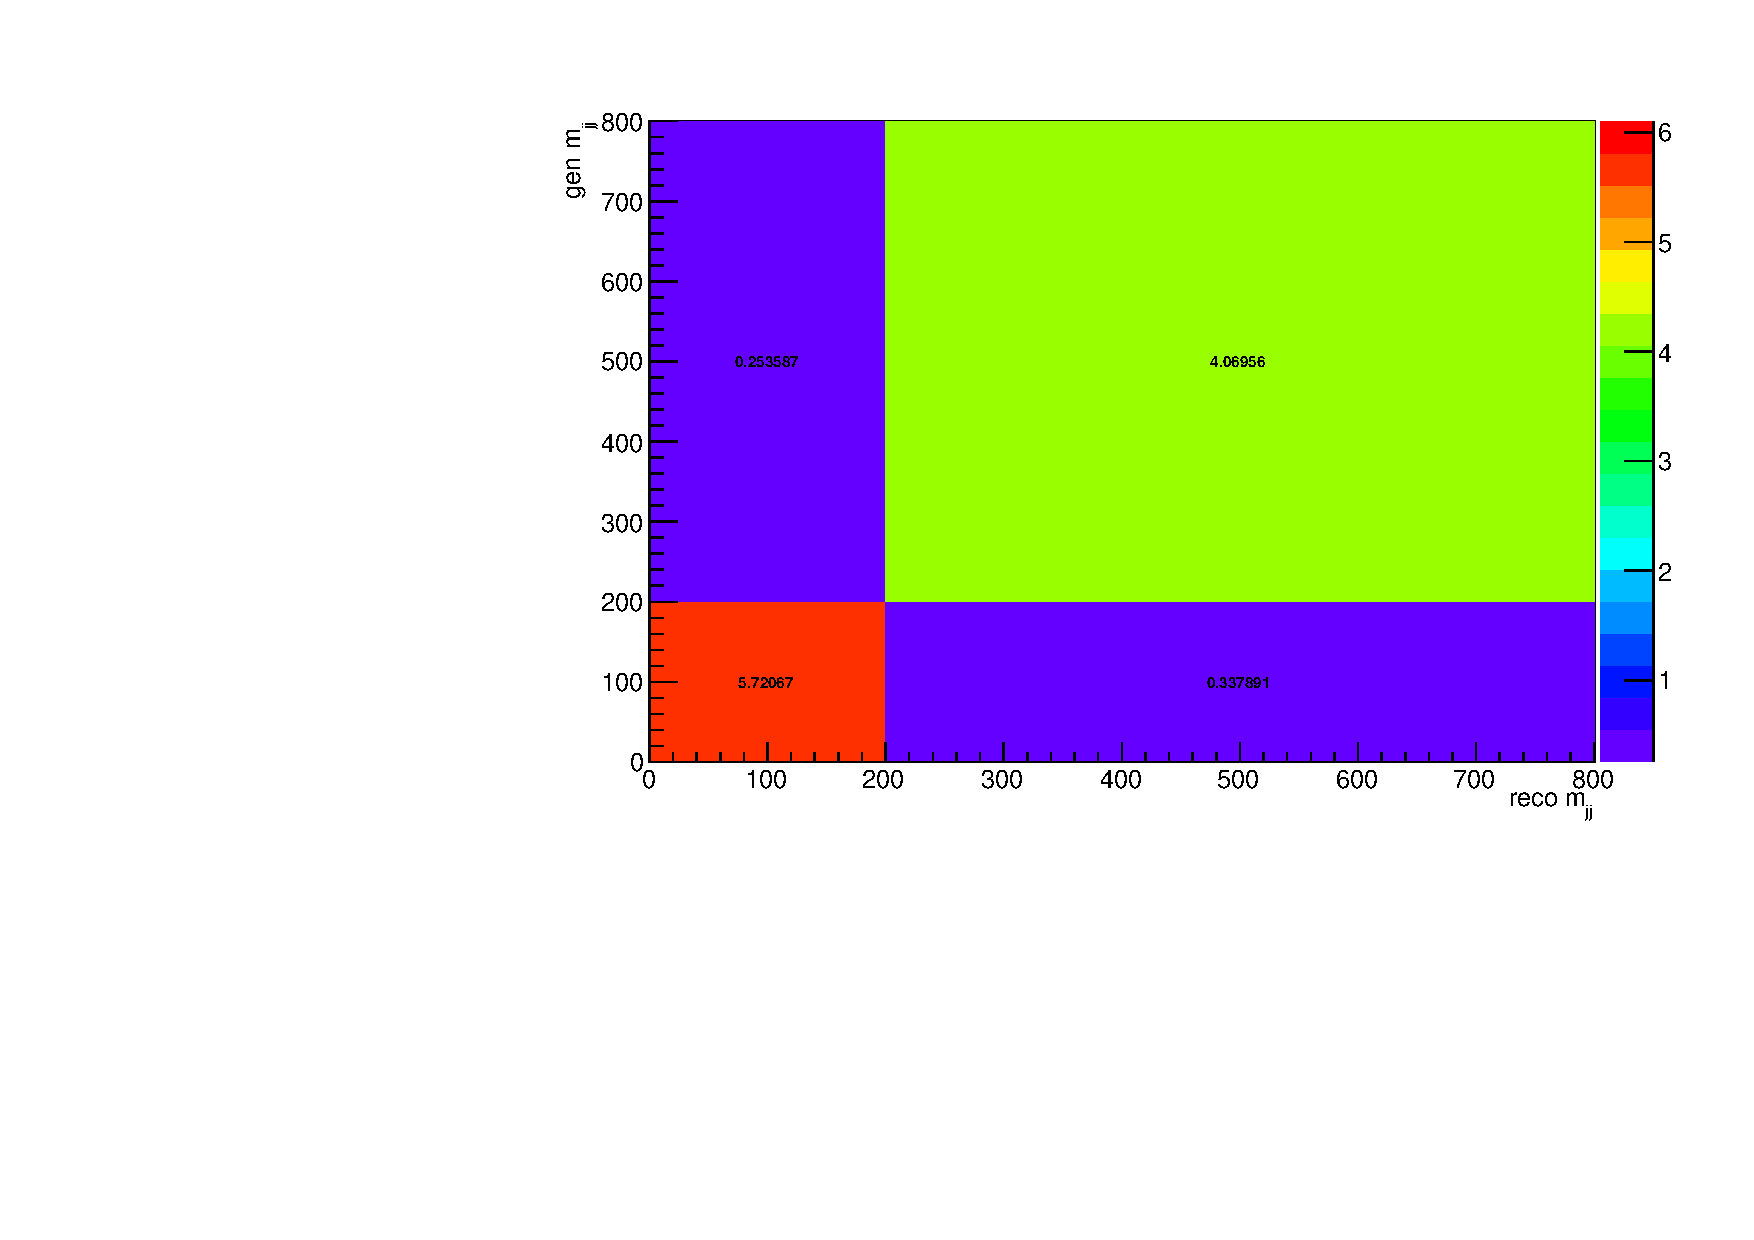
\includegraphics[width=\cmsFigWidth]{Figures/ResMat_qqggJJ_Mjj_ZZTo2e2m_st_01_fr_Mad}     
 %   to generate (a) and (b) labels under the figures, you can use subfloat, but this is not recommended: takes too much space
 %   \subfloat[]{
\includegraphics[width=0.2\textwidth]{CMS-bw-logo}}\subfloat[]{\includegraphics[width=0.2\textwidth]{CMScol}}
    \caption{Response matrices for the $m_{jj}$ distribution, according to the final state:  $4\mu$ (top left), $4e$ (top right), $2e2\mu$  (bottom). Matrices are obtained using the  \texttt{MadGraph} set of samples. The tight fiducial region is considered.} 
    \label{fig:Mjj_matrices}
  \end{center}
\end{figure}
\begin{figure}[hbtp]
  \begin{center}
    \includegraphics[width=\cmsFigWidth]{Figures/ResMat_qqggJJ_CentralMjj_ZZTo4m_st_01_fr_Mad}
    \includegraphics[width=\cmsFigWidth]{Figures/ResMat_qqggJJ_CentralMjj_ZZTo4e_st_01_fr_Mad}
    \includegraphics[width=\cmsFigWidth]{Figures/ResMat_qqggJJ_CentralMjj_ZZTo2e2m_st_01_fr_Mad}     
 %   to generate (a) and (b) labels under the figures, you can use subfloat, but this is not recommended: takes too much space
 %   \subfloat[]{\includegraphics[width=0.2\textwidth]{CMS-bw-logo}}\subfloat[]{\includegraphics[width=0.2\textwidth]{CMScol}}
    \caption{Response matrices for the $m_{jj}$ distribution (with $\eta^{jet}<2.4$), according to the final state:  $4\mu$ (top left), $4e$ (top right), $2e2\mu$  (bottom). Matrices are obtained using the  \texttt{MadGraph} set of samples. The tight fiducial region is considered.} 
    \label{fig:CentralMjj_matrices}
  \end{center}
\end{figure}
\begin{figure}[hbtp]
  \begin{center}
    \includegraphics[width=\cmsFigWidth]{Figures/ResMat_qqggJJ_Deta_ZZTo4m_st_01_fr_Mad}
    \includegraphics[width=\cmsFigWidth]{Figures/ResMat_qqggJJ_Deta_ZZTo4e_st_01_fr_Mad}
    \includegraphics[width=\cmsFigWidth]{Figures/ResMat_qqggJJ_Deta_ZZTo2e2m_st_01_fr_Mad}     
 %   to generate (a) and (b) labels under the figures, you can use subfloat, but this is not recommended: takes too much space
 %   \subfloat[]{\includegraphics[width=0.2\textwidth]{CMS-bw-logo}}\subfloat[]{\includegraphics[width=0.2\textwidth]{CMScol}}
    \caption{Response matrices for the $\Delta\eta_{jj}$ distribution, according to the final state:  $4\mu$ (top left), $4e$ (top right), $2e2\mu$  (bottom). Matrices are obtained using the  \texttt{MadGraph} set of samples. The tight fiducial region is considered.} 
    \label{fig:Deta_matrices}
  \end{center}
\end{figure}
\begin{figure}[hbtp]
  \begin{center}
    \includegraphics[width=\cmsFigWidth]{Figures/ResMat_qqggJJ_CentralDeta_ZZTo4m_st_01_fr_Mad}
    \includegraphics[width=\cmsFigWidth]{Figures/ResMat_qqggJJ_CentralDeta_ZZTo4e_st_01_fr_Mad}
    \includegraphics[width=\cmsFigWidth]{Figures/ResMat_qqggJJ_CentralDeta_ZZTo2e2m_st_01_fr_Mad}     
 %   to generate (a) and (b) labels under the figures, you can use subfloat, but this is not recommended: takes too much space
 %   \subfloat[]{\includegraphics[width=0.2\textwidth]{CMS-bw-logo}}\subfloat[]{\includegraphics[width=0.2\textwidth]{CMScol}}
    \caption{Response matrices for the $\Delta\eta_{jj}$ distribution (with $\eta^{jet}<2.4$), according to the final state:  $4\mu$ (top left), $4e$ (top right), $2e2\mu$  (bottom). Matrices are obtained using the  \texttt{MadGraph} set of samples. The tight fiducial region is considered.} 
    \label{fig:CentralDeta_matrices}
  \end{center}
\end{figure}
\begin{figure}[hbtp]
  \begin{center}
    \includegraphics[width=\cmsFigWidth]{Figures/ResMat_qqggJJ_PtJet1_ZZTo4m_st_01_fr_Mad}
    \includegraphics[width=\cmsFigWidth]{Figures/ResMat_qqggJJ_PtJet1_ZZTo4e_st_01_fr_Mad}
    \includegraphics[width=\cmsFigWidth]{Figures/ResMat_qqggJJ_PtJet1_ZZTo2e2m_st_01_fr_Mad}     
 %   to generate (a) and (b) labels under the figures, you can use subfloat, but this is not recommended: takes too much space
 %   \subfloat[]{\includegraphics[width=0.2\textwidth]{CMS-bw-logo}}\subfloat[]{\includegraphics[width=0.2\textwidth]{CMScol}}
    \caption{Response matrices for the $p_{T}$ distribution of the leading jet, according to the final state:  $4\mu$ (top left), $4e$ (top right), $2e2\mu$  (bottom). Matrices are obtained using the  \texttt{MadGraph} set of samples. The tight fiducial region is considered. } 
    \label{fig:PtJet1_matrices}
  \end{center}
\end{figure}
\begin{figure}[hbtp]
  \begin{center}
    \includegraphics[width=\cmsFigWidth]{Figures/ResMat_qqggJJ_PtJet2_ZZTo4m_st_01_fr_Mad}
    \includegraphics[width=\cmsFigWidth]{Figures/ResMat_qqggJJ_PtJet2_ZZTo4e_st_01_fr_Mad}
    \includegraphics[width=\cmsFigWidth]{Figures/ResMat_qqggJJ_PtJet2_ZZTo2e2m_st_01_fr_Mad}     
 %   to generate (a) and (b) labels under the figures, you can use subfloat, but this is not recommended: takes too much space
 %   \subfloat[]{\includegraphics[width=0.2\textwidth]{CMS-bw-logo}}\subfloat[]{\includegraphics[width=0.2\textwidth]{CMScol}}
    \caption{Response matrices for the $p_{T}$ distribution of the sub-leading jet, according to the final state:  $4\mu$ (top left), $4e$ (top right), $2e2\mu$  (bottom). Matrices are obtained using the  \texttt{MadGraph} set of samples. The tight fiducial region is considered.} 
    \label{fig:PtJet2_matrices}
  \end{center}
\end{figure}

\begin{figure}[hbtp]
  \begin{center}
    \includegraphics[width=\cmsFigWidth]{Figures/ResMat_qqggJJ_EtaJet1_ZZTo4m_st_01_fr_Mad}
    \includegraphics[width=\cmsFigWidth]{Figures/ResMat_qqggJJ_EtaJet1_ZZTo4e_st_01_fr_Mad}
    \includegraphics[width=\cmsFigWidth]{Figures/ResMat_qqggJJ_EtaJet1_ZZTo2e2m_st_01_fr_Mad}     
 %   to generate (a) and (b) labels under the figures, you can use subfloat, but this is not recommended: takes too much space
 %   \subfloat[]{\includegraphics[width=0.2\textwidth]{CMS-bw-logo}}\subfloat[]{\includegraphics[width=0.2\textwidth]{CMScol}}
    \caption{Response matrices for the $\eta$ distribution of the leading jet, according to the final state:  $4\mu$ (top left), $4e$ (top right), $2e2\mu$  (bottom). Matrices are obtained using the  \texttt{MadGraph} set of samples. The tight fiducial region is considered.} 
    \label{fig:EtaJet1_matrices}
  \end{center}
\end{figure}
\begin{figure}[hbtp]
  \begin{center}
    \includegraphics[width=\cmsFigWidth]{Figures/ResMat_qqggJJ_EtaJet2_ZZTo4m_st_01_fr_Mad}
    \includegraphics[width=\cmsFigWidth]{Figures/ResMat_qqggJJ_EtaJet2_ZZTo4e_st_01_fr_Mad}
    \includegraphics[width=\cmsFigWidth]{Figures/ResMat_qqggJJ_EtaJet2_ZZTo2e2m_st_01_fr_Mad}     
 %   to generate (a) and (b) labels under the figures, you can use subfloat, but this is not recommended: takes too much space
 %   \subfloat[]{\includegraphics[width=0.2\textwidth]{CMS-bw-logo}}\subfloat[]{\includegraphics[width=0.2\textwidth]{CMScol}}
    \caption{Response matrices for the $\eta$ distribution of the sub-leading jet, according to the final state:  $4\mu$ (top left), $4e$ (top right), $2e2\mu$  (bottom). Matrices are obtained using the  \texttt{MadGraph} set of samples. The tight fiducial region is considered.} 
    \label{fig:EtaJet2_matrices}
  \end{center}
\end{figure}
\clearpage

\begin{figure}[hbtp]
  \begin{center}
    \includegraphics[width=\cmsFigWidth]{Figures/Mass_ZZTo4m_Pow_fr_binwidth}
    \includegraphics[width=\cmsFigWidth]{Figures/Mass_ZZTo4e_Pow_fr_binwidth}
    \includegraphics[width=\cmsFigWidth]{Figures/Mass_ZZTo2e2m_Pow_fr_binwidth}  
    \includegraphics[width=\cmsFigWidth]{Figures/Mass_ZZTo4l_Pow_fr}    
 %   to generate (a) and (b) labels under the figures, you can use subfloat, but this is not recommended: takes too much space
 %   \subfloat[]{\includegraphics[width=0.2\textwidth]{CMS-bw-logo}}\subfloat[]{\includegraphics[width=0.2\textwidth]{CMScol}}
    \caption{\footnotesize{Data (red), unfolded data (blue), generated (dashed blue) and MC reconstructed (dashed red) $m_{ZZ}$ distributions, according to the final state: 
$4\mu$ (top left), $4e$ (top right), $2e2\mu$  (bottom left),  $4\ell$ (bottom right). The unfolded distributions are obtained  in the tight fiducial region using the SVD algorithm, with $k_{reg} = 4$, and compared to predictions from the \texttt{Powheg} set of samples.}} 
    \label{fig:Mass_unfolding}
  \end{center}
\end{figure}

\begin{figure}[hbtp]
  \begin{center}
    \includegraphics[width=\cmsFigWidth]{Figures/Jets_ZZTo4m_Mad_fr_binwidth}
    \includegraphics[width=\cmsFigWidth]{Figures/Jets_ZZTo4e_Mad_fr_binwidth}
    \includegraphics[width=\cmsFigWidth]{Figures/Jets_ZZTo2e2m_Mad_fr_binwidth}     
    \includegraphics[width=\cmsFigWidth]{Figures/Jets_ZZTo4l_Mad_fr}    
 %   to generate (a) and (b) labels under the figures, you can use subfloat, but this is not recommended: takes too much space
 %   \subfloat[]{\includegraphics[width=0.2\textwidth]{CMS-bw-logo}}\subfloat[]{\includegraphics[width=0.2\textwidth]{CMScol}}
    \caption{\footnotesize{Data (red), unfolded data (blue), generated (dashed blue) and MC reconstructed (dashed red) $N\ jets$ distributions, according to the final state: (top left) $4\mu$, (top right) $4e$, (bottom left) $2e2\mu$, (bottom right) $4\ell$. The unfolded distributions are obtained in the tight fiducial region using the D'Agostini algorithm, with 4 iterations, and compared to predictions from the \texttt{MadGraph} set of samples.}} 
    \label{fig:Jets_unfolding}
  \end{center}
\end{figure}

\begin{figure}[hbtp]
  \begin{center}
    \includegraphics[width=\cmsFigWidth]{Figures/CentralJets_ZZTo4m_Mad_fr_binwidth}
    \includegraphics[width=\cmsFigWidth]{Figures/CentralJets_ZZTo4e_Mad_fr_binwidth}
    \includegraphics[width=\cmsFigWidth]{Figures/CentralJets_ZZTo2e2m_Mad_fr_binwidth}     
    \includegraphics[width=\cmsFigWidth]{Figures/CentralJets_ZZTo4l_Mad_fr}    
 %   to generate (a) and (b) labels under the figures, you can use subfloat, but this is not recommended: takes too much space
 %   \subfloat[]{\includegraphics[width=0.2\textwidth]{CMS-bw-logo}}\subfloat[]{\includegraphics[width=0.2\textwidth]{CMScol}}
    \caption{\footnotesize{Data (red), unfolded data (blue), generated (dashed blue) and MC reconstructed (dashed red) $N\ central\ jets$ distributions, according to the final state: (top left) $4\mu$, (top right) $4e$, (bottom left) $2e2\mu$, (bottom right) $4\ell$. The unfolded distributions are obtained in the tight fiducial region using the D'Agostini algorithm, with 4 iterations, and compared to predictions from the \texttt{MadGraph} set of samples.}} 
    \label{fig:CentralJets_unfolding}
  \end{center}
\end{figure}
%\clearpage
\begin{figure}[hbtp]
  \begin{center}
    \includegraphics[width=\cmsFigWidth]{Figures/Mjj_ZZTo4m_Mad_fr_binwidth}
    \includegraphics[width=\cmsFigWidth]{Figures/Mjj_ZZTo4e_Mad_fr_binwidth}
    \includegraphics[width=\cmsFigWidth]{Figures/Mjj_ZZTo2e2m_Mad_fr_binwidth}   
    \includegraphics[width=\cmsFigWidth]{Figures/Mjj_ZZTo4l_Mad_fr}      
 %   to generate (a) and (b) labels under the figures, you can use subfloat, but this is not recommended: takes too much space
 %   \subfloat[]{\includegraphics[width=0.2\textwidth]{CMS-bw-logo}}\subfloat[]{\includegraphics[width=0.2\textwidth]{CMScol}}
    \caption{\footnotesize{Data (red), unfolded data (blue), generated (dashed blue) and MC reconstructed (dashed red) $m_{jj}$ distributions, according to the final state: (top left) $4\mu$, (top right) $4e$, (bottom left) $2e2\mu$, (bottom right) $4\ell$. The unfolded distributions are obtained in the tight fiducial region using the D'Agostini algorithm, with 4 iterations, and compared to predictions from the \texttt{MadGraph} set of samples.}} 
    \label{fig:Mjj_unfolding}
  \end{center}
\end{figure}
\begin{figure}[hbtp]
  \begin{center}
    \includegraphics[width=\cmsFigWidth]{Figures/CentralMjj_ZZTo4m_Mad_fr_binwidth}
    \includegraphics[width=\cmsFigWidth]{Figures/CentralMjj_ZZTo4e_Mad_fr_binwidth}
    \includegraphics[width=\cmsFigWidth]{Figures/CentralMjj_ZZTo2e2m_Mad_fr_binwidth}   
    \includegraphics[width=\cmsFigWidth]{Figures/CentralMjj_ZZTo4l_Mad_fr}      
 %   to generate (a) and (b) labels under the figures, you can use subfloat, but this is not recommended: takes too much space
 %   \subfloat[]{\includegraphics[width=0.2\textwidth]{CMS-bw-logo}}\subfloat[]{\includegraphics[width=0.2\textwidth]{CMScol}}
    \caption{\footnotesize{Data (red), unfolded data (blue), generated (dashed blue) and MC reconstructed (dashed red) $m_{jj}$ distributions (using central jets with $\eta^{jet}<2.4$), according to the final state: (top left) $4\mu$, (top right) $4e$, (bottom left) $2e2\mu$, (bottom right) $4\ell$. The unfolded distributions are obtained in the tight fiducial region using the D'Agostini algorithm, with 4 iterations, and compared to predictions from the \texttt{MadGraph} set of samples.}} 
    \label{fig:CentralMjj_unfolding}
  \end{center}
\end{figure}

\begin{figure}[hbtp]
  \begin{center}
    \includegraphics[width=\cmsFigWidth]{Figures/Deta_ZZTo4m_Mad_fr_binwidth}
    \includegraphics[width=\cmsFigWidth]{Figures/Deta_ZZTo4e_Mad_fr_binwidth}
    \includegraphics[width=\cmsFigWidth]{Figures/Deta_ZZTo2e2m_Mad_fr_binwidth}  
    \includegraphics[width=\cmsFigWidth]{Figures/Deta_ZZTo4l_Mad_fr}       
 %   to generate (a) and (b) labels under the figures, you can use subfloat, but this is not recommended: takes too much space
 %   \subfloat[]{\includegraphics[width=0.2\textwidth]{CMS-bw-logo}}\subfloat[]{\includegraphics[width=0.2\textwidth]{CMScol}}
    \caption{\footnotesize{Data (red), unfolded data (blue), generated (dashed blue) and MC reconstructed (dashed red) $\Delta\eta_{jj}$ distributions, according to the final state: (top left) $4\mu$, (top right) $4e$, (bottom left) $2e2\mu$, (bottom right) $4\ell$. The unfolded distributions are obtained in the tight fiducial region using the D'Agostini algorithm, with 4 iterations, and compared to predictions from the \texttt{MadGraph} set of samples.}} 
    \label{fig:Deta_unfolding}
  \end{center}
\end{figure}
\begin{figure}[hbtp]
  \begin{center}
    \includegraphics[width=\cmsFigWidth]{Figures/CentralDeta_ZZTo4m_Mad_fr_binwidth}
    \includegraphics[width=\cmsFigWidth]{Figures/CentralDeta_ZZTo4e_Mad_fr_binwidth}
    \includegraphics[width=\cmsFigWidth]{Figures/CentralDeta_ZZTo2e2m_Mad_fr_binwidth}  
    \includegraphics[width=\cmsFigWidth]{Figures/CentralDeta_ZZTo4l_Mad_fr}       
 %   to generate (a) and (b) labels under the figures, you can use subfloat, but this is not recommended: takes too much space
 %   \subfloat[]{\includegraphics[width=0.2\textwidth]{CMS-bw-logo}}\subfloat[]{\includegraphics[width=0.2\textwidth]{CMScol}}
    \caption{\footnotesize{Data (red), unfolded data (blue), generated (dashed blue) and MC reconstructed (dashed red) $\Delta\eta_{jj}$ distributions (using central jets with $\eta^{jet}<2.4$), according to the final state: (top left) $4\mu$, (top right) $4e$, (bottom left) $2e2\mu$, (bottom right) $4\ell$. The unfolded distributions are obtained in the tight fiducial region using the D'Agostini algorithm, with 4 iterations, and compared to predictions from the \texttt{MadGraph} set of samples.}} 
    \label{fig:CentralDeta_unfolding}
  \end{center}
\end{figure}

\begin{figure}[hbtp]
  \begin{center}
    \includegraphics[width=\cmsFigWidth]{Figures/PtJet1_ZZTo4m_Mad_fr_binwidth}
    \includegraphics[width=\cmsFigWidth]{Figures/PtJet1_ZZTo4e_Mad_fr_binwidth}
    \includegraphics[width=\cmsFigWidth]{Figures/PtJet1_ZZTo2e2m_Mad_fr_binwidth}  
    \includegraphics[width=\cmsFigWidth]{Figures/PtJet1_ZZTo4l_Mad_fr}       
 %   to generate (a) and (b) labels under the figures, you can use subfloat, but this is not recommended: takes too much space
 %   \subfloat[]{\includegraphics[width=0.2\textwidth]{CMS-bw-logo}}\subfloat[]{\includegraphics[width=0.2\textwidth]{CMScol}}
    \caption{\footnotesize{Data (red), unfolded data (blue), generated (dashed blue) and MC reconstructed (dashed red) $p_{T}^{jet1}$ distributions, according to the final state: (top left) $4\mu$, (top right) $4e$, (bottom left) $2e2\mu$, (bottom right) $4\ell$. The unfolded distributions are obtained in the tight fiducial region using the D'Agostini algorithm, with 4 iterations, and compared to predictions from the \texttt{MadGraph} set of samples.}} 
    \label{fig:PtJet1_unfolding}
  \end{center}
\end{figure}

\begin{figure}[hbtp]
  \begin{center}
    \includegraphics[width=\cmsFigWidth]{Figures/PtJet2_ZZTo4m_Mad_fr_binwidth}
    \includegraphics[width=\cmsFigWidth]{Figures/PtJet2_ZZTo4e_Mad_fr_binwidth}
    \includegraphics[width=\cmsFigWidth]{Figures/PtJet2_ZZTo2e2m_Mad_fr_binwidth}  
    \includegraphics[width=\cmsFigWidth]{Figures/PtJet2_ZZTo4l_Mad_fr}       
 %   to generate (a) and (b) labels under the figures, you can use subfloat, but this is not recommended: takes too much space
 %   \subfloat[]{\includegraphics[width=0.2\textwidth]{CMS-bw-logo}}\subfloat[]{\includegraphics[width=0.2\textwidth]{CMScol}}
    \caption{\footnotesize{Data (red), unfolded data (blue), generated (dashed blue) and MC reconstructed (dashed red) $p_{T}^{jet2}$ distributions, according to the final state: (top left) $4\mu$, (top right) $4e$, (bottom left) $2e2\mu$, (bottom right) $4\ell$. The unfolded distributions are obtained in the tight fiducial region using the D'Agostini algorithm, with 4 iterations, and compared to predictions from the \texttt{MadGraph} set of samples.}} 
    \label{fig:PtJet2_unfolding}
  \end{center}
\end{figure}


\begin{figure}[hbtp]
  \begin{center}
    \includegraphics[width=\cmsFigWidth]{Figures/EtaJet1_ZZTo4m_Mad_fr_binwidth}
    \includegraphics[width=\cmsFigWidth]{Figures/EtaJet1_ZZTo4e_Mad_fr_binwidth}
    \includegraphics[width=\cmsFigWidth]{Figures/EtaJet1_ZZTo2e2m_Mad_fr_binwidth}  
    \includegraphics[width=\cmsFigWidth]{Figures/EtaJet1_ZZTo4l_Mad_fr}       
 %   to generate (a) and (b) labels under the figures, you can use subfloat, but this is not recommended: takes too much space
 %   \subfloat[]{\includegraphics[width=0.2\textwidth]{CMS-bw-logo}}\subfloat[]{\includegraphics[width=0.2\textwidth]{CMScol}}
    \caption{\footnotesize{Data (red), unfolded data (blue), generated (dashed blue) and MC reconstructed (dashed red) $\eta^{jet1}$ distributions, according to the final state: (top left) $4\mu$, (top right) $4e$, (bottom left) $2e2\mu$, (bottom right) $4\ell$. The unfolded distributions are obtained in the tight fiducial region using the D'Agostini algorithm, with 4 iterations, and compared to predictions from the \texttt{MadGraph} set of samples.}} 
    \label{fig:EtaJet1_unfolding}
  \end{center}
\end{figure}

\begin{figure}[hbtp]
  \begin{center}
    \includegraphics[width=\cmsFigWidth]{Figures/EtaJet2_ZZTo4m_Mad_fr_binwidth}
    \includegraphics[width=\cmsFigWidth]{Figures/EtaJet2_ZZTo4e_Mad_fr_binwidth}
    \includegraphics[width=\cmsFigWidth]{Figures/EtaJet2_ZZTo2e2m_Mad_fr_binwidth}  
    \includegraphics[width=\cmsFigWidth]{Figures/EtaJet2_ZZTo4l_Mad_fr}       
 %   to generate (a) and (b) labels under the figures, you can use subfloat, but this is not recommended: takes too much space
 %   \subfloat[]{\includegraphics[width=0.2\textwidth]{CMS-bw-logo}}\subfloat[]{\includegraphics[width=0.2\textwidth]{CMScol}}
    \caption{\footnotesize{Data (red), unfolded data (blue), generated (dashed blue) and MC reconstructed (dashed red) $\eta^{jet2}$ distributions, according to the final state: (top left) $4\mu$, (top right) $4e$, (bottom left) $2e2\mu$, (bottom right) $4\ell$. The unfolded distributions are obtained in the tight fiducial region using the D'Agostini algorithm, with 4 iterations, and compared to predictions from the \texttt{MadGraph} set of samples.}} 
    \label{fig:EtaJet2_unfolding}
  \end{center}
\end{figure}
\clearpage
\begin{figure}[hbtp]
  \begin{center}
    \includegraphics[width=\cmsFigWidth]{Figures/DiffCrossSecZZTo4mMass_Unfolded_fr_Powheg_norm.png}     
    \includegraphics[width=\cmsFigWidth]{Figures/DiffCrossSecZZTo4eMass_Unfolded_fr_Powheg_norm.png}     
    \includegraphics[width=\cmsFigWidth]{Figures/DiffCrossSecZZTo2e2mMass_Unfolded_fr_Powheg_norm.png}       
    \includegraphics[width=\cmsFigWidth]{Figures/DiffCrossSecZZTo4lMass_Unfolded_fr_Powheg_norm.png}       
 %   to generate (a) and (b) labels under the figures, you can use subfloat, but this is not recommended: takes too much space
 %   \subfloat[]{\includegraphics[width=0.2\textwidth]{CMS-bw-logo}}\subfloat[]{\includegraphics[width=0.2\textwidth]{CMScol}}%
    \caption{\footnotesize{Normalized differential cross-sections as a function of the  invariant mass of the 4 lepton system, according to the final state: $4\mu$ (top left), $4e$ (top right), $2e2\mu$  (bottom left),  $4\ell$ (bottom right). Cross-sections are extracted in the tight fiducial region and compared to predictions from the \texttt{Powheg}, \texttt{MadGraph} and \texttt{MadGraph5\_aMCatNLO} sets of samples.}}
    \label{fig:diff_xs_mass}
  \end{center}
\end{figure}

\begin{figure}[hbtp]
  \begin{center}
    \includegraphics[width=\cmsFigWidth]{Figures/DiffCrossSecZZTo4mJets_Unfolded_fr_MadGraph_norm.png}     
    \includegraphics[width=\cmsFigWidth]{Figures/DiffCrossSecZZTo4eJets_Unfolded_fr_MadGraph_norm.png}     
    \includegraphics[width=\cmsFigWidth]{Figures/DiffCrossSecZZTo2e2mJets_Unfolded_fr_MadGraph_norm.png}       
    \includegraphics[width=\cmsFigWidth]{Figures/DiffCrossSecZZTo4lJets_Unfolded_fr_MadGraph_norm.png}       
 %   to generate (a) and (b) labels under the figures, you can use subfloat, but this is not recommended: takes too much space
 %   \subfloat[]{\includegraphics[width=0.2\textwidth]{CMS-bw-logo}}\subfloat[]{\includegraphics[width=0.2\textwidth]{CMScol}}
    \caption{\footnotesize{Normalized differential cross-sections as a function of the number of jets in the event, according to the final state: $4\mu$ (top left), $4e$ (top right), $2e2\mu$  (bottom left),  $4\ell$ (bottom right). Cross-sections are extracted in the tight fiducial region and compared to predictions from the \texttt{MadGraph}, \texttt{Powheg} and \texttt{MadGraph5\_aMCatNLO} sets of samples.}}
    \label{fig:diff_xs_jets}
  \end{center}
\end{figure}

\begin{figure}[hbtp]
  \begin{center}
    \includegraphics[width=\cmsFigWidth]{Figures/DiffCrossSecZZTo4mCentralJets_Unfolded_fr_MadGraph_norm.png}     
    \includegraphics[width=\cmsFigWidth]{Figures/DiffCrossSecZZTo4eCentralJets_Unfolded_fr_MadGraph_norm.png}     
    \includegraphics[width=\cmsFigWidth]{Figures/DiffCrossSecZZTo2e2mCentralJets_Unfolded_fr_MadGraph_norm.png}       
    \includegraphics[width=\cmsFigWidth]{Figures/DiffCrossSecZZTo4lCentralJets_Unfolded_fr_MadGraph_norm.png}       
 %   to generate (a) and (b) labels under the figures, you can use subfloat, but this is not recommended: takes too much space
 %   \subfloat[]{\includegraphics[width=0.2\textwidth]{CMS-bw-logo}}\subfloat[]{\includegraphics[width=0.2\textwidth]{CMScol}}
    \caption{\footnotesize{Normalized differential cross-sections as a function of the number of central jets in the event, according to the final state: $4\mu$ (top left), $4e$ (top right), $2e2\mu$  (bottom left),  $4\ell$ (bottom right). Cross-sections are extracted in the tight fiducial region and compared to predictions from the \texttt{MadGraph}, \texttt{Powheg}  and \texttt{MadGraph5\_aMCatNLO} sets of samples.}}
    \label{fig:diff_xs_centraljets}
  \end{center}
\end{figure}

\begin{figure}[hbtp]
  \begin{center}
    \includegraphics[width=\cmsFigWidth]{Figures/DiffCrossSecZZTo4mMjj_Unfolded_fr_MadGraph_norm.png}     
    \includegraphics[width=\cmsFigWidth]{Figures/DiffCrossSecZZTo4eMjj_Unfolded_fr_MadGraph_norm.png}     
    \includegraphics[width=\cmsFigWidth]{Figures/DiffCrossSecZZTo2e2mMjj_Unfolded_fr_MadGraph_norm.png}       
    \includegraphics[width=\cmsFigWidth]{Figures/DiffCrossSecZZTo4lMjj_Unfolded_fr_MadGraph_norm.png}       
 %   to generate (a) and (b) labels under the figures, you can use subfloat, but this is not recommended: takes too much space
 %   \subfloat[]{\includegraphics[width=0.2\textwidth]{CMS-bw-logo}}\subfloat[]{\includegraphics[width=0.2\textwidth]{CMScol}}
    \caption{\footnotesize{Normalized differential cross-sections as a function of the invariant mass of the most energetic jets in the event, according to the final state: $4\mu$ (top left), $4e$ (top right), $2e2\mu$  (bottom left),  $4\ell$ (bottom right). Cross-sections are extracted in the tight fiducial region and compared to predictions from the \texttt{MadGraph}, \texttt{Powheg} and \texttt{MadGraph5\_aMCatNLO} sets of samples.}}
    \label{fig:diff_xs_mjj}
  \end{center}
\end{figure}

\begin{figure}[hbtp]
  \begin{center}
    \includegraphics[width=\cmsFigWidth]{Figures/DiffCrossSecZZTo4mCentralMjj_Unfolded_fr_MadGraph_norm.png}     
    \includegraphics[width=\cmsFigWidth]{Figures/DiffCrossSecZZTo4eCentralMjj_Unfolded_fr_MadGraph_norm.png}     
    \includegraphics[width=\cmsFigWidth]{Figures/DiffCrossSecZZTo2e2mCentralMjj_Unfolded_fr_MadGraph_norm.png}       
    \includegraphics[width=\cmsFigWidth]{Figures/DiffCrossSecZZTo4lCentralMjj_Unfolded_fr_MadGraph_norm.png}       
 %   to generate (a) and (b) labels under the figures, you can use subfloat, but this is not recommended: takes too much space
 %   \subfloat[]{\includegraphics[width=0.2\textwidth]{CMS-bw-logo}}\subfloat[]{\includegraphics[width=0.2\textwidth]{CMScol}}
    \caption{\footnotesize{Normalized differential cross-sections as a function of the invariant mass of the most energetic central jets in the event, according to the final state: $4\mu$ (top left), $4e$ (top right), $2e2\mu$  (bottom left),  $4\ell$ (bottom right). Cross-sections are extracted in the tight fiducial region and compared to predictions from the \texttt{MadGraph}, \texttt{Powheg} and \texttt{MadGraph5\_aMCatNLO} sets of samples.}}
    \label{fig:diff_xs_centralmjj}
  \end{center}
\end{figure}

\begin{figure}[hbtp]
  \begin{center}
    \includegraphics[width=\cmsFigWidth]{Figures/DiffCrossSecZZTo4mDeta_Unfolded_fr_MadGraph_norm.png}     
    \includegraphics[width=\cmsFigWidth]{Figures/DiffCrossSecZZTo4eDeta_Unfolded_fr_MadGraph_norm.png}     
    \includegraphics[width=\cmsFigWidth]{Figures/DiffCrossSecZZTo2e2mDeta_Unfolded_fr_MadGraph_norm.png} 
    \includegraphics[width=\cmsFigWidth]{Figures/DiffCrossSecZZTo4lDeta_Unfolded_fr_MadGraph_norm.png}       
 %   to generate (a) and (b) labels under the figures, you can use subfloat, but this is not recommended: takes too much space
 %   \subfloat[]{\includegraphics[width=0.2\textwidth]{CMS-bw-logo}}\subfloat[]{\includegraphics[width=0.2\textwidth]{CMScol}}
    \caption{\footnotesize{Normalized differential cross-sections as a function of the pseudorapidity interval between the most energetic jets in the event, according to the final state: $4\mu$ (top left), $4e$ (top right), $2e2\mu$  (bottom left),  $4\ell$ (bottom right). Cross-sections are extracted in the tight fiducial region and compared to predictions from the \texttt{MadGraph}, \texttt{Powheg}  and \texttt{MadGraph5\_aMCatNLO} sets of samples.}}
    \label{fig:diff_xs_deta}
  \end{center}
\end{figure}

\begin{figure}[hbtp]
  \begin{center}
    \includegraphics[width=\cmsFigWidth]{Figures/DiffCrossSecZZTo4mCentralDeta_Unfolded_fr_MadGraph_norm.png}     
    \includegraphics[width=\cmsFigWidth]{Figures/DiffCrossSecZZTo4eCentralDeta_Unfolded_fr_MadGraph_norm.png}     
    \includegraphics[width=\cmsFigWidth]{Figures/DiffCrossSecZZTo2e2mCentralDeta_Unfolded_fr_MadGraph_norm.png}       
    \includegraphics[width=\cmsFigWidth]{Figures/DiffCrossSecZZTo4lCentralDeta_Unfolded_fr_MadGraph_norm.png}       
 %   to generate (a) and (b) labels under the figures, you can use subfloat, but this is not recommended: takes too much space
 %   \subfloat[]{\includegraphics[width=0.2\textwidth]{CMS-bw-logo}}\subfloat[]{\includegraphics[width=0.2\textwidth]{CMScol}}
    \caption{\footnotesize{Normalized differential cross-sections as a function of the pseudorapidity interval between the most energetic central jets in the event, according to the final state: $4\mu$ (top left), $4e$ (top right), $2e2\mu$  (bottom left),  $4\ell$ (bottom right). Cross-sections are extracted in the tight fiducial region and compared to predictions from the \texttt{MadGraph}, \texttt{Powheg}  and \texttt{MadGraph5\_aMCatNLO} sets of samples.}}
    \label{fig:diff_xs_centraldeta}
  \end{center}
\end{figure}

\begin{figure}[hbtp]
  \begin{center}
    \includegraphics[width=\cmsFigWidth]{Figures/DiffCrossSecZZTo4mPtJet1_Unfolded_fr_MadGraph_norm.png}     
    \includegraphics[width=\cmsFigWidth]{Figures/DiffCrossSecZZTo4ePtJet1_Unfolded_fr_MadGraph_norm.png}     
    \includegraphics[width=\cmsFigWidth]{Figures/DiffCrossSecZZTo2e2mPtJet1_Unfolded_fr_MadGraph_norm.png}       
    \includegraphics[width=\cmsFigWidth]{Figures/DiffCrossSecZZTo4lPtJet1_Unfolded_fr_MadGraph_norm.png}       
 %   to generate (a) and (b) labels under the figures, you can use subfloat, but this is not recommended: takes too much space
 %   \subfloat[]{\includegraphics[width=0.2\textwidth]{CMS-bw-logo}}\subfloat[]{\includegraphics[width=0.2\textwidth]{CMScol}}
    \caption{\footnotesize{Normalized differential cross-sections as a function of the leading jet transverse momentum in the event, according to the final state: $4\mu$ (top left), $4e$ (top right), $2e2\mu$  (bottom left),  $4\ell$ (bottom right). Cross-sections are extracted in the tight fiducial region and compared to predictions from the \texttt{MadGraph} and \texttt{Powheg} sets of samples.}}
    \label{fig:diff_xs_ptjet1}
  \end{center}
\end{figure}

\begin{figure}[hbtp]
  \begin{center}
    \includegraphics[width=\cmsFigWidth]{Figures/DiffCrossSecZZTo4mPtJet2_Unfolded_fr_MadGraph_norm.png}     
    \includegraphics[width=\cmsFigWidth]{Figures/DiffCrossSecZZTo4ePtJet2_Unfolded_fr_MadGraph_norm.png}     
    \includegraphics[width=\cmsFigWidth]{Figures/DiffCrossSecZZTo2e2mPtJet2_Unfolded_fr_MadGraph_norm.png}       
    \includegraphics[width=\cmsFigWidth]{Figures/DiffCrossSecZZTo4lPtJet2_Unfolded_fr_MadGraph_norm.png}       
 %   to generate (a) and (b) labels under the figures, you can use subfloat, but this is not recommended: takes too much space
 %   \subfloat[]{\includegraphics[width=0.2\textwidth]{CMS-bw-logo}}\subfloat[]{\includegraphics[width=0.2\textwidth]{CMScol}}
    \caption{\footnotesize{Normalized differential cross-sections as a function of the sub-leading jet transverse momentum in the event, according to the final state: $4\mu$ (top left), $4e$ (top right), $2e2\mu$  (bottom left),  $4\ell$ (bottom right). Cross-sections are extracted in the tight fiducial region and compared to predictions from the \texttt{MadGraph}, \texttt{Powheg}  and \texttt{MadGraph5\_aMCatNLO} sets of samples.}}
    \label{fig:diff_xs_ptjet2}
  \end{center}
\end{figure}
\begin{figure}[hbtp]
  \begin{center}
    \includegraphics[width=\cmsFigWidth]{Figures/DiffCrossSecZZTo4mEtaJet1_Unfolded_fr_MadGraph_norm.png}     
    \includegraphics[width=\cmsFigWidth]{Figures/DiffCrossSecZZTo4eEtaJet1_Unfolded_fr_MadGraph_norm.png}     
    \includegraphics[width=\cmsFigWidth]{Figures/DiffCrossSecZZTo2e2mEtaJet1_Unfolded_fr_MadGraph_norm.png}       
    \includegraphics[width=\cmsFigWidth]{Figures/DiffCrossSecZZTo4lEtaJet1_Unfolded_fr_MadGraph_norm.png}       
 %   to generate (a) and (b) labels under the figures, you can use subfloat, but this is not recommended: takes too much space
 %   \subfloat[]{\includegraphics[width=0.2\textwidth]{CMS-bw-logo}}\subfloat[]{\includegraphics[width=0.2\textwidth]{CMScol}}
    \caption{\footnotesize{Normalized differential cross-sections as a function of the leading jet pseudorapidity in the event, according to the final state: $4\mu$ (top left), $4e$ (top right), $2e2\mu$  (bottom left),  $4\ell$ (bottom right). Cross-sections are extracted in the tight fiducial region and compared to predictions from the \texttt{MadGraph}, \texttt{Powheg}  and \texttt{MadGraph5\_aMCatNLO} sets of samples.}}
    \label{fig:diff_xs_etajet1}
  \end{center}
\end{figure}

\begin{figure}[hbtp]
  \begin{center}
    \includegraphics[width=\cmsFigWidth]{Figures/DiffCrossSecZZTo4mEtaJet2_Unfolded_fr_MadGraph_norm.png}     
    \includegraphics[width=\cmsFigWidth]{Figures/DiffCrossSecZZTo4eEtaJet2_Unfolded_fr_MadGraph_norm.png}     
    \includegraphics[width=\cmsFigWidth]{Figures/DiffCrossSecZZTo2e2mEtaJet2_Unfolded_fr_MadGraph_norm.png}       
    \includegraphics[width=\cmsFigWidth]{Figures/DiffCrossSecZZTo4lEtaJet2_Unfolded_fr_MadGraph_norm.png}       
 %   to generate (a) and (b) labels under the figures, you can use subfloat, but this is not recommended: takes too much space
 %   \subfloat[]{\includegraphics[width=0.2\textwidth]{CMS-bw-logo}}\subfloat[]{\includegraphics[width=0.2\textwidth]{CMScol}}
    \caption{\footnotesize{Normalized differential cross-sections as a function of the sub-leading jet pseudorapidity in the event, according to the final state: $4\mu$ (top left), $4e$ (top right), $2e2\mu$  (bottom left),  $4\ell$ (bottom right). Cross-sections are extracted in the tight fiducial region and compared to predictions from the \texttt{MadGraph}, \texttt{Powheg}  and \texttt{MadGraph5\_aMCatNLO} sets of samples.}}  
    \label{fig:diff_xs_etajet2}
  \end{center}
\end{figure}
The systematic uncertainties in each bin are assessed from the variations of the nominal cross-section, by repeating the full analysis for every systematic variation. The difference with respect to the nominal value is taken as the systematic uncertainty for each bin and each measured observable. By using this method~\cite{SMP-14-016}, the possible correlations of the systematic uncertainties between bins are taken into account. Due to the normalization, those systematic uncertainties that are correlated across all bins of the measurement, and therefore mainly affect the normalization, cancel out at least partly. The errors also include the statistical error propagation through the unfolding method using the covariance matrix and the difference in the response matrix from \texttt{MadGraph} and \texttt{Powheg}.

For the $m_{ZZ}$ observable, the unfolded distributions are obtained with the SVD algorithm and the regularization
parameter $k_{reg}$ is chosen equal to 4. On the other hand, the other distributions are unfolded using the D'Agostini method, with 4 iterations. The unfolded distributions are presented from Figure~\ref{fig:Mass_unfolding} to Figure~\ref{fig:EtaJet2_unfolding}. The measurement is compared to the predictions from the \texttt{MadGraph} and \texttt{Powheg} sets of samples. The differential distributions normalized to the unity obtained in the tight fiducial region are presented 
%in Figures~\ref{fig:diff_xs_mass},~\ref{fig:diff_xs_jets},~\ref{fig:diff_xs_centraljets},~\ref{fig:diff_xs_mjj},~\ref{fig:diff_xs_centralmjj} and~\ref{fig:diff_xs_deta} 
from Figure~\ref{fig:diff_xs_mass} to Figure~\ref{fig:diff_xs_etajet2} for the $4\mu$, $4e$ and $2e2\mu$ decay channels 
and for their combination. The ratios between the measured distribution and the expected one from both the \texttt{MadGraph} and \texttt{Powheg} sets of samples are reported below each plot. Measurements are also compared with a set of samples in which \texttt{MadGraph5\_aMCatNLO} is used to generate $q\bar{q}\to ZZ$ signal processes. The  \texttt{Powheg} and \texttt{MadGraph5\_aMCatNLO} theoretical uncertainties due to the scale choice are estimated varying independently $\mu_R$ and $\mu_F$ by a factor from 0.5 to 2.\\ 
The total ZZ production cross-section as measured in each decay channel and for the combination of all channels in the wide and thight fiducial regions classified with respect to the number of jets and central jets is reported in Tables~\ref{tab:xs_njets},~\ref{tab:xs_ncentraljets},~\ref{tab:xs_njets_fr} and~\ref{tab:xs_ncentraljets_fr}.

\begin{table*}[htbH]
\begin{center}
\caption{\footnotesize{The total $ZZ$ production cross-section as measured in each decay channel and for the combination of all channels in the fiducial region $60< m_{Z_{1}}, m_{Z_{2}} < 120~\mathrm{GeV}$ classified with respect to the number of jets.}}
\label{tab:xs_njets}
%\scalebox{1.5\columnwidth}{!}{
%\doublespacing{
\begin{tabular}{lcc}
\hline Process & Number of jets ($|\eta^{jet}|<4.7$) &  Total cross-section [pb]\\
\hline $pp\to ZZ(4\mu) $ & $ 0 $ & $6.27\pm 0.82~\mathrm{(stat.)}\pm 0.39~\mathrm{(syst.)}$\\
$pp\to ZZ(4e) $ & $  0 $ & $5.84\pm 0.96~\mathrm{(stat.)}\pm 0.48~\mathrm{(syst.)}$\\
$pp\to ZZ(2e2\mu)$ & $ 0 $ &  $7.03\pm 0.67~\mathrm{(stat.)}\pm 0.56~\mathrm{(syst.)}$\\
\hline
\textbf{$pp\to ZZ(4\ell)$} & $0$ & $6.48 \pm 0.46~\mathrm{(stat.)}\pm 0.40~\mathrm{(syst.)}$ \\
\hline
$pp\to ZZ(4\mu) $ & $1$ & $1.03\pm 0.38~\mathrm{(stat.)}\pm 0.14~\mathrm{(syst.)}$\\
$pp\to ZZ(4e) $ &  $1$ & $1.02\pm 0.47~\mathrm{(stat.)}\pm 0.16~\mathrm{(syst.)}$\\
$pp\to ZZ(2e2\mu)$ & $1$ & $1.25\pm 0.32~\mathrm{(stat.)}\pm 0.26~\mathrm{(syst.)}$\\
\hline
\textbf{$pp\to ZZ(4\ell)$} & $1$ & $1.11 \pm 0.22~\mathrm{(stat.)}\pm 0.10~\mathrm{(syst.)}$ \\
\hline 
$pp\to ZZ(4\mu) $ & $2$ & $0.08\pm 0.11~\mathrm{(stat.)}\pm 0.06~\mathrm{(syst.)}$\\
$pp\to ZZ(4e) $ &  $2$ & $0.60\pm 0.33~\mathrm{(stat.)}\pm 0.07~\mathrm{(syst.)}$\\
$pp\to ZZ(2e2\mu)$ & $2$ & $0.16\pm 0.13~\mathrm{(stat.)}\pm 0.08~\mathrm{(syst.)}$\\
\hline
\textbf{$pp\to ZZ(4\ell)$} & $2$ & $0.15 \pm 0.08~\mathrm{(stat.)}\pm 0.03~\mathrm{(syst.)}$ \\
\hline 
$pp\to ZZ(4\mu) $ & $>2$ & $0.18\pm 0.14~\mathrm{(stat.)}\pm 0.06~\mathrm{(syst.)}$\\
$pp\to ZZ(4e) $ & $>2$ & $(0.32\pm 0.19~\mathrm{(stat.)}\pm 0.43~\mathrm{(syst.)}) \cdot 10^{-3}$\\
$pp\to ZZ(2e2\mu)$ & $>2$ & $(0.89 \pm 0.81~\mathrm{(stat.)}\pm 1.23~\mathrm{(syst.)})\cdot 10^{-4}$\\
\hline
\textbf{$pp\to ZZ(4\ell)$} & $>2$ & $(1.1\pm 0.7~\mathrm{(stat.)} \pm 1.2~\mathrm{(syst.)}) \cdot 10^{-4}$ \\
\hline \\
\end{tabular}%}
\end{center}
\end{table*}
\begin{table*}[htbH]
\begin{center}
\caption{\footnotesize{The total $ZZ$ production cross-section as measured in each decay channel and for the combination of all channels in the fiducial region $60< m_{Z_{1}}, m_{Z_{2}} < 120~\mathrm{GeV}$ classified with respect to the number of central jets.}}
\label{tab:xs_ncentraljets}
%\scalebox{1.5\columnwidth}{!}{
%\doublespacing{
\begin{tabular}{lcc}
\hline Process & Number of jets ($|\eta^{jet}|< 2.4$) & Total cross-section [pb]\\
\hline $pp\to ZZ(4\mu) $ & $ 0 $ & $6.27\pm 0.82~\mathrm{(stat.)}\pm 0.42~\mathrm{(syst.)}$\\
$pp\to ZZ(4e) $ & $  0 $ & $6.05\pm 0.97~\mathrm{(stat.)}\pm 0.52~\mathrm{(syst.)}$\\
$pp\to ZZ(2e2\mu)$ & $ 0 $ &  $7.15\pm 0.67~\mathrm{(stat.)}\pm 0.58~\mathrm{(syst.)}$\\
\hline
\textbf{$pp\to ZZ(4\ell)$} & $0$ & $6.58 \pm 0.46~\mathrm{(stat.)}\pm 0.42\mathrm{(syst.)}$ \\
\hline
$pp\to ZZ(4\mu) $ & $1$ & $0.98\pm 0.36~\mathrm{(stat.)}\pm 0.15~\mathrm{(syst.)}$\\
$pp\to ZZ(4e) $ &  $1$ & $0.92\pm 0.44~\mathrm{(stat.)}\pm 0.17~\mathrm{(syst.)}$\\
$pp\to ZZ(2e2\mu)$ & $1$ & $1.13\pm 0.30~\mathrm{(stat.)}\pm 0.23~\mathrm{(syst.)}$\\
\hline
\textbf{$pp\to ZZ(4\ell)$} & $1$ & $1.02 \pm 0.20~\mathrm{(stat.)}\pm 0.11~\mathrm{(syst.)}$ \\
\hline 
$pp\to ZZ(4\mu) $ & $2$ & $0.10\pm 0.13~\mathrm{(stat.)}\pm 0.08~\mathrm{(syst.)}$\\
$pp\to ZZ(4e) $ &  $2$ & $0.49\pm 0.30~\mathrm{(stat.)}\pm 0.07~\mathrm{(syst.)}$\\
$pp\to ZZ(2e2\mu)$ & $2$ & $0.15\pm 0.12~\mathrm{(stat.)}\pm 0.10~\mathrm{(syst.)}$\\
\hline
\textbf{$pp\to ZZ(4\ell)$} & $2$ & $0.16 \pm 0.08~\mathrm{(stat.)}\pm 0.04~\mathrm{(syst.)}$ \\
\hline 
$pp\to ZZ(4\mu) $ & $>2$ & $0.19\pm 0.14~\mathrm{(stat.)}\pm 0.06~\mathrm{(syst.)}$\\
$pp\to ZZ(4e) $ & $>2$ & $(0.17\pm 0.11~\mathrm{(stat.)}\pm 0.65~\mathrm{(syst.)}) \cdot 10^{-3}$\\
$pp\to ZZ(2e2\mu)$ & $>2$ & $(0.66 \pm 0.62~\mathrm{(stat.)}\pm 0.96~\mathrm{(syst.)})\cdot 10^{-4}$\\
\hline
\textbf{$pp\to ZZ(4\ell)$} & $>2$ & $(0.70\pm 0.55~\mathrm{(stat.)} \pm 0.93~\mathrm{(syst.)}) \cdot 10^{-4}$ \\
\hline \\
\end{tabular}%}
\end{center}
\end{table*}

 \begin{table*}[htbH]
\begin{center}
\caption{\footnotesize{The total $ZZ$ production cross-section as measured in each decay channel and for the combination of all channels in the tightr fiducial region classified with respect to the number of jets.}}
\label{tab:xs_njets_fr}
%\scalebox{1.5\columnwidth}{!}{
%\doublespacing{
\begin{tabular}{lcc}
\hline Process & Number of jets ($|\eta^{jet}|<4.7$) &  Total cross-section [fb]\\
\hline $pp\to ZZ(4\mu) $ & $ 0 $ & $3.78\pm 0.50~\mathrm{(stat.)}\pm 0.15~\mathrm{(syst.)}$\\
$pp\to ZZ(4e) $ & $  0 $ & $3.73\pm 0.61~\mathrm{(stat.)}\pm 0.25~\mathrm{(syst.)}$\\
$pp\to ZZ(2e2\mu)$ & $ 0 $ &  $8.81\pm 0.84~\mathrm{(stat.)}\pm 0.55~\mathrm{(syst.)}$\\
\hline
\textbf{$pp\to ZZ(4\ell)$} & $0$ & $16.3 \pm 1.2~\mathrm{(stat.)}\pm 0.8~\mathrm{(syst.)}$ \\
\hline
$pp\to ZZ(4\mu) $ & $1$ & $0.70\pm 0.26~\mathrm{(stat.)}\pm 0.08~\mathrm{(syst.)}$\\
$pp\to ZZ(4e) $ &  $1$ & $0.73\pm 0.34~\mathrm{(stat.)}\pm 0.10~\mathrm{(syst.)}$\\
$pp\to ZZ(2e2\mu)$ & $1$ & $1.75\pm 0.45~\mathrm{(stat.)}\pm 0.35~\mathrm{(syst.)}$\\
\hline
\textbf{$pp\to ZZ(4\ell)$} & $1$ & $3.17 \pm 0.62~\mathrm{(stat.)}\pm 0.39~\mathrm{(syst.)}$ \\
\hline 
$pp\to ZZ(4\mu) $ & $2$ & $0.06\pm 0.08~\mathrm{(stat.)}\pm 0.04~\mathrm{(syst.)}$\\
$pp\to ZZ(4e) $ &  $2$ & $0.45\pm 0.25~\mathrm{(stat.)}\pm 0.05~\mathrm{(syst.)}$\\
$pp\to ZZ(2e2\mu)$ & $2$ & $0.24\pm 0.18~\mathrm{(stat.)}\pm 0.12~\mathrm{(syst.)}$\\
\hline
\textbf{$pp\to ZZ(4\ell)$} & $2$ & $0.75 \pm 0.32~\mathrm{(stat.)}\pm 0.14~\mathrm{(syst.)}$ \\
\hline 
$pp\to ZZ(4\mu) $ & $>2$ & $0.13\pm 0.10~\mathrm{(stat.)}\pm 0.05~\mathrm{(syst.)}$\\
$pp\to ZZ(4e) $ & $>2$ & $(2.4\pm 1.5~\mathrm{(stat.)}\pm 3.3~\mathrm{(syst.)}) \cdot 10^{-4}$\\
$pp\to ZZ(2e2\mu)$ & $>2$ & $(1.3 \pm 1.2~\mathrm{(stat.)}\pm 1.9~\mathrm{(syst.)})\cdot 10^{-4}$\\
\hline
\textbf{$pp\to ZZ(4\ell)$} & $>2$ & $0.14\pm 0.10~\mathrm{(stat.)} \pm 0.5~\mathrm{(syst.)}$ \\
\hline \\
\end{tabular}%}
\end{center}
\end{table*}


 \begin{table*}[htbH]
\begin{center}
\caption{\footnotesize{The total $ZZ$ production cross-section as measured in each decay channel and for the combination of all channels in the tightr fiducial region classified with respect to the number of central jets.}}
\label{tab:xs_ncentraljets_fr}
%\scalebox{1.5\columnwidth}{!}{
%\doublespacing{
\begin{tabular}{lcc}
\hline Process & Number of jets ($|\eta^{jet}|<2.4$) &  Total cross-section [fb]\\
\hline $pp\to ZZ(4\mu) $ & $ 0 $ & $3.79\pm 0.49~\mathrm{(stat.)}\pm 0.17~\mathrm{(syst.)}$\\
$pp\to ZZ(4e) $ & $  0 $ & $3.88\pm 0.62~\mathrm{(stat.)}\pm 0.27~\mathrm{(syst.)}$\\
$pp\to ZZ(2e2\mu)$ & $ 0 $ &  $8.98\pm 0.84~\mathrm{(stat.)}\pm 0.55~\mathrm{(syst.)}$\\
\hline
\textbf{$pp\to ZZ(4\ell)$} & $0$ & $16.6 \pm 1.2~\mathrm{(stat.)}\pm 0.8~\mathrm{(syst.)}$ \\
\hline
$pp\to ZZ(4\mu) $ & $1$ & $0.68\pm 0.25~\mathrm{(stat.)}\pm 0.10~\mathrm{(syst.)}$\\
$pp\to ZZ(4e) $ &  $1$ & $0.66\pm 0.32~\mathrm{(stat.)}\pm 0.12~\mathrm{(syst.)}$\\
$pp\to ZZ(2e2\mu)$ & $1$ & $1.60\pm 0.42~\mathrm{(stat.)}\pm 0.32~\mathrm{(syst.)}$\\
\hline
\textbf{$pp\to ZZ(4\ell)$} & $1$ & $2.94 \pm 0.59~\mathrm{(stat.)}\pm 0.36~\mathrm{(syst.)}$ \\
\hline 
$pp\to ZZ(4\mu) $ & $2$ & $0.07\pm 0.09~\mathrm{(stat.)}\pm 0.05~\mathrm{(syst.)}$\\
$pp\to ZZ(4e) $ &  $2$ & $0.37\pm 0.22~\mathrm{(stat.)}\pm 0.05~\mathrm{(syst.)}$\\
$pp\to ZZ(2e2\mu)$ & $2$ & $0.21\pm 0.17~\mathrm{(stat.)}\pm 0.15~\mathrm{(syst.)}$\\
\hline
\textbf{$pp\to ZZ(4\ell)$} & $2$ & $0.65 \pm 0.30~\mathrm{(stat.)}\pm 0.17~\mathrm{(syst.)}$ \\
\hline 
$pp\to ZZ(4\mu) $ & $>2$ & $0.14\pm 0.10~\mathrm{(stat.)}\pm 0.04~\mathrm{(syst.)}$\\
$pp\to ZZ(4e) $ & $>2$ & $(1.3\pm 0.8~\mathrm{(stat.)}\pm 4.9~\mathrm{(syst.)}) \cdot 10^{-4}$\\
$pp\to ZZ(2e2\mu)$ & $>2$ & $(0.98 \pm 0.93~\mathrm{(stat.)}\pm 1.48~\mathrm{(syst.)})\cdot 10^{-4}$\\
\hline
\textbf{$pp\to ZZ(4\ell)$} & $>2$ & $0.14\pm 0.10~\mathrm{(stat.)} \pm 0.4~\mathrm{(syst.)}$ \\
\hline \\
\end{tabular}%}
\end{center}
\end{table*}
\clearpage


\end{verbatim}
%
then you could use the following commands
%
\vspace*{-2.5ex}\begin{verbatim}
  > tdr build myPaper   // build everything as a single PDF paper
  > tdr b results       // build just the results section as PDF
\end{verbatim}
%
In general you should be in the directory in which the
\LaTeX\ file resides. The script will search downwards in the directory tree for it, but if more than one version exists, it will not be able to determine which one to build. This situation (multiple copies of the top file) is guaranteed to occur once a tag or branch has been made, so it is important to note this.

%....................................
\subsection{Setting the default file to build}
%
To save specifying your preferred build target (\eg, \texttt{myPaper.tex}) each
time, just set the Unix environmental variable \texttt{TDR\_TARGET}
to \texttt{myPaper}.
Then you can just type
%
\vspace*{-2.5ex}\begin{verbatim}
  > tdr b
\end{verbatim}
%
If \texttt{TDR\_TARGET} has not been set, then \texttt{tdr} builds this document.

A similar variable, \texttt{TDR\_STYLE}, controls the default style.
%....................................
\subsection{Cleaning up}

To clean up temporary files (i.e the locally-created \texttt{tmp} directory):
\vspace*{-2.5ex}\begin{verbatim}
  > tdr clean
\end{verbatim}
%
To clean up temporary files and emacs and nedit backup files:
\vspace*{-2.5ex}\begin{verbatim}
  > tdr veryclean
\end{verbatim}



%----------------------------------------------------------------------------
\subsection{Formatting for journals\label{sec:journal-formatting}}
You can produce versions of your document formatted following the standards of several of the journals to which CMS submits physics results. Journal-specific options are passed as strings. To use
our defaults, use a single dash as the option:


\begin{verbatim}
tdr --style paper --aps - b XXX-08-000
\end{verbatim}

Please note that the \texttt{tdr} script can automatically take the pdfkeywords and format them for the equivalent journal field.

\begin{description}
\item[APS] use the normal command for a paper, but add the appropriate APS options with, \eg, \texttt{--aps="reprint,prl,linenumbers"}. See the revtex documentation for details on APS options. Information on the revtex style for use with APS journals can be found at \url{http://authors.aps.org/revtex4/} and download sites are listed at \url{https://authors.aps.org/revtex4/revtex4_faq.html#download}. APS does not accept sub-directories nor included \TeX files, so the necessary files will either be included or moved to the top level, as appropriate, for submission.
\item[PLB] use \texttt{--plb="3p,twocolumn,times"} or any other set of Elsevier options. See \url{http://www.elsevier.com/framework_authors/misc/elsdoc.pdf} for details on the Elsevier elsarticle style. As for the APS, PLB only accepts a flat file structure. The PLB default bib style will convert to lowercase all except the first word in the titles of references, so escape proper names, acronyms, \etc, with curly braces, \eg,\linebreak[4] "\verb|Search for {ADD} extra dimensional gravity|\ldots"
\item[EPJC] Please provide (using the if-then construction described below) a \verb|\titlerunning| in the text before the \verb|\maketitle|. This is used to create a running head so it cannot be longer than roughly half a page width. When EPJC sets articles, they tend to use the \verb|\sidecaption| macro and have caption plus two small plots run across the full page. This option is not accessible in the CMS style although one can pass it to the EPJC style via an if-then.
\item[JHEP] JHEP accepts papers in the CMS style.

\end{description}

For instances where the CMS style and the journal style are incompatible, one may use an \textit{if-then} construction to bracket alternatives:

\begin{verbatim}
\ifthenelse{\boolean{cms@external}}{%
%% journal specific text
}
{%
%CMS specific text
}
\end{verbatim}

Note, however, that many formatting changes that are required for the two-column format of many journals can be accommodated in the standard CMS style. Using the \texttt{*} format for figures that should extend across two columns does not effect placement for us. If you resize figures, use units of \verb|\columnwidth|, which is the same as the \verb|\textwidth| in single column format.
%----------------------------------------------------------------------------
\subsection{Supplemental material for journals\label{sec:journal-supplements}}
Supplemental material should be placed in an independent \LaTeX\ file, \eg, supplemental\_material.tex. This file will be included via conditional code in the main document (say GEN-12-001.tex, representing a GENeric document) when it is formatted for CMS and for the arXiv, and excluded in the journal version. A third file, GEN-12-001\_supp.tex should have the supplemental material included wrapped in a standard document template, which will provide an independent file for uploading to the journal.
So for GEN-12-001.tex,
\begin{verbatim}
...
\bibliography{auto_generated}
\ifthenelse{\boolean{cms@external}}{}{
\clearpage
\appendix
\numberwithin{table}{section}
\numberwithin{figure}{section}
\section{Supplemental information title\label{app:suppMat}}
\input{supplemental_material}
}
\end{verbatim}
while for GEN-12-001\_supp.tex,
\begin{verbatim}
\title{GEN-12-001 normal title \texorpdfstring{\\[1cm]
---Supplemental Material---}{: Supplemental Material}}
\author[cern]{The CMS Collaboration}
\date{\today}
\abstract{}
\hypersetup{%
...}
\maketitle
\null\cleardoublepage
\input{supplemental_material}
\end{verbatim}
The title of GEN-12-001 should be modified from that of the normal document: \verb|\title{|Normal Title\verb|\\[1cm]|---Supplemental Material---\verb|}|.
To generate all three types of files, arXiv (same as CMS format), PRL, and PRL supplement, the commands would be
\begin{verbatim}
tdr --style paper --aps - b GEN-12-001
tdr --style paper  b GEN-12-001
tdr --style paper --supplement --no-draft --preflight b GEN-12-001_supp
\end{verbatim}
You should specifically note how the supplemental material is referenced within the main file: the APS specifies, for instance, that the format for the reference in the text is ``See Supplemental Material at [URL will be inserted by publisher] for [give brief description of material]," so we use (for example) ``The results are available in tabulated form in \verb|\suppMaterial|", where we have defined \verb|\suppMaterial| in the GEN-12-001\_supp.tex file as
\begin{verbatim}
\ifthenelse{\boolean{cms@external}}
{\providecommand{\suppMaterial}{the supplemental material
  [URL will be inserted by publisher]}}
{\providecommand{\suppMaterial}{Appendix~\ref{app:suppMat}}}
\end{verbatim}
In the absence of a table of contents we can freely substitute anything we like for ``Appendix"  in the string above. If there is a table of contents, the \verb|\appendixname| should be conditionally redefined so that in CMS format it would be \verb|\renewcommand{\appendixname}{|Supplemental Material\verb|}|.


\clearpage
\section{Advice on using \texorpdfstring{\LaTeX}{LaTeX}\label{latex}}

%%%%%%%%%%%%%%%%%%%%%%%%%%%%%%%%%%%%%%%%%%%%%%%%%%%%%%%%%%%%%%%%%%%%
\subsection{\texorpdfstring{\LaTeX}{LaTeX} macros for commonly used constructs}

Provisions are made to implement macros across TDR volumes, within a
volume, or even locally in a particular section. However, in order to
establish a standard look and feel for the text symbols in the TDR
volumes
(such  as for $E_\text{T}$ and $p_\text{T}$),
%(such  as for $\ET$ and $\PT$),
we encourage use of the generally
defined macros and strongly discourage local use unless you are
certain a similar symbol would not be used by another editor.

At the top-most level, definitions defined in
{\texttt{tdr2/utils/trunk/general/ptdr-definitions.tex}} are
available to all TDR volumes. An extensive set of macros have been
defined there and should be used whenever possible. They include, for
example, $\backslash$\texttt{ET}, $\backslash$\texttt{fbinv},
$\backslash$\texttt{sTop}, etc.
At the top-level of each TDR
(\eg, in \texttt{tdr2/reports/ptdr1/trunk/tex/definitions.tex}, there is another
file \texttt{definitions.tex} for volume-specific definitions. Macros
should be suggested and implemented for
frequently used constructs or common symbols or names, \eg,
{$\backslash$\texttt{etc}}
could be defined to produce ``\emph{etc.}'' and so on.
The macros in the \texttt{definitions.tex} files are usable
in tex files at all levels of the particular TDR.

Use {$\backslash$\texttt{newcommand}} to define a new command that does not exist,
{$\backslash$\texttt{renewcommand}} to re-define a new command that already exists,
or {$\backslash$\texttt{providecommand}} to define a new command but accept the old
definition without complaint if it has already been defined.

To override a general definition in \texttt{TDR/general/ptdr-definitions.tex}
simply (re-)define it in the local \texttt{definitions.tex}. But please
consult with the appropriate TDR editor.

We stress that it is important to use the macros in case a global style change must be made to suit the standards of a particular journal.

\subsection{Fonts}
Do not override the default fonts. They are currently set to be
Palatino and Helvetica. The math fonts have also been changed to
Palatino so that they do not clash with the body text,
particularly in regards to numbers and units. This means the
authors should use \verb|\text| commands to put text in subscripts
and superscripts, and most importantly \emph{do not use}
\verb|\rm| in formulas, otherwise you will end up with formulae looking like the second one below.

\begin{gather}
\phi = \text{a Greek letter}\\
{\rm \phi} = \text{a mistake}
\end{gather}

Also note that the math fonts include a full set of Greek symbols in Math Italic Bold (produced with \verb|\mathbold|),
but only uppercase in Math Bold (\verb|\mathbf|). Use \verb|\boldmath| or \verb|\boldsymbol| to get bold symbols: \verb|{\boldmath{$\alpha \otimes \beta$}}| : {\boldmath{$\alpha \otimes \beta$}}. (Note the enclosing braces.) Most journal styles do not have the \verb|\boldmath| command.



It is also advisable to use the \verb|\textrm{Some text}| form rather than
\verb|{\rm Some text}|. The same is true for the other short-form holdovers from plain \TeX,
\verb|\tt| and \verb|\it|, particularly if you would like to submit your paper to a journal
with minimal re-editing.

%%%%%%%%%%%%%%%%%%%%%%%%%%%%%%%%%%%%%%%%%%%%%%%%%%%%%%%%%%%%%%%%%%%%
\subsection{Editorial macros}


In addition to the extensive measurement and physics symbols,
some editorial macros are defined in
\texttt{tdr2/utils/trunk/general/definitions.tex} as well.
For example, the following tex fragment:
\begin{verbatim}
   \editor{Jane Doe} \\
   \contributor{Tom Cobbley} \\
   \fixme{check this number!} \\
\end{verbatim}
%
produces the following. \\
\bigbreak
\editor{Jane Doe}\mbox{~}\\
\contributor{Tom Cobbley}\mbox{~} \\
\fixme{check this number!}\mbox{~}\\

Notes use \texttt{author}, \texttt{address}, and \texttt{abstract} commands.



%%%%%%%%%%%%%%%%%%%%%%%%%%%%%%%%%%%%%%%%%%%%%%%%%%%%%%%%%%%%%%%%%%%%
\subsection{Inclusion of figures}

Figures should reside in the \texttt{fig} directory of the corresponding TDR (volume).
A figure may be included as follows:
%
%\vspace*{-2.5ex}
\begin{verbatim}
   Figure~\ref{fig:test} shows a figure prepared with the TDR
   template and illustrates how to include a picture in a document
   and refer to it using a symbolic label.
   \begin{figure}[!Hhtb]
      \centering
      \includegraphics{width=0.55\textwidth}{c1_BlackAndWhite}
      \caption[Caption for TOC]{Test of graphics inclusion.\label{fig:test}}
   \end{figure}
\end{verbatim}
%
Please note that documents intended for journal submission should usually include the \texttt{fig} in the path name supplied to \texttt{includegraphics} and not rely on the automatic search.

The result of the above is roughly as follows:
%
% \clearpage

\begin{quote}
Figure~\ref{fig:test} shows a figure prepared with the TDR
    template and illustrates how to include
a picture in a document and refer to it using a symbolic label.
\end{quote}

    \begin{figure}[!Hhtb]
      \centering
\vbox{
        \combinedfigure{width=0.55\textwidth}{c1}{c1}
      \caption[Caption for TOC]{Test of graphics inclusion.\label{fig:test}}
}
    \end{figure}

Note that the file extension (type) for the filename (\eg, \texttt{c1{\underline{\mbox{~}}}BlackAndWhite.pdf} above)
is not explicitly specified.
Also note that authors should use an alternate short caption within the
first set of brackets when the complete caption is unduly long for
including in the list of figures in the Table of Contents.

Also note that the current recommended size for figures is
\texttt{0.55$\backslash$textwidth} for square plots, and \texttt{0.7$\backslash$textwidth} for ones
with a standard (i.e., produced using the root template described in
Section~\ref{sec:root}) rectangular aspect ratio.

Finally, note that correct results for the labeling occur only if you
place the \texttt{label} command within the caption environment.


\subsubsection{Colour figures}

Figures will generally be printed in black and white for paper versions of the
final document.
We have found that the automatic conversion of colour figures to black and white
often results in a lack of legibility, so we recommend that all authors provide a
black and white version for each figure which they have checked for legibility
on an actual paper copy. If paper output is not required or the authors are satisfied with dual-purpose figures,
the rest of this section can be ignored.

Colour versions of figures can by provided for PDF output using the \verb+combinedfigure+ macro
in place of the  \texttt{$\backslash$includegraphics} command.
This takes two arguments corresponding  respectively to the black and white
and the coloured versions of the same picture, for example:
%
\vspace*{-2.5ex}\begin{verbatim}
   Figure~\ref{fig:test} shows a figure prepared with the TDR
   template and illustrates how to include a picture in a document
   and refer to it using a symbolic label.
   \begin{figure}[!Hhtb]
      \centering
      \combinedfigure{width=0.4\textwidth}{c1_BlackAndWhite}{c1_Colour}
      \caption[Caption for TOC]{Test of graphics inclusion.\label{fig:test}}
   \end{figure}
\end{verbatim}
%
Both figures should have the same size or the pagination may be affected.


\subsubsection{How to include multiple figures}

If you need to include multiple figures into the figure environment
(i.e., you need only one common caption), the recommended procedure is to
use multiple instances of the \texttt{$\backslash$includegraphics} command, combined
with the \texttt{tabular} environment if needed. Please do not use the
\texttt{subfig} environment just to get ``(a)'' and ``(b)'' labels, it
is a waste of white space and does not look as nice as putting the
labels directly on the plot. Moreover, do not use the \texttt{picture}
environment to draw the labels, because the coordinate system is
absolute on the page and not relative to where the figure will be
placed (i.e., this only works for the very final version). In short, to
label multiple figures, it is best to embed the label into the plot.



%%%%%%%%%%%%%%%%%%%%%%%%%%%%%%%%%%%%%%%%%%%%%%%%%%%%%%%%%%%%%%%%%%%%
\subsubsection{How to handle figures in PDF, jpeg, and PS formats}

Files with extensions of \texttt{.pdf} (recommended) and \texttt{.jpg}
are automatically picked up.
Direct import of \texttt{.eps} files is not
supported by the \texttt{pdftex} driver which is used to convert
\LaTeX\ to PDF.
You are advised to convert your \texttt{.eps} file to a \texttt{.pdf} file
using Adobe Acrobat (best results), the \texttt{epstopdf}
command or \texttt{ps2pdf -dEPSCrop}, and commit that to \texttt{svn}.\footnote{An alternative approach
would be to use \LaTeX\ plus \texttt{pstopdf}.
However, this often fails to produce correct \texttt{.ps} and hence
\texttt{.pdf} output files; nor does it support the inclusion of
\texttt{.pdf} or \texttt{.jpg} pictures which are generally much more compact
than the corresponding \texttt{.eps} files.
}
Try to avoid converting figures through an intermediate program, such
as Powerpoint, and instead convert the natively produced
Postscript. If you do convert an EPS file, you are encouraged to also
commit the original EPS version as well in case of conversion
problems found later. The editors may re-convert if necessary.


Also, keep in mind that some later versions of PDF (\eg, 1.5) will
conflict with the Pdf\LaTeX\ machinery on many systems, including
\texttt{lxplus} so please save figures (\eg, from Distiller) with version
1.3 or 1.4, if possible.


%%%%%%%%%%%%%%%%%%%%%%%%%%%%%%%%%%%%%%%%%%%%%%%%%%%%%%%%%%%%%%%%%%%%
\subsubsection{Where to store figures}

In general the figures should reside in the \texttt{fig} directory or one
of its subdirectories.
A \texttt{fig} directory exists for each major document, \eg,
\texttt{tdr2/reports/ptdr1/trunk/fig/} or \linebreak[3]\texttt{tdr2/reports/ctdr/trunk/fig/}. Small papers with only a few figures do not
require the use of a subdirectory.

Do \emph{not} refer to any figures which reside outside the
TDR repository; instead, \texttt{svn add} the file in the \texttt{fig}
directory and check it in.

By default figures are looked for in the \texttt{fig} directory.

If a figure file resides in a subdirectory, \eg, \texttt{fig/muon},
of the \texttt{fig} directory, then simply prepend the directory
name when referring to the figure in the
\texttt{$\backslash${}includegraphics} command (i.e. \texttt{muon/c1} in the
above example).



%%%%%%%%%%%%%%%%%%%%%%%%%%%%%%%%%%%%%%%%%%%%%%%%%%%%%%%%%%%%%%%%%%%%
\subsubsection{Standard macro for figures produced with ROOT \label{sec:root}}

To maintain a standard look and feel for the figures in the Physics
TDRs, a Root macro was
contributed by Thomas Speer. Figure~\ref{fig:test} shows an example
plot made using it. In the TDR repository check out:
\texttt{tdr2/utils/trunk/general/tdrstyle.C}. To use it:
%
\begin{verbatim}
.L tdrstyle.C
setTDRStyle()
\end{verbatim}

%%%%%%%%%%%%%%%%%%%%%%%%%%%%%%%%%%%%%%%%%%%%%%%%%%%%%%%%%%%%%%%%%%%%
\subsection{Convention for figure and table captions}

Figure captions should be located below each figure, as shown in the
example above. Table captions, however, should reside \emph{above}
the table and use \texttt{topcaption}.  For example:
%
\begin{verbatim}
\begin{table}[h]
  \begin{center}
    \topcaption{Table captions are above the table whereas figure
    captions are below.}
    \label{tab:mytab}
    \begin{tabular}{lcc} \hline
       Parameter & Value 1 & Value 2 \\ \hline
       $s$ & 10.0 & 20.0 \\
       $t$ & 20.0 & 30.0 \\
       $u$ & 30.0 & 40.0 \\ \hline
    \end{tabular}
  \end{center}
\end{table}
\end{verbatim}
%
which produces the following:
%
\begin{table}[h]
  \begin{center}
    \topcaption{Table captions are above the table whereas figure
    captions are below.}
    \label{tab:mytab}
    \begin{tabular}{lcc} \hline
       Parameter & Value 1 & Value 2 \\ \hline
       $s$ & 10.0 & 20.0 \\
       $t$ & 20.0 & 30.0 \\
       $u$ & 30.0 & 40.0 \\ \hline
    \end{tabular}
  \end{center}
\end{table}
%



%%%%%%%%%%%%%%%%%%%%%%%%%%%%%%%%%%%%%%%%%%%%%%%%%%%%%%%%%%%%%%%%%%%

\subsection{Chapters, sections and other sectioning commands}

For all notes use the following
section heading commands:
\texttt{$\backslash${}section},
\texttt{$\backslash${}subsection},
\texttt{$\backslash${}subsubsection}, and
\texttt{$\backslash${}paragraph}.
For Technical Design Reports the top-level sectioning command
is \texttt{$\backslash${}chapter} followed by all the above
sectioning commands.

The PDF bookmarks produced from Pdf\LaTeX\ will choke on \TeX symbols,
\eg, ``2.6 This is a
``026E30Fsection'' for ``2.6 This is a $\backslash$section'' since \TeX\ uses 026E30F to represent the backslash. Use the
\verb+\texorpdfstring+ macro:
\begin{verbatim}
\section{Finding the split \texorpdfstring{$A_2$}{A2}}
\end{verbatim}

And this is what it should look like:

\subsection{This is a \texorpdfstring{$\backslash$\texttt{subsection}}{subsection}}
This is some text.

\subsubsection{This is a \texorpdfstring{$\backslash$\texttt{subsubsection}}{subsubsection}}
This is some text.


\paragraph{This is a \texorpdfstring{$\backslash$\texttt{paragraph}}{paragraph}}
This is some text.




%%%%%%%%%%%%%%%%%%%%%%%%%%%%%%%%%%%%%%%%%%%%%%%%%%%%%%%%%%%%%%%%%%%%

\subsection{Cross-references and bibliographic citations}

\subsubsection{Referring to Sections, Figures, Tables, etc.}
\texorpdfstring{\LaTeX}{LaTeX} provides powerful, robust, and scalable facilities for
cross-referencing based on symbolic labels.
Please use them!

For example, to create symbolic links to a chapter
and a section:
%
\vspace*{-2.5ex}\begin{verbatim}
   \chapter{Mass Storage Systems\label{ch:mss}}
   \section{Requirements\label{sec:mss-requirements}}
\end{verbatim}
%
Note that the \texttt{label} command is contained \emph{within} the
curly braces of the appropriate sectioning command so that
the value can be resolved correctly.
For figures and tables, the \texttt{label} command should be
similarly enclosed within the associated \texttt{caption} command.

To then refer to the chapter and section:
\vspace*{-2.5ex}\begin{verbatim}
   The CMS hierarchical mass storage systems, described in
   Chapter~\ref{ch:mss} will be of a size unprecedented in
   HEP, as described in Section~\ref{sec:mss-requirements}.
\end{verbatim}

This will result in output something like:
\begin{quote}
   The CMS hierarchical mass storage systems, described in
   Chapter~9 will be of a size unprecedented in
   HEP, as described in Section~9.1.
\end{quote}
%
Note that the numbers (9 and 9.1) are automatically generated
according to the placement of the \texttt{label} commands
in the overall context of the document.
The number of digits (levels) is determined automatically from
the level of the sectioning command used (chapter, section,
subsection, etc.).

Always -- \emph{repeat always} -- use symbolic labels
(\eg, \texttt{sec:mss-requirements})
for references and not hardwired numbers
(\eg, \texttt{9.1})
as the latter will invariably become wrong very quickly.



%%%%%%%%%%%%%%%%%%%%%%%%%%%%%%%%%%%%%%%%%%%%%%%%%%%%%%%%%%%%%%%%%%%%

\subsubsection{Bibliographic references}

All bibliographic entries are defined in a BibTeX file
(i.e., files with \texttt{.bib} extension in the \texttt{bib} directory
of the TDR (volume) of interest.
This enables a standard format to be ensured and helps avoid
duplicated entries.
Before defining a new bibliographic item, please check in the
\texttt{.bib} files whether it has already been defined, and if so
then use it as it is. When creating new BibTeX entries, the format of
the bibliographic entries is mostly self-evident and one can
cut-and-paste from an existing entry (well, check that it produces
reasonable output) and then change the text.

Keep in mind that for listing authors, the BibTeX implementation uses
``Last Name, First Name'' (and it automatically abbreviates the first
name). Concatenate authors using ``and'', and instead of writing
``\emph{et
al.}'' use ``and others.'' BibTeX will handle the substitution,
and our style file will trim the author list automatically after three authors. For
complicated names, you can place them in braces ${}$, but do this
sparingly.


We strongly recommend the use of the inSPIRE\footnote
{\url{http://inspirehep.net}} BibTeX labels when such an
article can be found there, because a unique label is created and
\LaTeX\ can spot multiply-defined references. It also saves you the time
of creating the entry yourself. Such an entry looks like:

\begin{verbatim}
@Article{Agostinelli:2002hh,
     author    = "Agostinelli, S. and others",
     collaboration = "GEANT4",
     title     = "{GEANT4}---a simulation toolkit",
     journal   = nim,
     volume    = "A506",
     year      = "2003",
     pages     = "250-303",
     SLACcitation  = "%%CITATION = NUIMA,A506,250;%%",
     DOI       = "10.1016/S0168-9002(03)01368-8"
}
\end{verbatim}

However, in the above instance and for many other \emph{commonly} cited
references, we will use a more conventional name (\eg,
GEANT4 instead of Agostinelli:2002hh). So please check the other bibliography files to see if yours
is already defined. The information should also be verified. In the above citation, the title was not quite right on inSPIRE.

In addition, we recommend setting the ``DOI'' field that was added to
the Article BibTeX format in the TDR framework (and is illustrated
above). This field represents
the Digital Object
Identifier for your reference.\footnote{\url{http://www.doi.org/}}
When you prepend this number with \url{http://dx.doi.org/}, your
browser is automatically directed to the electronic version of the
article (provided your institution has paid for this access). Currently
you need to manually determine and enter this field after examining the
publication.

To refer to an item in the bibliography using its symbolic label
in your text, use one of the following forms:
\vspace*{-2.5ex}\begin{verbatim}
   Either: the CMS detector is described elsewhere~\cite{CMSTP};
   or: the CMS detector is described in reference~\citenum{CMSTP}.
\end{verbatim}

This will result in output something like:
\begin{quote}
   Either: the CMS detector is described elsewhere~[34];
   or: the CMS detector is described in reference~34.
\end{quote}
%
Note the omission of the square brackets in the second form,
where the reference is explicitly (rather than parenthetically)
referred to.

The list of references will be placed at the end of the TDR. It is
suggested that each group maintain a separate \texttt{.bib} file in the
\texttt{bib} directory for the chapter specific references. Common
references for the entire TDR will be kept in a common file (\eg, ptdr1.bib). Common software references will be kept in
software.bib.

\subsubsection{Web References}
Please use the \verb+\href+ and \verb+\url+ commands to embed links into your document.

Example:\\
\verb+\url{http://cms.cern.ch/iCMS/}+ gives \url{http://cms.cern.ch/iCMS/},\\
\verb+\href{http://cms.cern.ch/iCMS/}{The CMS web site}+ gives \href{http://cms.cern.ch/iCMS/}{The CMS web site}.

%%%%%%%%%%%%%%%%%%%%%%%%%%%%%%%%%%%%%%%%%%%%%%%%%%%%%%%%%%%%%%%%%%%%

% \clearpage
\subsection{Glossary}

Please add a short entry to \texttt{glossary.tex}
whenever introducing any new acronym or abbreviation.
Even plain English terms with specific technical
meaning should be included (\eg, Python).
\setlength{\columnseprule}{0.2mm}
\setlength{\multicolsep}{7mm}
\providecommand{\symexamp}[2]
{
\makebox[0.160\textwidth][l]{#1:}
                          \makebox[0.025\textwidth][l]{~}
                          \parbox[t]{0.32\textwidth}{#2\vspace*{-2.5mm}\\}}

\clearpage
\section{PTDR Symbol Definitions}
%
\begin{multicols}{2}
%
\small%
\raggedcolumns%

\symexamp{etal}{\etal}
\symexamp{ie}{\ie}
\symexamp{eg}{\eg}
\symexamp{etc}{\etc}
\symexamp{vs}{\vs}
\symexamp{mdash}{\mdash}
\symexamp{Lone}{\Lone}
\symexamp{Ltwo}{\Ltwo}
\symexamp{Lthree}{\Lthree}
\symexamp{ACERMC}{\ACERMC}
\symexamp{ALPGEN}{\ALPGEN}
\symexamp{CHARYBDIS}{\CHARYBDIS}
\symexamp{CMKIN}{\CMKIN}
\symexamp{CMSIM}{\CMSIM}
\symexamp{CMSSW}{\CMSSW}
\symexamp{COBRA}{\COBRA}
\symexamp{COCOA}{\COCOA}
\symexamp{COMPHEP}{\COMPHEP}
\symexamp{EVTGEN}{\EVTGEN}
\symexamp{FAMOS}{\FAMOS}
\symexamp{GARCON}{\GARCON}
\symexamp{GARFIELD}{\GARFIELD}
\symexamp{GEANE}{\GEANE}
\symexamp{GEANTfour}{\GEANTfour}
\symexamp{GEANTthree}{\GEANTthree}
\symexamp{GEANT}{\GEANT}
\symexamp{HDECAY}{\HDECAY}
\symexamp{HERWIG}{\HERWIG}
\symexamp{HIGLU}{\HIGLU}
\symexamp{HIJING}{\HIJING}
\symexamp{IGUANA}{\IGUANA}
\symexamp{ISAJET}{\ISAJET}
\symexamp{ISAPYTHIA}{\ISAPYTHIA}
\symexamp{ISASUGRA}{\ISASUGRA}
\symexamp{ISASUSY}{\ISASUSY}
\symexamp{ISAWIG}{\ISAWIG}
\symexamp{MADGRAPH}{\MADGRAPH}
\symexamp{MCATNLO}{\MCATNLO}
\symexamp{MCFM}{\MCFM}
\symexamp{MILLEPEDE}{\MILLEPEDE}
\symexamp{ORCA}{\ORCA}
\symexamp{OSCAR}{\OSCAR}
\symexamp{PHOTOS}{\PHOTOS}
\symexamp{PROSPINO}{\PROSPINO}
\symexamp{PYTHIA}{\PYTHIA}
\symexamp{SHERPA}{\SHERPA}
\symexamp{TAUOLA}{\TAUOLA}
\symexamp{TOPREX}{\TOPREX}
\symexamp{XDAQ}{\XDAQ}
\symexamp{DZERO}{\DZERO}
\symexamp{de}{\de}
\symexamp{ten\{x\}}{\ten{x}}
\symexamp{unit\{x\}}{\unit{x}}
\symexamp{mum}{\mum}
\symexamp{micron}{\micron}
\symexamp{cm}{\cm}
\symexamp{mm}{\mm}
\symexamp{mus}{\mus}
\symexamp{keV}{\keV}
\symexamp{MeV}{\MeV}
\symexamp{GeV}{\GeV}
\symexamp{TeV}{\TeV}
\symexamp{PeV}{\PeV}
\symexamp{keVc}{\keVc}
\symexamp{MeVc}{\MeVc}
\symexamp{GeVc}{\GeVc}
\symexamp{TeVc}{\TeVc}
\symexamp{keVcc}{\keVcc}
\symexamp{MeVcc}{\MeVcc}
\symexamp{GeVcc}{\GeVcc}
\symexamp{TeVcc}{\TeVcc}
\symexamp{pbinv}{\pbinv}
\symexamp{fbinv}{\fbinv}
\symexamp{nbinv}{\nbinv}
\symexamp{percms}{\percms}
\symexamp{lumi}{\lumi}
\symexamp{Lumi}{\Lumi}
\symexamp{LvLow}{\LvLow}
\symexamp{LLow}{\LLow}
\symexamp{lowlumi}{\lowlumi}
\symexamp{LMed}{\LMed}
\symexamp{LHigh}{\LHigh}
\symexamp{hilumi}{\hilumi}
\symexamp{zp}{\zp}
\symexamp{kt}{\kt}
\symexamp{BC}{\BC}
\symexamp{bbarc}{\bbarc}
\symexamp{bbbar}{\bbbar}
\symexamp{ccbar}{\ccbar}
\symexamp{JPsi}{\JPsi}
\symexamp{bspsiphi}{\bspsiphi}
\symexamp{AFB}{\AFB}
\symexamp{EE}{\EE}
\symexamp{MM}{\MM}
\symexamp{TT}{\TT}
\symexamp{wangle}{\wangle}
\symexamp{ttbar}{\ttbar}
\symexamp{stat}{\stat}
\symexamp{syst}{\syst}
\symexamp{HGG}{\HGG}
\symexamp{gev}{\gev}
\symexamp{GAMJET}{\GAMJET}
\symexamp{PPTOJETS}{\PPTOJETS}
\symexamp{PPTOGG}{\PPTOGG}
\symexamp{PPTOGAMJET}{\PPTOGAMJET}
\symexamp{MH}{\MH}
\symexamp{RNINE}{\RNINE}
\symexamp{DR}{\DR}
\symexamp{PT}{\PT}
\symexamp{pt}{\pt}
\symexamp{ET}{\ET}
\symexamp{HT}{\HT}
\symexamp{et}{\et}
\symexamp{Em}{\Em}
\symexamp{Pm}{\Pm}
\symexamp{PTm}{\PTm}
\symexamp{ETm}{\ETm}
\symexamp{MET}{\MET}
\symexamp{ETmiss}{\ETmiss}
\symexamp{VEtmiss}{\VEtmiss}
\symexamp{dd\{y\}\{x\}}{\dd{y}{x}}
\symexamp{ga}{\ga}
\symexamp{la}{\la}
\symexamp{swsq}{\swsq}
\symexamp{cwsq}{\cwsq}
\symexamp{tanb}{\tanb}
\symexamp{tanbsq}{\tanbsq}
\symexamp{sidb}{\sidb}
\symexamp{alpS}{\alpS}
\symexamp{alpt}{\alpt}
\symexamp{QL}{\QL}
\symexamp{sQ}{\sQ}
\symexamp{sQL}{\sQL}
\symexamp{ULC}{\ULC}
\symexamp{sUC}{\sUC}
\symexamp{sULC}{\sULC}
\symexamp{DLC}{\DLC}
\symexamp{sDC}{\sDC}
\symexamp{sDLC}{\sDLC}
\symexamp{LL}{\LL}
\symexamp{sL}{\sL}
\symexamp{sLL}{\sLL}
\symexamp{ELC}{\ELC}
\symexamp{sEC}{\sEC}
\symexamp{sELC}{\sELC}
\symexamp{sEL}{\sEL}
\symexamp{sER}{\sER}
\symexamp{sFer}{\sFer}
\symexamp{sQua}{\sQua}
\symexamp{sUp}{\sUp}
\symexamp{suL}{\suL}
\symexamp{suR}{\suR}
\symexamp{sDw}{\sDw}
\symexamp{sdL}{\sdL}
\symexamp{sdR}{\sdR}
\symexamp{sTop}{\sTop}
\symexamp{stL}{\stL}
\symexamp{stR}{\stR}
\symexamp{stone}{\stone}
\symexamp{sttwo}{\sttwo}
\symexamp{sBot}{\sBot}
\symexamp{sbL}{\sbL}
\symexamp{sbR}{\sbR}
\symexamp{sbone}{\sbone}
\symexamp{sbtwo}{\sbtwo}
\symexamp{sLep}{\sLep}
\symexamp{sLepC}{\sLepC}
\symexamp{sEl}{\sEl}
\symexamp{sElC}{\sElC}
\symexamp{seL}{\seL}
\symexamp{seR}{\seR}
\symexamp{snL}{\snL}
\symexamp{sMu}{\sMu}
\symexamp{sNu}{\sNu}
\symexamp{sTau}{\sTau}
\symexamp{Glu}{\Glu}
\symexamp{sGlu}{\sGlu}
\symexamp{Wpm}{\Wpm}
\symexamp{sWpm}{\sWpm}
\symexamp{Wz}{\Wz}
\symexamp{sWz}{\sWz}
\symexamp{sWino}{\sWino}
\symexamp{Bz}{\Bz}
\symexamp{sBz}{\sBz}
\symexamp{sBino}{\sBino}
\symexamp{Zz}{\Zz}
\symexamp{sZino}{\sZino}
\symexamp{sGam}{\sGam}
\symexamp{chiz}{\chiz}
\symexamp{chip}{\chip}
\symexamp{chim}{\chim}
\symexamp{chipm}{\chipm}
\symexamp{Hone}{\Hone}
\symexamp{sHone}{\sHone}
\symexamp{Htwo}{\Htwo}
\symexamp{sHtwo}{\sHtwo}
\symexamp{sHig}{\sHig}
\symexamp{sHa}{\sHa}
\symexamp{sHb}{\sHb}
\symexamp{sHpm}{\sHpm}
\symexamp{hz}{\hz}
\symexamp{Hz}{\Hz}
\symexamp{Az}{\Az}
\symexamp{Hpm}{\Hpm}
\symexamp{sGra}{\sGra}
\symexamp{mtil}{\mtil}
\symexamp{rpv}{\rpv}
\symexamp{LLE}{\LLE}
\symexamp{LQD}{\LQD}
\symexamp{UDD}{\UDD}
\symexamp{Lam}{\Lam}
\symexamp{Lamp}{\Lamp}
\symexamp{Lampp}{\Lampp}
\symexamp{MD}{\MD}
\symexamp{Mpl}{\Mpl}
\symexamp{Rinv}{\Rinv}
\end{multicols}
\clearpage
\section{Particle Symbols}
\vspace*{-5mm}
\begin{multicols}{2}
%
\small%
\raggedcolumns%

\symexamp{PAz}{\PAz}
\symexamp{PBm}{\PBm}
\symexamp{PBpm}{\PBpm}
\symexamp{PBp}{\PBp}
\symexamp{PBz}{\PBz}
\symexamp{PB}{\PB}
\symexamp{PDiz}{\PDiz}
\symexamp{PDm}{\PDm}
\symexamp{PDpm}{\PDpm}
\symexamp{PDp}{\PDp}
\symexamp{PDstiiz}{\PDstiiz}
\symexamp{PDstpm}{\PDstpm}
\symexamp{PDstz}{\PDstz}
\symexamp{PDz}{\PDz}
\symexamp{PD}{\PD}
\symexamp{PEz}{\PEz}
\symexamp{PHpm}{\PHpm}
\symexamp{PHz}{\PHz}
\symexamp{PJgy}{\PJgy}
\symexamp{PKeiii}{\PKeiii}
\symexamp{PKgmiii}{\PKgmiii}
\symexamp{PKia}{\PKia}
\symexamp{PKii}{\PKii}
\symexamp{PKi}{\PKi}
\symexamp{PKm}{\PKm}
\symexamp{PKpm}{\PKpm}
\symexamp{PKp}{\PKp}
\symexamp{PKsta}{\PKsta}
\symexamp{PKstb}{\PKstb}
\symexamp{PKstiii}{\PKstiii}
\symexamp{PKstii}{\PKstii}
\symexamp{PKstiv}{\PKstiv}
\symexamp{PKstz}{\PKstz}
\symexamp{PKst}{\PKst}
\symexamp{PKzL}{\PKzL}
\symexamp{PKzS}{\PKzS}
\symexamp{PKzeiii}{\PKzeiii}
\symexamp{PKzgmiii}{\PKzgmiii}
\symexamp{PKz}{\PKz}
\symexamp{PK}{\PK}
\symexamp{PLpm}{\PLpm}
\symexamp{PLz}{\PLz}
\symexamp{PN}{\PN}
\symexamp{PNa}{\PNa}
\symexamp{PNb}{\PNb}
\symexamp{PNc}{\PNc}
\symexamp{PNd}{\PNd}
\symexamp{PNe}{\PNe}
\symexamp{PNf}{\PNf}
\symexamp{PNg}{\PNg}
\symexamp{PNh}{\PNh}
\symexamp{PNi}{\PNi}
\symexamp{PNj}{\PNj}
\symexamp{PNk}{\PNk}
\symexamp{PNl}{\PNl}
\symexamp{PNm}{\PNm}
\symexamp{PSHpm}{\PSHpm}
\symexamp{PSHz}{\PSHz}
\symexamp{PSWpm}{\PSWpm}
\symexamp{PSZz}{\PSZz}
\symexamp{PSe}{\PSe}
\symexamp{PSgg}{\PSgg}
\symexamp{PSgm}{\PSgm}
\symexamp{PSgn}{\PSgn}
\symexamp{PSgt}{\PSgt}
\symexamp{PSgxpm}{\PSgxpm}
\symexamp{PSgxz}{\PSgxz}
\symexamp{PSg}{\PSg}
\symexamp{PSq}{\PSq}
\symexamp{PWR}{\PWR}
\symexamp{PWm}{\PWm}
\symexamp{PWpr}{\PWpr}
\symexamp{PWp}{\PWp}
\symexamp{PW}{\PW}
\symexamp{PZLR}{\PZLR}
\symexamp{PZgc}{\PZgc}
\symexamp{PZge}{\PZge}
\symexamp{PZgy}{\PZgy}
\symexamp{PZi}{\PZi}
\symexamp{PZz}{\PZz}
\symexamp{PaBz}{\PaBz}
\symexamp{PaB}{\PaB}
\symexamp{PaDz}{\PaDz}
\symexamp{PaD}{\PaD}
\symexamp{PaKz}{\PaKz}
\symexamp{PaSq}{\PaSq}
\symexamp{PagL}{\PagL}
\symexamp{PagOp}{\PagOp}
\symexamp{PagSm}{\PagSm}
\symexamp{PagSp}{\PagSp}
\symexamp{PagSz}{\PagSz}
\symexamp{PagXp}{\PagXp}
\symexamp{PagXz}{\PagXz}
\symexamp{Pagne}{\Pagne}
\symexamp{Pagngm}{\Pagngm}
\symexamp{Pagngt}{\Pagngt}
\symexamp{Paii}{\Paii}
\symexamp{Pai}{\Pai}
\symexamp{Pap}{\Pap}
\symexamp{Paqb}{\Paqb}
\symexamp{Paqc}{\Paqc}
\symexamp{Paqd}{\Paqd}
\symexamp{Paqs}{\Paqs}
\symexamp{Paqt}{\Paqt}
\symexamp{Paqu}{\Paqu}
\symexamp{Paq}{\Paq}
\symexamp{Paz}{\Paz}
\symexamp{Pbgcia}{\Pbgcia}
\symexamp{Pbgciia}{\Pbgciia}
\symexamp{Pbgcii}{\Pbgcii}
\symexamp{Pbgci}{\Pbgci}
\symexamp{Pbgcza}{\Pbgcza}
\symexamp{Pbgcz}{\Pbgcz}
\symexamp{Pbi}{\Pbi}
\symexamp{PcgLp}{\PcgLp}
\symexamp{PcgS}{\PcgS}
\symexamp{PcgXp}{\PcgXp}
\symexamp{PcgXz}{\PcgXz}
\symexamp{Pcgcii}{\Pcgcii}
\symexamp{Pcgci}{\Pcgci}
\symexamp{Pcgcz}{\Pcgcz}
\symexamp{Pcgh}{\Pcgh}
\symexamp{Pem}{\Pem}
\symexamp{Pep}{\Pep}
\symexamp{Pe}{\Pe}
\symexamp{Pfia}{\Pfia}
\symexamp{Pfib}{\Pfib}
\symexamp{Pfiia}{\Pfiia}
\symexamp{Pfiib}{\Pfiib}
\symexamp{Pfiic}{\Pfiic}
\symexamp{Pfiid}{\Pfiid}
\symexamp{Pfiipr}{\Pfiipr}
\symexamp{Pfii}{\Pfii}
\symexamp{Pfiv}{\Pfiv}
\symexamp{Pfi}{\Pfi}
\symexamp{Pfza}{\Pfza}
\symexamp{Pfzb}{\Pfzb}
\symexamp{Pfz}{\Pfz}
\symexamp{PgD}{\PgD}
\symexamp{PgDa}{\PgDa}
\symexamp{PgDb}{\PgDb}
\symexamp{PgDc}{\PgDc}
\symexamp{PgDd}{\PgDd}
\symexamp{PgDe}{\PgDe}
\symexamp{PgDf}{\PgDf}
\symexamp{PgDh}{\PgDh}
\symexamp{PgDi}{\PgDi}
\symexamp{PgDj}{\PgDj}
\symexamp{PgDk}{\PgDk}
\symexamp{PgL}{\PgL}
\symexamp{PgLa}{\PgLa}
\symexamp{PgLb}{\PgLb}
\symexamp{PgLc}{\PgLc}
\symexamp{PgLd}{\PgLd}
\symexamp{PgLe}{\PgLe}
\symexamp{PgLf}{\PgLf}
\symexamp{PgLg}{\PgLg}
\symexamp{PgLh}{\PgLh}
\symexamp{PgLi}{\PgLi}
\symexamp{PgLj}{\PgLj}
\symexamp{PgLk}{\PgLk}
\symexamp{PgLl}{\PgLl}
\symexamp{PgLm}{\PgLm}
\symexamp{PgO}{\PgO}
\symexamp{PgOm}{\PgOm}
\symexamp{PgOma}{\PgOma}
\symexamp{PgS}{\PgS}
\symexamp{PgSa}{\PgSa}
\symexamp{PgSb}{\PgSb}
\symexamp{PgSc}{\PgSc}
\symexamp{PgSd}{\PgSd}
\symexamp{PgSe}{\PgSe}
\symexamp{PgSf}{\PgSf}
\symexamp{PgSg}{\PgSg}
\symexamp{PgSh}{\PgSh}
\symexamp{PgSi}{\PgSi}
\symexamp{PgSm}{\PgSm}
\symexamp{PgSp}{\PgSp}
\symexamp{PgSz}{\PgSz}
\symexamp{PgU}{\PgU}
\symexamp{PgUa}{\PgUa}
\symexamp{PgUb}{\PgUb}
\symexamp{PgUc}{\PgUc}
\symexamp{PgUd}{\PgUd}
\symexamp{PgUe}{\PgUe}
\symexamp{PgUf}{\PgUf}
\symexamp{PgX}{\PgX}
\symexamp{PgXa}{\PgXa}
\symexamp{PgXb}{\PgXb}
\symexamp{PgXc}{\PgXc}
\symexamp{PgXd}{\PgXd}
\symexamp{PgXe}{\PgXe}
\symexamp{PgXm}{\PgXm}
\symexamp{PgXz}{\PgXz}
\symexamp{Pgfa}{\Pgfa}
\symexamp{Pgfiii}{\Pgfiii}
\symexamp{Pgf}{\Pgf}
\symexamp{Pgg}{\Pgg}
\symexamp{Pgha}{\Pgha}
\symexamp{Pghb}{\Pghb}
\symexamp{Pghpr}{\Pghpr}
\symexamp{Pgh}{\Pgh}
\symexamp{Pgmm}{\Pgmm}
\symexamp{Pgmp}{\Pgmp}
\symexamp{Pgm}{\Pgm}
\symexamp{Pgne}{\Pgne}
\symexamp{Pgngm}{\Pgngm}
\symexamp{Pgngt}{\Pgngt}
\symexamp{Pgoa}{\Pgoa}
\symexamp{Pgob}{\Pgob}
\symexamp{Pgoiii}{\Pgoiii}
\symexamp{Pgo}{\Pgo}
\symexamp{Pgpa}{\Pgpa}
\symexamp{Pgpii}{\Pgpii}
\symexamp{Pgpm}{\Pgpm}
\symexamp{Pgppm}{\Pgppm}
\symexamp{Pgpp}{\Pgpp}
\symexamp{Pgpz}{\Pgpz}
\symexamp{Pgp}{\Pgp}
\symexamp{Pgra}{\Pgra}
\symexamp{Pgrb}{\Pgrb}
\symexamp{Pgriii}{\Pgriii}
\symexamp{Pgr}{\Pgr}
\symexamp{Pgt}{\Pgt}
\symexamp{Pgya}{\Pgya}
\symexamp{Pgyb}{\Pgyb}
\symexamp{Pgyc}{\Pgyc}
\symexamp{Pgyd}{\Pgyd}
\symexamp{Pgy}{\Pgy}
\symexamp{Phia}{\Phia}
\symexamp{Pn}{\Pn}
\symexamp{Pp}{\Pp}
\symexamp{Pqb}{\Pqb}
\symexamp{Pqc}{\Pqc}
\symexamp{Pqd}{\Pqd}
\symexamp{Pqs}{\Pqs}
\symexamp{Pqt}{\Pqt}
\symexamp{Pqu}{\Pqu}
\symexamp{Pq}{\Pq}
\symexamp{PsDipm}{\PsDipm}
\symexamp{PsDm}{\PsDm}
\symexamp{PsDp}{\PsDp}
\symexamp{PsDst}{\PsDst}
\end{multicols}
%%%%%%%%%%%%%%%%%%%%%%%%%%%%%%%%%%%%%%%%%%%%%%%%%%%%%%%%%%%%%%%%%%%%

\end{document}

\clearpage

\subsection{The following is just to test page sizing}

\clearpage
set	of	five	words	0005
\footnote{This is a test footnote to ensure that the spacing at the
bottom of the page is sufficient even of the text of the footnote
rambles
on and on and
on and on and
on and on and
on and on and
on and on and
on and on and
on and on and
on and on and
on and on and.}
set	of	five	words	0010
set	of	five	words	0015
set	of	five	words	0020
set	of	five	words	0025
set	of	five	words	0030
set	of	five	words	0035
set	of	five	words	0040
set	of	five	words	0045
set	of	five	words	0050
set	of	five	words	0055
set	of	five	words	0060
set	of	five	words	0065
set	of	five	words	0070
set	of	five	words	0075
set	of	five	words	0080
set	of	five	words	0085
set	of	five	words	0090
set	of	five	words	0095
set	of	five	words	0100
set	of	five	words	0105
set	of	five	words	0110
set	of	five	words	0115
set	of	five	words	0120
set	of	five	words	0125
set	of	five	words	0130
set	of	five	words	0135
set	of	five	words	0140
set	of	five	words	0145
set	of	five	words	0150
set	of	five	words	0155
set	of	five	words	0160
set	of	five	words	0165
set	of	five	words	0170
set	of	five	words	0175
set	of	five	words	0180
set	of	five	words	0185
set	of	five	words	0190
set	of	five	words	0195
set	of	five	words	0200
set	of	five	words	0205
set	of	five	words	0210
set	of	five	words	0215
set	of	five	words	0220
set	of	five	words	0225
set	of	five	words	0230
set	of	five	words	0235
set	of	five	words	0240
set	of	five	words	0245
set	of	five	words	0250
set	of	five	words	0255
set	of	five	words	0260
set	of	five	words	0265
set	of	five	words	0270
set	of	five	words	0275
set	of	five	words	0280
set	of	five	words	0285
set	of	five	words	0290
set	of	five	words	0295
set	of	five	words	0300
set	of	five	words	0305
set	of	five	words	0310
set	of	five	words	0315
set	of	five	words	0320
set	of	five	words	0325
set	of	five	words	0330
set	of	five	words	0335
set	of	five	words	0340
set	of	five	words	0345
set	of	five	words	0350
set	of	five	words	0355
set	of	five	words	0360
set	of	five	words	0365
set	of	five	words	0370
set	of	five	words	0375
set	of	five	words	0380
set	of	five	words	0385
set	of	five	words	0390
set	of	five	words	0395
set	of	five	words	0400
set	of	five	words	0405
set	of	five	words	0410
set	of	five	words	0415
set	of	five	words	0420
set	of	five	words	0425
set	of	five	words	0430
set	of	five	words	0435
set	of	five	words	0440
set	of	five	words	0445
set	of	five	words	0450
set	of	five	words	0455
set	of	five	words	0460
set	of	five	words	0465
set	of	five	words	0470
set	of	five	words	0475
set	of	five	words	0480
set	of	five	words	0485
set	of	five	words	0490
set	of	five	words	0495
set	of	five	words	0500
set	of	five	words	0505
set	of	five	words	0510
set	of	five	words	0515
set	of	five	words	0520
set	of	five	words	0525
set	of	five	words	0530
set	of	five	words	0535
set	of	five	words	0540
set	of	five	words	0545
set	of	five	words	0550
set	of	five	words	0555
set	of	five	words	0560
set	of	five	words	0565
set	of	five	words	0570
set	of	five	words	0575
set	of	five	words	0580
set	of	five	words	0585
set	of	five	words	0590
set	of	five	words	0595
set	of	five	words	0600
set	of	five	words	0605
set	of	five	words	0610
set	of	five	words	0615
set	of	five	words	0620
set	of	five	words	0625
set	of	five	words	0630
set	of	five	words	0635
set	of	five	words	0640
set	of	five	words	0645
set	of	five	words	0650
set	of	five	words	0655
set	of	five	words	0660
set	of	five	words	0665
set	of	five	words	0670
set	of	five	words	0675
set	of	five	words	0680
set	of	five	words	0685
set	of	five	words	0690
set	of	five	words	0695
set	of	five	words	0700
set	of	five	words	0705
set	of	five	words	0710
set	of	five	words	0715
set	of	five	words	0720
set	of	five	words	0725
set	of	five	words	0730
set	of	five	words	0735
set	of	five	words	0740
set	of	five	words	0745
set	of	five	words	0750
set	of	five	words	0755
set	of	five	words	0760
set	of	five	words	0765
set	of	five	words	0770
set	of	five	words	0775
set	of	five	words	0780
set	of	five	words	0785
set	of	five	words	0790
set	of	five	words	0795
set	of	five	words	0800
set	of	five	words	0805
set	of	five	words	0810
set	of	five	words	0815
set	of	five	words	0820
set	of	five	words	0825
set	of	five	words	0830
set	of	five	words	0835
set	of	five	words	0840
set	of	five	words	0845
set	of	five	words	0850
set	of	five	words	0855
set	of	five	words	0860
set	of	five	words	0865
set	of	five	words	0870
set	of	five	words	0875
set	of	five	words	0880
set	of	five	words	0885
set	of	five	words	0890
set	of	five	words	0895
set	of	five	words	0900
set	of	five	words	0905
set	of	five	words	0910
set	of	five	words	0915
set	of	five	words	0920
set	of	five	words	0925
set	of	five	words	0930
set	of	five	words	0935
set	of	five	words	0940
set	of	five	words	0945
set	of	five	words	0950
set	of	five	words	0955
set	of	five	words	0960
set	of	five	words	0965
set	of	five	words	0970
set	of	five	words	0975
set	of	five	words	0980
set	of	five	words	0985
set	of	five	words	0990
set	of	five	words	0995
set	of	five	words	1000
set	of	five	words	1005
set	of	five	words	1010
set	of	five	words	1015
set	of	five	words	1020
set	of	five	words	1025
set	of	five	words	1030
set	of	five	words	1035
set	of	five	words	1040
set	of	five	words	1045
set	of	five	words	1050
set	of	five	words	1055
set	of	five	words	1060
set	of	five	words	1065
set	of	five	words	1070
set	of	five	words	1075
set	of	five	words	1080
set	of	five	words	1085
set	of	five	words	1090
set	of	five	words	1095
set	of	five	words	1100
set	of	five	words	1105
set	of	five	words	1110
set	of	five	words	1115
set	of	five	words	1120
set	of	five	words	1125
set	of	five	words	1130
set	of	five	words	1135
set	of	five	words	1140
set	of	five	words	1145
set	of	five	words	1150
set	of	five	words	1155
set	of	five	words	1160
set	of	five	words	1165
set	of	five	words	1170
set	of	five	words	1175
set	of	five	words	1180
set	of	five	words	1185
set	of	five	words	1190
set	of	five	words	1195
set	of	five	words	1200
set	of	five	words	1205
set	of	five	words	1210
set	of	five	words	1215
set	of	five	words	1220
set	of	five	words	1225
set	of	five	words	1230
set	of	five	words	1235
set	of	five	words	1240
set	of	five	words	1245
set	of	five	words	1250
set	of	five	words	1255
set	of	five	words	1260
set	of	five	words	1265
set	of	five	words	1270
set	of	five	words	1275
set	of	five	words	1280
set	of	five	words	1285
set	of	five	words	1290
set	of	five	words	1295
set	of	five	words	1300
set	of	five	words	1305
set	of	five	words	1310
set	of	five	words	1315
set	of	five	words	1320
set	of	five	words	1325
set	of	five	words	1330
set	of	five	words	1335
set	of	five	words	1340
set	of	five	words	1345
set	of	five	words	1350
set	of	five	words	1355
set	of	five	words	1360
set	of	five	words	1365
set	of	five	words	1370
set	of	five	words	1375
set	of	five	words	1380
set	of	five	words	1385
set	of	five	words	1390
set	of	five	words	1395
set	of	five	words	1400
set	of	five	words	1405
set	of	five	words	1410
set	of	five	words	1415
set	of	five	words	1420
set	of	five	words	1425
set	of	five	words	1430
set	of	five	words	1435
set	of	five	words	1440
set	of	five	words	1445
set	of	five	words	1450
set	of	five	words	1455
set	of	five	words	1460
set	of	five	words	1465
set	of	five	words	1470
set	of	five	words	1475
set	of	five	words	1480
set	of	five	words	1485
set	of	five	words	1490
set	of	five	words	1495
set	of	five	words	1500
set	of	five	words	1505
set	of	five	words	1510
set	of	five	words	1515
set	of	five	words	1520
set	of	five	words	1525
set	of	five	words	1530
set	of	five	words	1535
set	of	five	words	1540
set	of	five	words	1545
set	of	five	words	1550
set	of	five	words	1555
set	of	five	words	1560
set	of	five	words	1565
set	of	five	words	1570
set	of	five	words	1575
set	of	five	words	1580
set	of	five	words	1585
set	of	five	words	1590
set	of	five	words	1595
set	of	five	words	1600
set	of	five	words	1605
set	of	five	words	1610
set	of	five	words	1615
set	of	five	words	1620
set	of	five	words	1625
set	of	five	words	1630
set	of	five	words	1635
set	of	five	words	1640
set	of	five	words	1645
set	of	five	words	1650
set	of	five	words	1655
set	of	five	words	1660
set	of	five	words	1665
set	of	five	words	1670
set	of	five	words	1675
set	of	five	words	1680
set	of	five	words	1685
set	of	five	words	1690
set	of	five	words	1695
set	of	five	words	1700
set	of	five	words	1705
set	of	five	words	1710
set	of	five	words	1715
set	of	five	words	1720
set	of	five	words	1725
set	of	five	words	1730
set	of	five	words	1735
set	of	five	words	1740
set	of	five	words	1745
set	of	five	words	1750
set	of	five	words	1755
set	of	five	words	1760
set	of	five	words	1765
set	of	five	words	1770
set	of	five	words	1775
set	of	five	words	1780
set	of	five	words	1785
set	of	five	words	1790
set	of	five	words	1795
set	of	five	words	1800
set	of	five	words	1805
set	of	five	words	1810
set	of	five	words	1815
set	of	five	words	1820
set	of	five	words	1825
set	of	five	words	1830
set	of	five	words	1835
set	of	five	words	1840
set	of	five	words	1845
set	of	five	words	1850
set	of	five	words	1855
set	of	five	words	1860
set	of	five	words	1865
set	of	five	words	1870
set	of	five	words	1875
set	of	five	words	1880
set	of	five	words	1885
set	of	five	words	1890
set	of	five	words	1895
set	of	five	words	1900
set	of	five	words	1905
set	of	five	words	1910
set	of	five	words	1915
set	of	five	words	1920
set	of	five	words	1925
set	of	five	words	1930
set	of	five	words	1935
set	of	five	words	1940
set	of	five	words	1945
set	of	five	words	1950
set	of	five	words	1955
set	of	five	words	1960
set	of	five	words	1965
set	of	five	words	1970
set	of	five	words	1975
set	of	five	words	1980
set	of	five	words	1985
set	of	five	words	1990
set	of	five	words	1995
